% Options for packages loaded elsewhere
\PassOptionsToPackage{unicode}{hyperref}
\PassOptionsToPackage{hyphens}{url}
\PassOptionsToPackage{dvipsnames,svgnames,x11names}{xcolor}
%
\documentclass[
  letterpaper,
  DIV=11,
  numbers=noendperiod]{scrartcl}

\usepackage{amsmath,amssymb}
\usepackage{iftex}
\ifPDFTeX
  \usepackage[T1]{fontenc}
  \usepackage[utf8]{inputenc}
  \usepackage{textcomp} % provide euro and other symbols
\else % if luatex or xetex
  \usepackage{unicode-math}
  \defaultfontfeatures{Scale=MatchLowercase}
  \defaultfontfeatures[\rmfamily]{Ligatures=TeX,Scale=1}
\fi
\usepackage{lmodern}
\ifPDFTeX\else  
    % xetex/luatex font selection
\fi
% Use upquote if available, for straight quotes in verbatim environments
\IfFileExists{upquote.sty}{\usepackage{upquote}}{}
\IfFileExists{microtype.sty}{% use microtype if available
  \usepackage[]{microtype}
  \UseMicrotypeSet[protrusion]{basicmath} % disable protrusion for tt fonts
}{}
\makeatletter
\@ifundefined{KOMAClassName}{% if non-KOMA class
  \IfFileExists{parskip.sty}{%
    \usepackage{parskip}
  }{% else
    \setlength{\parindent}{0pt}
    \setlength{\parskip}{6pt plus 2pt minus 1pt}}
}{% if KOMA class
  \KOMAoptions{parskip=half}}
\makeatother
\usepackage{xcolor}
\setlength{\emergencystretch}{3em} % prevent overfull lines
\setcounter{secnumdepth}{-\maxdimen} % remove section numbering
% Make \paragraph and \subparagraph free-standing
\makeatletter
\ifx\paragraph\undefined\else
  \let\oldparagraph\paragraph
  \renewcommand{\paragraph}{
    \@ifstar
      \xxxParagraphStar
      \xxxParagraphNoStar
  }
  \newcommand{\xxxParagraphStar}[1]{\oldparagraph*{#1}\mbox{}}
  \newcommand{\xxxParagraphNoStar}[1]{\oldparagraph{#1}\mbox{}}
\fi
\ifx\subparagraph\undefined\else
  \let\oldsubparagraph\subparagraph
  \renewcommand{\subparagraph}{
    \@ifstar
      \xxxSubParagraphStar
      \xxxSubParagraphNoStar
  }
  \newcommand{\xxxSubParagraphStar}[1]{\oldsubparagraph*{#1}\mbox{}}
  \newcommand{\xxxSubParagraphNoStar}[1]{\oldsubparagraph{#1}\mbox{}}
\fi
\makeatother

\usepackage{color}
\usepackage{fancyvrb}
\newcommand{\VerbBar}{|}
\newcommand{\VERB}{\Verb[commandchars=\\\{\}]}
\DefineVerbatimEnvironment{Highlighting}{Verbatim}{commandchars=\\\{\}}
% Add ',fontsize=\small' for more characters per line
\usepackage{framed}
\definecolor{shadecolor}{RGB}{241,243,245}
\newenvironment{Shaded}{\begin{snugshade}}{\end{snugshade}}
\newcommand{\AlertTok}[1]{\textcolor[rgb]{0.68,0.00,0.00}{#1}}
\newcommand{\AnnotationTok}[1]{\textcolor[rgb]{0.37,0.37,0.37}{#1}}
\newcommand{\AttributeTok}[1]{\textcolor[rgb]{0.40,0.45,0.13}{#1}}
\newcommand{\BaseNTok}[1]{\textcolor[rgb]{0.68,0.00,0.00}{#1}}
\newcommand{\BuiltInTok}[1]{\textcolor[rgb]{0.00,0.23,0.31}{#1}}
\newcommand{\CharTok}[1]{\textcolor[rgb]{0.13,0.47,0.30}{#1}}
\newcommand{\CommentTok}[1]{\textcolor[rgb]{0.37,0.37,0.37}{#1}}
\newcommand{\CommentVarTok}[1]{\textcolor[rgb]{0.37,0.37,0.37}{\textit{#1}}}
\newcommand{\ConstantTok}[1]{\textcolor[rgb]{0.56,0.35,0.01}{#1}}
\newcommand{\ControlFlowTok}[1]{\textcolor[rgb]{0.00,0.23,0.31}{\textbf{#1}}}
\newcommand{\DataTypeTok}[1]{\textcolor[rgb]{0.68,0.00,0.00}{#1}}
\newcommand{\DecValTok}[1]{\textcolor[rgb]{0.68,0.00,0.00}{#1}}
\newcommand{\DocumentationTok}[1]{\textcolor[rgb]{0.37,0.37,0.37}{\textit{#1}}}
\newcommand{\ErrorTok}[1]{\textcolor[rgb]{0.68,0.00,0.00}{#1}}
\newcommand{\ExtensionTok}[1]{\textcolor[rgb]{0.00,0.23,0.31}{#1}}
\newcommand{\FloatTok}[1]{\textcolor[rgb]{0.68,0.00,0.00}{#1}}
\newcommand{\FunctionTok}[1]{\textcolor[rgb]{0.28,0.35,0.67}{#1}}
\newcommand{\ImportTok}[1]{\textcolor[rgb]{0.00,0.46,0.62}{#1}}
\newcommand{\InformationTok}[1]{\textcolor[rgb]{0.37,0.37,0.37}{#1}}
\newcommand{\KeywordTok}[1]{\textcolor[rgb]{0.00,0.23,0.31}{\textbf{#1}}}
\newcommand{\NormalTok}[1]{\textcolor[rgb]{0.00,0.23,0.31}{#1}}
\newcommand{\OperatorTok}[1]{\textcolor[rgb]{0.37,0.37,0.37}{#1}}
\newcommand{\OtherTok}[1]{\textcolor[rgb]{0.00,0.23,0.31}{#1}}
\newcommand{\PreprocessorTok}[1]{\textcolor[rgb]{0.68,0.00,0.00}{#1}}
\newcommand{\RegionMarkerTok}[1]{\textcolor[rgb]{0.00,0.23,0.31}{#1}}
\newcommand{\SpecialCharTok}[1]{\textcolor[rgb]{0.37,0.37,0.37}{#1}}
\newcommand{\SpecialStringTok}[1]{\textcolor[rgb]{0.13,0.47,0.30}{#1}}
\newcommand{\StringTok}[1]{\textcolor[rgb]{0.13,0.47,0.30}{#1}}
\newcommand{\VariableTok}[1]{\textcolor[rgb]{0.07,0.07,0.07}{#1}}
\newcommand{\VerbatimStringTok}[1]{\textcolor[rgb]{0.13,0.47,0.30}{#1}}
\newcommand{\WarningTok}[1]{\textcolor[rgb]{0.37,0.37,0.37}{\textit{#1}}}

\providecommand{\tightlist}{%
  \setlength{\itemsep}{0pt}\setlength{\parskip}{0pt}}\usepackage{longtable,booktabs,array}
\usepackage{calc} % for calculating minipage widths
% Correct order of tables after \paragraph or \subparagraph
\usepackage{etoolbox}
\makeatletter
\patchcmd\longtable{\par}{\if@noskipsec\mbox{}\fi\par}{}{}
\makeatother
% Allow footnotes in longtable head/foot
\IfFileExists{footnotehyper.sty}{\usepackage{footnotehyper}}{\usepackage{footnote}}
\makesavenoteenv{longtable}
\usepackage{graphicx}
\makeatletter
\def\maxwidth{\ifdim\Gin@nat@width>\linewidth\linewidth\else\Gin@nat@width\fi}
\def\maxheight{\ifdim\Gin@nat@height>\textheight\textheight\else\Gin@nat@height\fi}
\makeatother
% Scale images if necessary, so that they will not overflow the page
% margins by default, and it is still possible to overwrite the defaults
% using explicit options in \includegraphics[width, height, ...]{}
\setkeys{Gin}{width=\maxwidth,height=\maxheight,keepaspectratio}
% Set default figure placement to htbp
\makeatletter
\def\fps@figure{htbp}
\makeatother

\KOMAoption{captions}{tableheading}
\makeatletter
\@ifpackageloaded{caption}{}{\usepackage{caption}}
\AtBeginDocument{%
\ifdefined\contentsname
  \renewcommand*\contentsname{Table of contents}
\else
  \newcommand\contentsname{Table of contents}
\fi
\ifdefined\listfigurename
  \renewcommand*\listfigurename{List of Figures}
\else
  \newcommand\listfigurename{List of Figures}
\fi
\ifdefined\listtablename
  \renewcommand*\listtablename{List of Tables}
\else
  \newcommand\listtablename{List of Tables}
\fi
\ifdefined\figurename
  \renewcommand*\figurename{Figure}
\else
  \newcommand\figurename{Figure}
\fi
\ifdefined\tablename
  \renewcommand*\tablename{Table}
\else
  \newcommand\tablename{Table}
\fi
}
\@ifpackageloaded{float}{}{\usepackage{float}}
\floatstyle{ruled}
\@ifundefined{c@chapter}{\newfloat{codelisting}{h}{lop}}{\newfloat{codelisting}{h}{lop}[chapter]}
\floatname{codelisting}{Listing}
\newcommand*\listoflistings{\listof{codelisting}{List of Listings}}
\makeatother
\makeatletter
\makeatother
\makeatletter
\@ifpackageloaded{caption}{}{\usepackage{caption}}
\@ifpackageloaded{subcaption}{}{\usepackage{subcaption}}
\makeatother

\ifLuaTeX
  \usepackage{selnolig}  % disable illegal ligatures
\fi
\usepackage{bookmark}

\IfFileExists{xurl.sty}{\usepackage{xurl}}{} % add URL line breaks if available
\urlstyle{same} % disable monospaced font for URLs
\hypersetup{
  pdftitle={Algoritmo de Fisher Scoring},
  pdfauthor={Carlos Mario Castaño Suaza; Juan Pablo Lara Chaves; María Paula Camargo Rincón},
  colorlinks=true,
  linkcolor={blue},
  filecolor={Maroon},
  citecolor={Blue},
  urlcolor={Blue},
  pdfcreator={LaTeX via pandoc}}


\title{Algoritmo de Fisher Scoring}
\author{Carlos Mario Castaño Suaza \and Juan Pablo Lara
Chaves \and María Paula Camargo Rincón}
\date{}

\begin{document}
\maketitle


\begin{Shaded}
\begin{Highlighting}[]
\FunctionTok{rm}\NormalTok{(}\AttributeTok{list =} \FunctionTok{ls}\NormalTok{())}
\end{Highlighting}
\end{Shaded}

\begin{Shaded}
\begin{Highlighting}[]
\FunctionTok{library}\NormalTok{(GGally)}
\FunctionTok{library}\NormalTok{(ggplot2)}
\FunctionTok{library}\NormalTok{(dplyr)}
\FunctionTok{library}\NormalTok{(readxl)}
\end{Highlighting}
\end{Shaded}

\subsection{Regresión Poisson}\label{regresiuxf3n-poisson}

\begin{itemize}
\tightlist
\item
  Sean \(Y_1, Y_2, \cdots, Y_n\) variables aleatorias independientes con
  distribución \emph{Poisson}, tales que
\end{itemize}

\[Y_i \sim Poisson(\mu_i) \quad i=1,2,\cdots,n.\] Sabemos que en la
distribución \emph{Poisson}, el parámetro canónico está dado por
\(\theta_i = \ln(\mu_i)\).

En el contexto de un modelo de regresión, el predictor lineal \(\eta_i\)
está dado por

\[\eta_i = \beta_0 + \beta_1X_1 + \beta_2X_2 + \cdots + \beta_pX_p,\] y
la relación entre el predictor \(\eta_i\) y la media \(\mu_i\), en el
caso de la regresión \emph{Poisson}, está dada por

\[\eta_i = \ln(\mu_i) \Rightarrow \mu_i = \exp(\eta_i).\]

La función de log-verosimilitud es como sigue

\[
\begin{align*}
\mathcal{l}(\beta) &= \sum_{i=1}^n \left[y_i\ln(\mu_i) - \mu_i - \ln(y_i!)\right]\\
&= \sum_{i=1}^n \left[y_i x_i^t \beta - \exp(x_i^t \beta) - \ln(y_i!)\right]
\end{align*}
\]

La \textbf{función score} (vector de primeras derivadas) está dado por

\[\frac{\partial \mathcal{l}(\beta)}{\partial \beta} = \sum_{i=1}^n (y_i - \mu_i)x_i.\]
La \textbf{Matriz de Información de Fisher} es como sigue

\[\mathcal{J}(\beta) = Inf = X^tWX\] donde

\[W = diag\left(\frac{\left(\frac{\partial \mu_i}{\partial \eta_i}\right)^2}{Var(y_i)}\right)\]
\[\frac{\partial \mu_i}{\partial \eta_i} = \mu_i, \quad \quad \quad \frac{\partial \eta_i}{\partial \mu_i} = \frac{1}{\mu_i}\]
Como en la distribución \emph{Poisson}, \(Var(Y_i) = \mu_i\), se tiene
que

\[w_{ii} = \frac{\mu_i^2}{\mu_i} =\mu_i\] y la variable ajustada
\(\widetilde{y}\) está dada por
\[\widetilde{y} = \eta_i + (y_i - \mu_i)\frac{\partial \eta_i}{\partial \mu_i} = \eta_i + (y_i - \mu_i)\frac{1}{\mu_i}\]

De esta forma, el \textbf{Algoritmo de Fisher-Scoring} queda determinado
por los siguientes pasos:

\begin{enumerate}
\def\labelenumi{\arabic{enumi})}
\tightlist
\item
  Iniciar el algoritmo con un valor inicial para \(\beta\). Se usará una
  estimación inicial de \(\beta_0^{(0)}\) usando la media global de
  \(y\)
\end{enumerate}

\[
\beta_0^{(0)} = \log\left(\frac{1}{n}\sum_{i=1}^n y_i\right), \quad
\beta_1^{(0)} = 0, \quad \cdots, \quad
\beta_p^{(0)} = 0.
\]

\begin{enumerate}
\def\labelenumi{\arabic{enumi})}
\setcounter{enumi}{1}
\tightlist
\item
  Obtener \(\beta^{(k+1)}\) a partir de \(\beta^{(k)}\) usando la
  siguiente expresión
\end{enumerate}

\[\beta^{(k+1)} = \left(X^tW^{(k)}X\right)^{-1}X^tW^{(k)}\widetilde{y}^{(k)}.\]

\begin{enumerate}
\def\labelenumi{\arabic{enumi})}
\setcounter{enumi}{2}
\tightlist
\item
  Repetir \textbf{(2)} hasta satisfacer un criterio de convergencia. El
  criterio de convergencia que se usará en este caso es el siguiente
\end{enumerate}

\[\max_j \left| \beta_j^{(k+1)} - \beta_j^{(k)} \right| < \epsilon, \quad \quad \epsilon=0.0000001\]

\subsubsection{Residuales}\label{residuales}

El estudio de los residuales es importante ya que ayuda a evaluar la
calidad del modelo y detectar posibles desviaciones de los supuestos del
mismo. En este caso se ha trabajado con los residuales crudos, los
residuales de Pearson, los residuales de devianza y los residuales de
Anscombe.

\begin{itemize}
\item
  \textbf{Residuales crudos (o de respuesta):} estos residuales son
  normalmente usados en modelos de regresión lineal; en modelos lineales
  generalizados realmente no son tan eficientes. Sin embargo, se decidió
  usar este tipo de residuales para fines de comparación. Estos
  residuales representan la diferencia entre el valor observado y el
  valor ajustado de la media:

  \[r = y-\hat{\mu}\]
\item
  \textbf{Residuales de Pearson:} estandariza el residual crudo
  dividiéndolo por la desviación estándar estimada para la distribución
  en cuestión. La formula general y en el caso de la Poisson son:

  \[r_{P}=\frac{y-\hat{\mu}}{\sqrt{Var(\hat{\mu})}}\Longrightarrow\frac{y-\hat{\mu}}{\sqrt{\hat{\mu}}}\]
\item
  \textbf{Residuales de devianza:} los residuos de devianza, como
  conjunto, suelen ser más cercanos a la normalidad con distribuciones
  GLM no normales que los residuos de Pearson.

  \[r_{D}=sign(y-\mu)\sqrt{d_{i}},\hspace{3cm}donde:d_{i}=\sqrt{2 \left[ \ell(y_i; y_i) - \ell(\hat{\mu}_i; y_i) \right]}\]
  Para el caso de la Poisson:
\end{itemize}

\[r_{D}=sign(y-\mu)\sqrt{2\left(y\cdot log(\frac{y}{\mu})-(y-\mu)\right)}\]

\begin{itemize}
\item
  \textbf{Residuales de Anscombe:} como los residuales de Pearson suelen
  ser sesgados para distribuciones no normales y esto ocasionaba que no
  podía tener propiedades similares a la de los residuos de la teoría
  normal, Anscombe propuso definir un residuo utlizando una función
  \(A(y)\) en lugar de \(y\); la formula general y en el caso de la
  Poisson son:

  \[A(\cdot)=\int \frac{d\mu}{V^{1/3}(\mu)}\Longrightarrow\int\frac{d\mu}{\mu^{1/3}}=\frac{3}{2}\mu^{2/3}\]

  Para la distribución Poisson:

  \[r_{A}=\frac{\frac{3}{2}(y^{2/3}-\mu^{2/3})}{\mu^{1/6}}\]
\end{itemize}

\subsubsection{Datos a usar}\label{datos-a-usar}

A continuación se presenta el algoritmo para encontrar una aproximación
de \(\beta\) usando datos reales.

Datos de jugadores de baloncesto de la temporada 2022-2023, los cuales
incluyen la edad del jugador (AGE), tiempo en minutos jugado en la
temporada (MIN), juegos participados (GP), tiros de campo hechos (FGM),
tiros de campo intentados (FGA), tiros de campo hechos de 3 puntos
(FG3M), tiros de campo intentados de 3 puntos (FGA) y puntos realizados
en la temporada (PTS).

\begin{Shaded}
\begin{Highlighting}[]
\CommentTok{\# seleccionamos las variables de interés}

\NormalTok{players }\OtherTok{\textless{}{-}} \FunctionTok{read\_excel}\NormalTok{(}\StringTok{"players\_202223.xlsx"}\NormalTok{) }\SpecialCharTok{\%\textgreater{}\%} 
  \FunctionTok{select}\NormalTok{(AGE, MIN, GP, FGM, FGA, FG3M, FG3A, FTM, FTA, PTS)}
\end{Highlighting}
\end{Shaded}

\begin{Shaded}
\begin{Highlighting}[]
\NormalTok{players }\SpecialCharTok{\%\textgreater{}\%}
  \FunctionTok{ggpairs}\NormalTok{(}
    \AttributeTok{upper =} \FunctionTok{list}\NormalTok{(}\AttributeTok{continuous =} \FunctionTok{wrap}\NormalTok{(}\StringTok{"cor"}\NormalTok{, }\AttributeTok{size =} \DecValTok{3}\NormalTok{)),}
    \AttributeTok{diag =} \FunctionTok{list}\NormalTok{(}\AttributeTok{continuous =} \FunctionTok{wrap}\NormalTok{(}\StringTok{"barDiag"}\NormalTok{, }\AttributeTok{colour =} \StringTok{"burlywood"}\NormalTok{)),}
    \AttributeTok{lower =} \FunctionTok{list}\NormalTok{(}\AttributeTok{continuous =} \FunctionTok{wrap}\NormalTok{(}\StringTok{"points"}\NormalTok{, }\AttributeTok{alpha =} \FloatTok{0.5}\NormalTok{, }\AttributeTok{shape =} \DecValTok{20}\NormalTok{, }
                                   \AttributeTok{fill =} \StringTok{"lightblue"}\NormalTok{)),}
    \AttributeTok{axisLabels =} \StringTok{"none"}\NormalTok{)}
\end{Highlighting}
\end{Shaded}

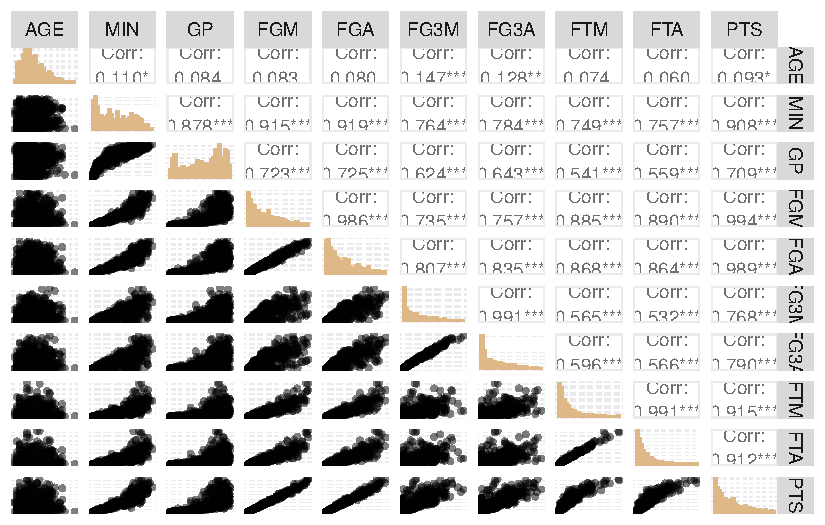
\includegraphics[width=1\textwidth,height=\textheight]{Modelos_files/figure-pdf/unnamed-chunk-4-1.pdf}

En la matriz de dispersión realizada se usó el coeficiente de
correlación de Pearson, el cuál nos muestra que la mayoría de las
variables tienen una alta correlación lineal con la variable respuesta,
puntos realizados en la temporada (PTS).

Se puede evidenciar que entre las variables tambien se presentan algunas
correlaciones casi perfectas, como se presentan entre las variables FGM
y FGA, FG3M y FG3A, y FTM y FTA, lo cual tiene sentido ya que los pares
de variables mencionadas deberían estar relacionadas entre sí, ya que a
nivel general una variable es el número de intentos totales de tiros,
mientras que la otra es cuántos de esos tiros lograron ser encestados.

Por otro lado, se observa una baja correlación lineal entre la variable
AGE y el resto de las variables, incluida la variable respuesta PTS.
Además, en los gráficos de dispersión no se evidencia ningún tipo de
correlación entre estas variables, ya que los datos se encuentran muy
dispersos.

\begin{Shaded}
\begin{Highlighting}[]
\NormalTok{x1 }\OtherTok{\textless{}{-}}\NormalTok{ players }\SpecialCharTok{\%\textgreater{}\%} \FunctionTok{select}\NormalTok{(}\SpecialCharTok{{-}}\FunctionTok{last\_col}\NormalTok{())}
\NormalTok{X }\OtherTok{\textless{}{-}} \FunctionTok{model.matrix}\NormalTok{(}\SpecialCharTok{\textasciitilde{}}\NormalTok{ ., }\AttributeTok{data =}\NormalTok{ x1) }\CommentTok{\# Matriz diseño, con intercepto}
\NormalTok{y }\OtherTok{\textless{}{-}}\NormalTok{ players}\SpecialCharTok{$}\NormalTok{PTS }\CommentTok{\# Variable respuesta}
\end{Highlighting}
\end{Shaded}

\subsubsection{Algoritmo de
Fisher-Scoring}\label{algoritmo-de-fisher-scoring}

\begin{Shaded}
\begin{Highlighting}[]
\CommentTok{\# Creación de la función}

\NormalTok{fisher\_scoring\_poisson }\OtherTok{\textless{}{-}} \ControlFlowTok{function}\NormalTok{(y, X, beta\_init, }\AttributeTok{tol =} \FloatTok{1e{-}7}\NormalTok{, }\AttributeTok{max\_iter =} \DecValTok{100}\NormalTok{)\{}
  \CommentTok{\# Nombramos un objeto donde se guardará el beta inicial (beta\_init)}
\NormalTok{  beta }\OtherTok{\textless{}{-}}\NormalTok{ beta\_init}
  \CommentTok{\# iniciamos el bucle }
  \ControlFlowTok{for}\NormalTok{ (iter }\ControlFlowTok{in} \DecValTok{1}\SpecialCharTok{:}\NormalTok{max\_iter)\{}
    \CommentTok{\# creamos un objeto "eta" que será la parte sistemática del modelo}
\NormalTok{    eta }\OtherTok{\textless{}{-}}\NormalTok{ X }\SpecialCharTok{\%*\%}\NormalTok{ beta}
    \CommentTok{\# creamos un objeto "mu" donde se guarda el despeje de la media de "eta"}
\NormalTok{    mu }\OtherTok{\textless{}{-}} \FunctionTok{exp}\NormalTok{(eta)}
    \CommentTok{\# creamos la matriz diagonal "W"}
\NormalTok{    W }\OtherTok{\textless{}{-}} \FunctionTok{diag}\NormalTok{(}\FunctionTok{as.vector}\NormalTok{(mu))}
    \CommentTok{\# creamos el objeto z (variable de trabajo y\^{}\textasciitilde{})}
\NormalTok{    z }\OtherTok{\textless{}{-}}\NormalTok{ eta }\SpecialCharTok{+}\NormalTok{ (y }\SpecialCharTok{{-}}\NormalTok{ mu) }\SpecialCharTok{/}\NormalTok{ mu}
    \CommentTok{\# obtenemos el nuevo beta}
\NormalTok{    beta\_new }\OtherTok{\textless{}{-}} \FunctionTok{solve}\NormalTok{(}\FunctionTok{t}\NormalTok{(X) }\SpecialCharTok{\%*\%}\NormalTok{ W }\SpecialCharTok{\%*\%}\NormalTok{ X) }\SpecialCharTok{\%*\%}\NormalTok{ (}\FunctionTok{t}\NormalTok{(X) }\SpecialCharTok{\%*\%}\NormalTok{ W }\SpecialCharTok{\%*\%}\NormalTok{ z)}
    
    \CommentTok{\# guardamos la matriz de varianzas y covarianzas de los betas}
    
\NormalTok{    cov\_beta }\OtherTok{\textless{}{-}} \FunctionTok{solve}\NormalTok{(}\FunctionTok{t}\NormalTok{(X) }\SpecialCharTok{\%*\%}\NormalTok{ W }\SpecialCharTok{\%*\%}\NormalTok{ X)}
    
    \ControlFlowTok{if}\NormalTok{ (}\FunctionTok{max}\NormalTok{(}\FunctionTok{abs}\NormalTok{(beta\_new }\SpecialCharTok{{-}}\NormalTok{ beta)) }\SpecialCharTok{\textless{}}\NormalTok{ tol) \{}
      \FunctionTok{message}\NormalTok{(}\StringTok{"El algoritmo convergió en la iteración "}\NormalTok{, iter)}
\NormalTok{      mu\_hat }\OtherTok{\textless{}{-}} \FunctionTok{as.vector}\NormalTok{(}\FunctionTok{exp}\NormalTok{(X }\SpecialCharTok{\%*\%}\NormalTok{ beta\_new))}
      \CommentTok{\# residual crudo}
\NormalTok{      residual }\OtherTok{\textless{}{-}}\NormalTok{ y }\SpecialCharTok{{-}}\NormalTok{ mu\_hat}
      \CommentTok{\# residual de pearson}
\NormalTok{      residual\_pearson }\OtherTok{\textless{}{-}}\NormalTok{ (y }\SpecialCharTok{{-}}\NormalTok{ mu\_hat) }\SpecialCharTok{/} \FunctionTok{sqrt}\NormalTok{(mu\_hat)}
      \CommentTok{\#Residual Anscombe}
\NormalTok{      residual\_anscombe }\OtherTok{\textless{}{-}}\NormalTok{ (}\DecValTok{3}\SpecialCharTok{/}\DecValTok{2}\NormalTok{) }\SpecialCharTok{*}\NormalTok{ (y}\SpecialCharTok{\^{}}\NormalTok{(}\DecValTok{2}\SpecialCharTok{/}\DecValTok{3}\NormalTok{) }\SpecialCharTok{{-}}\NormalTok{ mu\_hat}\SpecialCharTok{\^{}}\NormalTok{(}\DecValTok{2}\SpecialCharTok{/}\DecValTok{3}\NormalTok{)) }\SpecialCharTok{/}\NormalTok{ (mu\_hat}\SpecialCharTok{\^{}}\NormalTok{(}\DecValTok{1}\SpecialCharTok{/}\DecValTok{6}\NormalTok{))}
      \CommentTok{\# Residual de devianza}
\NormalTok{      residual\_deviance }\OtherTok{\textless{}{-}} \FunctionTok{sign}\NormalTok{(y }\SpecialCharTok{{-}}\NormalTok{ mu\_hat) }\SpecialCharTok{*} \FunctionTok{sqrt}\NormalTok{(}\DecValTok{2} \SpecialCharTok{*}\NormalTok{ (y }\SpecialCharTok{*} \FunctionTok{log}\NormalTok{(}\FunctionTok{ifelse}\NormalTok{(y }\SpecialCharTok{==} \DecValTok{0}\NormalTok{, }\DecValTok{1}\NormalTok{, y }\SpecialCharTok{/}\NormalTok{ mu\_hat)) }\SpecialCharTok{{-}}\NormalTok{ (y }\SpecialCharTok{{-}}\NormalTok{ mu\_hat)))}
      \FunctionTok{return}\NormalTok{(}\FunctionTok{list}\NormalTok{( }\AttributeTok{beta =} \FunctionTok{as.vector}\NormalTok{(beta\_new), }\AttributeTok{predichos =}\NormalTok{ mu\_hat, }\AttributeTok{covarianza =}\NormalTok{ cov\_beta, }\AttributeTok{residual =}\NormalTok{ residual,}
                   \AttributeTok{residual\_pearson =}\NormalTok{ residual\_pearson,}
                   \AttributeTok{residual\_anscombe =}\NormalTok{ residual\_anscombe,}
                   \AttributeTok{residual\_deviance =}\NormalTok{ residual\_deviance))}
\NormalTok{    \}}
    
\NormalTok{    beta }\OtherTok{\textless{}{-}}\NormalTok{ beta\_new}
\NormalTok{  \}}
  \FunctionTok{warning}\NormalTok{(}\StringTok{"El algoritmo no convergió"}\NormalTok{)}
  \FunctionTok{return}\NormalTok{(}\ConstantTok{NULL}\NormalTok{)}
\NormalTok{\}}
\end{Highlighting}
\end{Shaded}

\begin{Shaded}
\begin{Highlighting}[]
\CommentTok{\# Ejecutamos la función}

\NormalTok{beta\_inicial }\OtherTok{\textless{}{-}} \FunctionTok{c}\NormalTok{(}\FunctionTok{log}\NormalTok{(}\FunctionTok{mean}\NormalTok{(y)), }\FunctionTok{rep}\NormalTok{(}\DecValTok{0}\NormalTok{, }\FunctionTok{ncol}\NormalTok{(X)}\SpecialCharTok{{-}}\DecValTok{1}\NormalTok{)) }\CommentTok{\# beta inicial}
\NormalTok{regresion\_poisson }\OtherTok{\textless{}{-}} \FunctionTok{fisher\_scoring\_poisson}\NormalTok{(}\AttributeTok{y =}\NormalTok{ y, }\AttributeTok{X =}\NormalTok{ X, }\AttributeTok{beta\_init =}\NormalTok{ beta\_inicial)}
\end{Highlighting}
\end{Shaded}

\begin{verbatim}
El algoritmo convergió en la iteración 7
\end{verbatim}

\begin{Shaded}
\begin{Highlighting}[]
\CommentTok{\# Estimación de los parámetros del modelo}

\FunctionTok{names}\NormalTok{(regresion\_poisson}\SpecialCharTok{$}\NormalTok{beta) }\OtherTok{\textless{}{-}} \FunctionTok{c}\NormalTok{(}\StringTok{"Intercept"}\NormalTok{, }\StringTok{"AGE"}\NormalTok{, }\StringTok{"MIN"}\NormalTok{, }\StringTok{"GP"}\NormalTok{, }\StringTok{"FGM"}\NormalTok{, }\StringTok{"FGA"}\NormalTok{, }\StringTok{"FG3M"}\NormalTok{, }\StringTok{"FG3A"}\NormalTok{, }\StringTok{"FTM"}\NormalTok{, }\StringTok{"FTA"}\NormalTok{)}
\NormalTok{regresion\_poisson}\SpecialCharTok{$}\NormalTok{beta}
\end{Highlighting}
\end{Shaded}

\begin{verbatim}
    Intercept           AGE           MIN            GP           FGM 
 4.1116424116  0.0076175147  0.0000747274  0.0181945865  0.0019076539 
          FGA          FG3M          FG3A           FTM           FTA 
 0.0002784068  0.0036404818 -0.0011454886  0.0001737093  0.0002852445 
\end{verbatim}

Estimación de los parámetros usando la función \texttt{glm} del paquete
\texttt{stats}

\begin{Shaded}
\begin{Highlighting}[]
\NormalTok{modelo\_poisson\_glm }\OtherTok{\textless{}{-}} \FunctionTok{glm}\NormalTok{(y }\SpecialCharTok{\textasciitilde{}}\NormalTok{ X }\SpecialCharTok{{-}} \DecValTok{1}\NormalTok{, }\AttributeTok{family =} \FunctionTok{poisson}\NormalTok{(}\AttributeTok{link =} \StringTok{"log"}\NormalTok{))}

\FunctionTok{names}\NormalTok{(modelo\_poisson\_glm}\SpecialCharTok{$}\NormalTok{coefficients) }\OtherTok{\textless{}{-}} \FunctionTok{names}\NormalTok{(regresion\_poisson}\SpecialCharTok{$}\NormalTok{beta)}
\NormalTok{modelo\_poisson\_glm}\SpecialCharTok{$}\NormalTok{coefficients}
\end{Highlighting}
\end{Shaded}

\begin{verbatim}
    Intercept           AGE           MIN            GP           FGM 
 4.1116424116  0.0076175147  0.0000747274  0.0181945865  0.0019076539 
          FGA          FG3M          FG3A           FTM           FTA 
 0.0002784068  0.0036404818 -0.0011454886  0.0001737093  0.0002852445 
\end{verbatim}

En la siguiente tabla se puede ver la comparación con ambos métodos:

\begin{longtable}[]{@{}
  >{\raggedright\arraybackslash}p{(\columnwidth - 4\tabcolsep) * \real{0.2059}}
  >{\centering\arraybackslash}p{(\columnwidth - 4\tabcolsep) * \real{0.4265}}
  >{\centering\arraybackslash}p{(\columnwidth - 4\tabcolsep) * \real{0.3676}}@{}}
\toprule\noalign{}
\begin{minipage}[b]{\linewidth}\raggedright
Variable
\end{minipage} & \begin{minipage}[b]{\linewidth}\centering
fisher\_scoring\_poisson
\end{minipage} & \begin{minipage}[b]{\linewidth}\centering
glm
\end{minipage} \\
\midrule\noalign{}
\endhead
\bottomrule\noalign{}
\endlastfoot
(Intercept) & \(\hat{\beta_0} = 4.111\) & \(\hat{\beta_0} = 4.112\) \\
AGE & \(\hat{\beta_1} = 0.007617\) & \(\hat{\beta_1} = 0.007618\) \\
MIN & \(\hat{\beta_2} = 0.00007472\) & \(\hat{\beta_2} = 0.00007473\) \\
GP & \(\hat{\beta_3} = 0.01819\) & \(\hat{\beta_3} = 0.01819\) \\
FGM & \(\hat{\beta_4} = 0.001907\) & \(\hat{\beta_4} = 0.001908\) \\
FGA & \(\hat{\beta_5} = 0.0002784\) & \(\hat{\beta_5} = 0.0002784\) \\
FG3M & \(\hat{\beta_6} = 0.003640\) & \(\hat{\beta_6} = 0.003640\) \\
FG3A & \(\hat{\beta_7} = -0.001145\) & \(\hat{\beta_7} = -0.001145\) \\
FTM & \(\hat{\beta_8} = 0.0001737\) & \(\hat{\beta_8} = 0.0001737\) \\
FTA & \(\hat{\beta_9} = 0.0002852\) & \(\hat{\beta_9} = 0.0002852\) \\
\end{longtable}

Los resultados parecen ser exactamente los mismos

\begin{Shaded}
\begin{Highlighting}[]
\FunctionTok{all.equal}\NormalTok{(regresion\_poisson}\SpecialCharTok{$}\NormalTok{beta, modelo\_poisson\_glm}\SpecialCharTok{$}\NormalTok{coefficients)}
\end{Highlighting}
\end{Shaded}

\begin{verbatim}
[1] TRUE
\end{verbatim}

La matriz de covarianza estimada obtenida mediante el algoritmo de
Fisher-Scoring coincide con la obtenida a través de la función
\texttt{glm}, salvo por algunas diferencias numéricas muy pequeñas

\begin{Shaded}
\begin{Highlighting}[]
\FunctionTok{all.equal}\NormalTok{(regresion\_poisson}\SpecialCharTok{$}\NormalTok{covarianza, }\FunctionTok{vcov}\NormalTok{(modelo\_poisson\_glm))}
\end{Highlighting}
\end{Shaded}

\begin{verbatim}
[1] "Attributes: < Component \"dimnames\": Component 1: 1 string mismatch >"
[2] "Attributes: < Component \"dimnames\": Component 2: 1 string mismatch >"
[3] "Mean relative difference: 1.183917e-07"                                
\end{verbatim}

Las desviaciones estándar estimadas con ambos métodos son las
siguientes:

\begin{Shaded}
\begin{Highlighting}[]
\FunctionTok{sqrt}\NormalTok{(}\FunctionTok{diag}\NormalTok{(regresion\_poisson}\SpecialCharTok{$}\NormalTok{covarianza))}
\end{Highlighting}
\end{Shaded}

\begin{verbatim}
 (Intercept)          AGE          MIN           GP          FGM          FGA 
1.573243e-02 4.749512e-04 8.853810e-06 2.315808e-04 7.836140e-05 4.481510e-05 
        FG3M         FG3A          FTM          FTA 
2.317290e-04 1.008010e-04 9.716799e-05 8.408862e-05 
\end{verbatim}

\begin{Shaded}
\begin{Highlighting}[]
\FunctionTok{sqrt}\NormalTok{(}\FunctionTok{diag}\NormalTok{(}\FunctionTok{vcov}\NormalTok{(modelo\_poisson\_glm)))}
\end{Highlighting}
\end{Shaded}

\begin{verbatim}
   Intercept          AGE          MIN           GP          FGM          FGA 
1.573243e-02 4.749512e-04 8.853809e-06 2.315807e-04 7.836140e-05 4.481510e-05 
        FG3M         FG3A          FTM          FTA 
2.317290e-04 1.008010e-04 9.716799e-05 8.408862e-05 
\end{verbatim}

Son exactamente las mismas.

A continuación, se muestran gráficamente los cuatro tipos de residuales
calculados: \emph{residuales crudos}, \emph{residuales de pearson},
\emph{residuales de Anscombe} y \emph{residuales de devianza}

\begin{Shaded}
\begin{Highlighting}[]
\NormalTok{df\_residuals }\OtherTok{\textless{}{-}} \FunctionTok{data.frame}\NormalTok{(}
    \AttributeTok{predichos =}\NormalTok{ regresion\_poisson}\SpecialCharTok{$}\NormalTok{predichos,}
    \AttributeTok{residual =}\NormalTok{ regresion\_poisson}\SpecialCharTok{$}\NormalTok{residual,}
    \AttributeTok{residual\_pearson =}\NormalTok{ regresion\_poisson}\SpecialCharTok{$}\NormalTok{residual\_pearson,}
    \AttributeTok{residual\_anscombe =}\NormalTok{ regresion\_poisson}\SpecialCharTok{$}\NormalTok{residual\_anscombe,}
    \AttributeTok{residual\_deviance =}\NormalTok{ regresion\_poisson}\SpecialCharTok{$}\NormalTok{residual\_deviance}
\NormalTok{  )}
\end{Highlighting}
\end{Shaded}

\begin{Shaded}
\begin{Highlighting}[]
\CommentTok{\# Gráfico de los tres tipos de residuales}

\NormalTok{p1 }\OtherTok{\textless{}{-}} \FunctionTok{ggplot}\NormalTok{(df\_residuals, }\FunctionTok{aes}\NormalTok{(}\AttributeTok{x =}\NormalTok{ predichos, }\AttributeTok{y =}\NormalTok{ residual)) }\SpecialCharTok{+}
    \FunctionTok{geom\_point}\NormalTok{(}\AttributeTok{color =} \StringTok{\textquotesingle{}blue\textquotesingle{}}\NormalTok{) }\SpecialCharTok{+}
    \FunctionTok{labs}\NormalTok{(}\AttributeTok{title =} \StringTok{\textquotesingle{}Residual Crudo\textquotesingle{}}\NormalTok{, }\AttributeTok{x =} \StringTok{\textquotesingle{}Valores Predichos\textquotesingle{}}\NormalTok{, }\AttributeTok{y =} \StringTok{\textquotesingle{}Residual Crudo\textquotesingle{}}\NormalTok{) }\SpecialCharTok{+}
    \FunctionTok{theme\_minimal}\NormalTok{(}\DecValTok{12}\NormalTok{)}

\NormalTok{p2 }\OtherTok{\textless{}{-}} \FunctionTok{ggplot}\NormalTok{(df\_residuals, }\FunctionTok{aes}\NormalTok{(}\AttributeTok{x =}\NormalTok{ predichos, }\AttributeTok{y =}\NormalTok{ residual\_pearson)) }\SpecialCharTok{+}
    \FunctionTok{geom\_point}\NormalTok{(}\AttributeTok{color =} \StringTok{\textquotesingle{}red\textquotesingle{}}\NormalTok{) }\SpecialCharTok{+}
    \FunctionTok{labs}\NormalTok{(}\AttributeTok{title =} \StringTok{\textquotesingle{}Residual de Pearson\textquotesingle{}}\NormalTok{, }\AttributeTok{x =} \StringTok{\textquotesingle{}Valores Predichos\textquotesingle{}}\NormalTok{, }\AttributeTok{y =} \StringTok{\textquotesingle{}Residual de Pearson\textquotesingle{}}\NormalTok{) }\SpecialCharTok{+}
    \FunctionTok{theme\_minimal}\NormalTok{(}\DecValTok{12}\NormalTok{)}

\NormalTok{p3 }\OtherTok{\textless{}{-}} \FunctionTok{ggplot}\NormalTok{(df\_residuals, }\FunctionTok{aes}\NormalTok{(}\AttributeTok{x =}\NormalTok{ predichos, }\AttributeTok{y =}\NormalTok{ residual\_anscombe)) }\SpecialCharTok{+}
    \FunctionTok{geom\_point}\NormalTok{(}\AttributeTok{color =} \StringTok{\textquotesingle{}green\textquotesingle{}}\NormalTok{) }\SpecialCharTok{+}
    \FunctionTok{labs}\NormalTok{(}\AttributeTok{title =} \StringTok{\textquotesingle{}Residual de Anscombe\textquotesingle{}}\NormalTok{, }\AttributeTok{x =} \StringTok{\textquotesingle{}Valores Predichos\textquotesingle{}}\NormalTok{, }\AttributeTok{y =} \StringTok{\textquotesingle{}Residual de Anscombe\textquotesingle{}}\NormalTok{) }\SpecialCharTok{+}
    \FunctionTok{theme\_minimal}\NormalTok{(}\DecValTok{12}\NormalTok{)}

\NormalTok{p4 }\OtherTok{\textless{}{-}} \FunctionTok{ggplot}\NormalTok{(df\_residuals, }\FunctionTok{aes}\NormalTok{(}\AttributeTok{x =}\NormalTok{ predichos, }\AttributeTok{y =}\NormalTok{ residual\_deviance)) }\SpecialCharTok{+}
    \FunctionTok{geom\_point}\NormalTok{(}\AttributeTok{color =} \StringTok{\textquotesingle{}orange\textquotesingle{}}\NormalTok{) }\SpecialCharTok{+}
    \FunctionTok{labs}\NormalTok{(}\AttributeTok{title =} \StringTok{\textquotesingle{}Residual de Devianza\textquotesingle{}}\NormalTok{, }\AttributeTok{x =} \StringTok{\textquotesingle{}Valores Predichos\textquotesingle{}}\NormalTok{, }\AttributeTok{y =} \StringTok{\textquotesingle{}Residual de Devianza\textquotesingle{}}\NormalTok{) }\SpecialCharTok{+}
    \FunctionTok{theme\_minimal}\NormalTok{(}\DecValTok{12}\NormalTok{)}
\end{Highlighting}
\end{Shaded}

\begin{Shaded}
\begin{Highlighting}[]
\NormalTok{p1; p2; p3; p4}
\end{Highlighting}
\end{Shaded}

\begin{figure}

\begin{minipage}{0.50\linewidth}
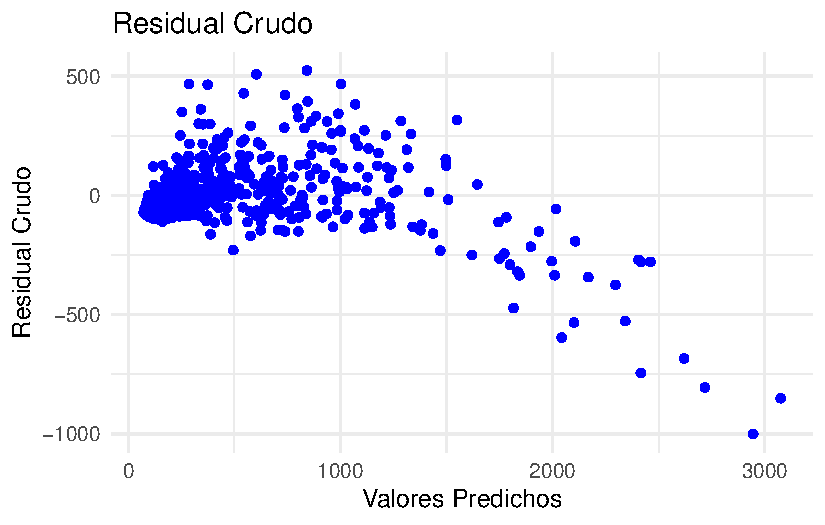
\includegraphics{Modelos_files/figure-pdf/unnamed-chunk-14-1.pdf}\end{minipage}%
%
\begin{minipage}{0.50\linewidth}
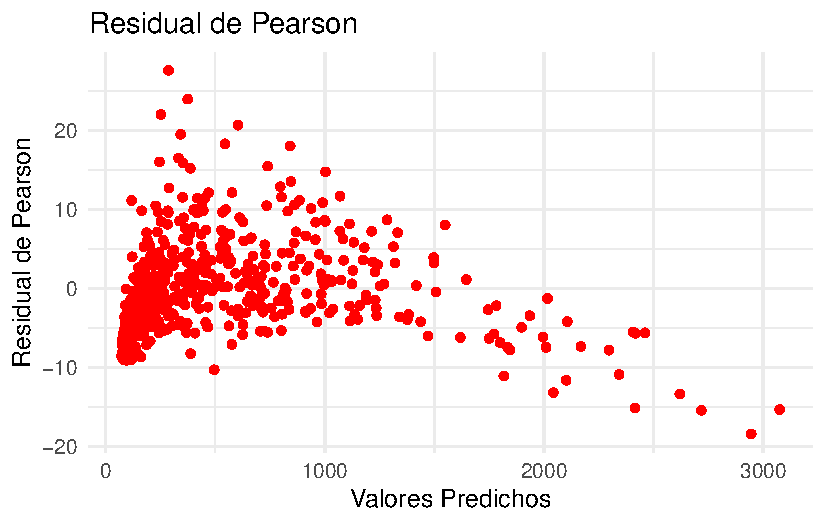
\includegraphics{Modelos_files/figure-pdf/unnamed-chunk-14-2.pdf}\end{minipage}%
\newline
\begin{minipage}{0.50\linewidth}
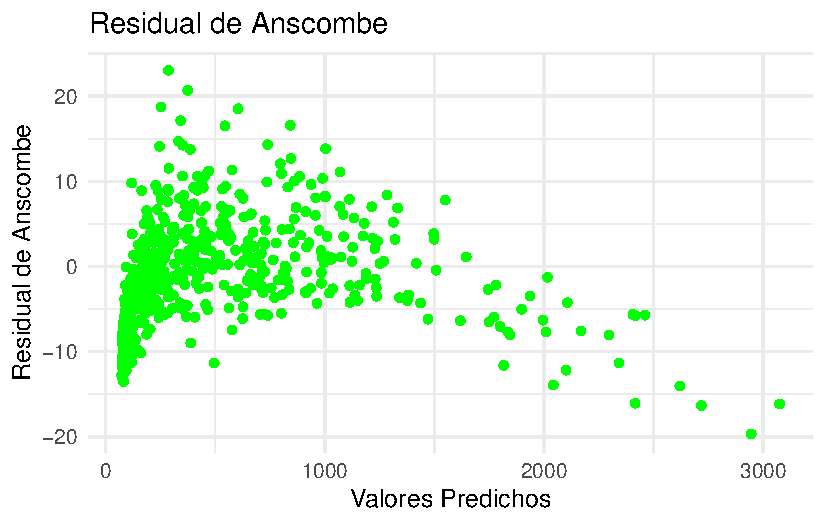
\includegraphics{Modelos_files/figure-pdf/unnamed-chunk-14-3.pdf}\end{minipage}%
%
\begin{minipage}{0.50\linewidth}
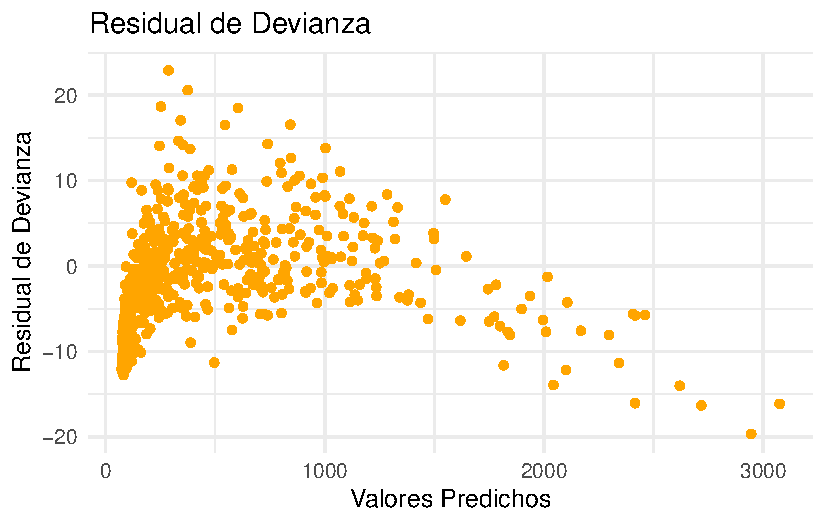
\includegraphics{Modelos_files/figure-pdf/unnamed-chunk-14-4.pdf}\end{minipage}%

\end{figure}%

\subsection{Ejemplo 2 para distribución
Poisson}\label{ejemplo-2-para-distribuciuxf3n-poisson}

\begin{Shaded}
\begin{Highlighting}[]
\NormalTok{crabs }\OtherTok{\textless{}{-}} \FunctionTok{data.frame}\NormalTok{(}
  \AttributeTok{C =} \FunctionTok{as.factor}\NormalTok{(}\FunctionTok{c}\NormalTok{(}\DecValTok{2}\NormalTok{,}\DecValTok{3}\NormalTok{,}\DecValTok{3}\NormalTok{,}\DecValTok{2}\NormalTok{,}\DecValTok{2}\NormalTok{,}\DecValTok{1}\NormalTok{,}\DecValTok{2}\NormalTok{,}\DecValTok{1}\NormalTok{,}\DecValTok{3}\NormalTok{,}\DecValTok{2}\NormalTok{,}\DecValTok{2}\NormalTok{,}\DecValTok{2}\NormalTok{,}\DecValTok{1}\NormalTok{,}\DecValTok{2}\NormalTok{,}\DecValTok{2}\NormalTok{,}\DecValTok{2}\NormalTok{,}\DecValTok{2}\NormalTok{,}\DecValTok{3}\NormalTok{,}\DecValTok{3}\NormalTok{,}\DecValTok{2}\NormalTok{,}\DecValTok{2}\NormalTok{,}\DecValTok{2}\NormalTok{,}\DecValTok{2}\NormalTok{,}\DecValTok{3}\NormalTok{,}\DecValTok{3}\NormalTok{,}\DecValTok{2}\NormalTok{,}\DecValTok{2}\NormalTok{,}\DecValTok{2}\NormalTok{,}\DecValTok{2}\NormalTok{,}\DecValTok{3}\NormalTok{,}\DecValTok{3}\NormalTok{,}\DecValTok{3}\NormalTok{,}\DecValTok{2}\NormalTok{,}\DecValTok{3}\NormalTok{,}\DecValTok{2}\NormalTok{,}\DecValTok{2}\NormalTok{,}
        \DecValTok{2}\NormalTok{,}\DecValTok{3}\NormalTok{,}\DecValTok{3}\NormalTok{,}\DecValTok{2}\NormalTok{,}\DecValTok{2}\NormalTok{,}\DecValTok{1}\NormalTok{,}\DecValTok{1}\NormalTok{,}\DecValTok{3}\NormalTok{,}\DecValTok{3}\NormalTok{,}\DecValTok{3}\NormalTok{,}\DecValTok{2}\NormalTok{,}\DecValTok{2}\NormalTok{,}\DecValTok{3}\NormalTok{,}\DecValTok{3}\NormalTok{,}\DecValTok{3}\NormalTok{,}\DecValTok{3}\NormalTok{,}\DecValTok{2}\NormalTok{,}\DecValTok{2}\NormalTok{,}\DecValTok{3}\NormalTok{,}\DecValTok{2}\NormalTok{,}\DecValTok{3}\NormalTok{,}\DecValTok{2}\NormalTok{,}\DecValTok{1}\NormalTok{,}\DecValTok{3}\NormalTok{,}\DecValTok{2}\NormalTok{,}\DecValTok{3}\NormalTok{,}\DecValTok{1}\NormalTok{,}\DecValTok{1}\NormalTok{,}\DecValTok{2}\NormalTok{,}\DecValTok{2}\NormalTok{,}\DecValTok{3}\NormalTok{,}\DecValTok{2}\NormalTok{,}\DecValTok{3}\NormalTok{,}\DecValTok{2}\NormalTok{,}\DecValTok{3}\NormalTok{,}\DecValTok{2}\NormalTok{,}
        \DecValTok{2}\NormalTok{,}\DecValTok{2}\NormalTok{,}\DecValTok{3}\NormalTok{,}\DecValTok{3}\NormalTok{,}\DecValTok{2}\NormalTok{,}\DecValTok{2}\NormalTok{,}\DecValTok{1}\NormalTok{,}\DecValTok{2}\NormalTok{,}\DecValTok{2}\NormalTok{,}\DecValTok{2}\NormalTok{,}\DecValTok{1}\NormalTok{,}\DecValTok{2}\NormalTok{,}\DecValTok{2}\NormalTok{,}\DecValTok{3}\NormalTok{,}\DecValTok{2}\NormalTok{,}\DecValTok{2}\NormalTok{,}\DecValTok{1}\NormalTok{,}\DecValTok{2}\NormalTok{,}\DecValTok{3}\NormalTok{,}\DecValTok{3}\NormalTok{,}\DecValTok{3}\NormalTok{,}\DecValTok{3}\NormalTok{,}\DecValTok{3}\NormalTok{,}\DecValTok{1}\NormalTok{,}\DecValTok{3}\NormalTok{,}\DecValTok{2}\NormalTok{,}\DecValTok{3}\NormalTok{,}\DecValTok{2}\NormalTok{)),}
  \AttributeTok{S =} \FunctionTok{as.factor}\NormalTok{(}\FunctionTok{c}\NormalTok{(}\DecValTok{3}\NormalTok{,}\DecValTok{3}\NormalTok{,}\DecValTok{3}\NormalTok{,}\DecValTok{3}\NormalTok{,}\DecValTok{1}\NormalTok{,}\DecValTok{2}\NormalTok{,}\DecValTok{1}\NormalTok{,}\DecValTok{1}\NormalTok{,}\DecValTok{2}\NormalTok{,}\DecValTok{2}\NormalTok{,}\DecValTok{1}\NormalTok{,}\DecValTok{3}\NormalTok{,}\DecValTok{1}\NormalTok{,}\DecValTok{1}\NormalTok{,}\DecValTok{1}\NormalTok{,}\DecValTok{2}\NormalTok{,}\DecValTok{2}\NormalTok{,}\DecValTok{2}\NormalTok{,}\DecValTok{2}\NormalTok{,}\DecValTok{2}\NormalTok{,}\DecValTok{2}\NormalTok{,}\DecValTok{1}\NormalTok{,}\DecValTok{2}\NormalTok{,}\DecValTok{3}\NormalTok{,}\DecValTok{3}\NormalTok{,}\DecValTok{1}\NormalTok{,}\DecValTok{3}\NormalTok{,}\DecValTok{1}\NormalTok{,}\DecValTok{1}\NormalTok{,}\DecValTok{3}\NormalTok{,}\DecValTok{3}\NormalTok{,}\DecValTok{3}\NormalTok{,}\DecValTok{3}\NormalTok{,}\DecValTok{2}\NormalTok{,}\DecValTok{2}\NormalTok{,}\DecValTok{1}\NormalTok{,}
        \DecValTok{1}\NormalTok{,}\DecValTok{3}\NormalTok{,}\DecValTok{2}\NormalTok{,}\DecValTok{1}\NormalTok{,}\DecValTok{3}\NormalTok{,}\DecValTok{3}\NormalTok{,}\DecValTok{1}\NormalTok{,}\DecValTok{2}\NormalTok{,}\DecValTok{3}\NormalTok{,}\DecValTok{2}\NormalTok{,}\DecValTok{1}\NormalTok{,}\DecValTok{1}\NormalTok{,}\DecValTok{3}\NormalTok{,}\DecValTok{1}\NormalTok{,}\DecValTok{2}\NormalTok{,}\DecValTok{3}\NormalTok{,}\DecValTok{2}\NormalTok{,}\DecValTok{2}\NormalTok{,}\DecValTok{1}\NormalTok{,}\DecValTok{2}\NormalTok{,}\DecValTok{1}\NormalTok{,}\DecValTok{1}\NormalTok{,}\DecValTok{3}\NormalTok{,}\DecValTok{1}\NormalTok{,}\DecValTok{3}\NormalTok{,}\DecValTok{3}\NormalTok{,}\DecValTok{1}\NormalTok{,}\DecValTok{1}\NormalTok{,}\DecValTok{2}\NormalTok{,}\DecValTok{1}\NormalTok{,}\DecValTok{2}\NormalTok{,}\DecValTok{2}\NormalTok{,}\DecValTok{2}\NormalTok{,}\DecValTok{2}\NormalTok{,}\DecValTok{1}\NormalTok{,}\DecValTok{3}\NormalTok{,}
        \DecValTok{3}\NormalTok{,}\DecValTok{3}\NormalTok{,}\DecValTok{3}\NormalTok{,}\DecValTok{2}\NormalTok{,}\DecValTok{2}\NormalTok{,}\DecValTok{1}\NormalTok{,}\DecValTok{1}\NormalTok{,}\DecValTok{2}\NormalTok{,}\DecValTok{2}\NormalTok{,}\DecValTok{2}\NormalTok{,}\DecValTok{2}\NormalTok{,}\DecValTok{3}\NormalTok{,}\DecValTok{3}\NormalTok{,}\DecValTok{3}\NormalTok{,}\DecValTok{3}\NormalTok{,}\DecValTok{3}\NormalTok{,}\DecValTok{3}\NormalTok{,}\DecValTok{3}\NormalTok{,}\DecValTok{3}\NormalTok{,}\DecValTok{2}\NormalTok{,}\DecValTok{3}\NormalTok{,}\DecValTok{3}\NormalTok{,}\DecValTok{3}\NormalTok{,}\DecValTok{3}\NormalTok{,}\DecValTok{3}\NormalTok{,}\DecValTok{3}\NormalTok{,}\DecValTok{2}\NormalTok{,}\DecValTok{1}\NormalTok{)),}
  \AttributeTok{W =} \FunctionTok{c}\NormalTok{(}\FloatTok{28.3}\NormalTok{,}\FloatTok{26.0}\NormalTok{,}\FloatTok{26.0}\NormalTok{,}\FloatTok{21.0}\NormalTok{,}\FloatTok{21.0}\NormalTok{,}\FloatTok{25.0}\NormalTok{,}\FloatTok{26.0}\NormalTok{,}\FloatTok{24.9}\NormalTok{,}\FloatTok{25.0}\NormalTok{,}\FloatTok{24.7}\NormalTok{,}\FloatTok{26.5}\NormalTok{,}\FloatTok{24.8}\NormalTok{,}\FloatTok{24.9}\NormalTok{,}\FloatTok{26.0}\NormalTok{,}
        \FloatTok{28.7}\NormalTok{,}\FloatTok{30.3}\NormalTok{,}\FloatTok{26.2}\NormalTok{,}\FloatTok{27.5}\NormalTok{,}\FloatTok{30.0}\NormalTok{,}\FloatTok{28.2}\NormalTok{,}\FloatTok{30.5}\NormalTok{,}\FloatTok{30.3}\NormalTok{,}\FloatTok{30.0}\NormalTok{,}\FloatTok{26.2}\NormalTok{,}\FloatTok{28.5}\NormalTok{,}\FloatTok{29.5}\NormalTok{,}\FloatTok{27.0}\NormalTok{,}\FloatTok{29.0}\NormalTok{,}
        \FloatTok{28.7}\NormalTok{,}\FloatTok{26.5}\NormalTok{,}\FloatTok{26.5}\NormalTok{,}\FloatTok{27.3}\NormalTok{,}\FloatTok{26.3}\NormalTok{,}\FloatTok{30.0}\NormalTok{,}\FloatTok{29.0}\NormalTok{,}\FloatTok{27.2}\NormalTok{,}\FloatTok{27.0}\NormalTok{,}\FloatTok{26.5}\NormalTok{,}\FloatTok{26.5}\NormalTok{,}\FloatTok{25.5}\NormalTok{,}\FloatTok{26.5}\NormalTok{,}\FloatTok{26.5}\NormalTok{,}
        \FloatTok{22.0}\NormalTok{,}\FloatTok{27.3}\NormalTok{,}\FloatTok{26.6}\NormalTok{,}\FloatTok{25.0}\NormalTok{,}\FloatTok{25.0}\NormalTok{,}\FloatTok{30.2}\NormalTok{,}\FloatTok{28.7}\NormalTok{,}\FloatTok{24.9}\NormalTok{,}\FloatTok{24.5}\NormalTok{,}\FloatTok{25.2}\NormalTok{,}\FloatTok{24.0}\NormalTok{,}\FloatTok{22.9}\NormalTok{,}\FloatTok{26.2}\NormalTok{,}\FloatTok{24.4}\NormalTok{,}
        \FloatTok{26.3}\NormalTok{,}\FloatTok{24.5}\NormalTok{,}\FloatTok{27.9}\NormalTok{,}\FloatTok{30.5}\NormalTok{,}\FloatTok{28.2}\NormalTok{,}\FloatTok{27.6}\NormalTok{,}\FloatTok{23.0}\NormalTok{,}\FloatTok{23.9}\NormalTok{,}\FloatTok{22.9}\NormalTok{,}\FloatTok{25.8}\NormalTok{,}\FloatTok{25.8}\NormalTok{,}\FloatTok{24.1}\NormalTok{,}\FloatTok{28.0}\NormalTok{,}\FloatTok{26.0}\NormalTok{,}
        \FloatTok{24.5}\NormalTok{,}\FloatTok{24.5}\NormalTok{,}\FloatTok{24.2}\NormalTok{,}\FloatTok{28.5}\NormalTok{,}\FloatTok{24.7}\NormalTok{,}\FloatTok{29.0}\NormalTok{,}\FloatTok{27.0}\NormalTok{,}\FloatTok{23.7}\NormalTok{,}\FloatTok{27.0}\NormalTok{,}\FloatTok{24.2}\NormalTok{,}\FloatTok{24.2}\NormalTok{,}\FloatTok{25.1}\NormalTok{,}\FloatTok{27.5}\NormalTok{,}\FloatTok{29.3}\NormalTok{,}
        \FloatTok{26.3}\NormalTok{,}\FloatTok{29.4}\NormalTok{,}\FloatTok{26.2}\NormalTok{,}\FloatTok{26.2}\NormalTok{,}\FloatTok{24.1}\NormalTok{,}\FloatTok{27.0}\NormalTok{,}\FloatTok{26.5}\NormalTok{,}\FloatTok{28.5}\NormalTok{,}\FloatTok{24.7}\NormalTok{,}\FloatTok{25.2}\NormalTok{,}\FloatTok{25.3}\NormalTok{,}\FloatTok{25.3}\NormalTok{,}\FloatTok{29.3}\NormalTok{,}\FloatTok{27.4}\NormalTok{,}
        \FloatTok{28.0}\NormalTok{,}\FloatTok{24.5}\NormalTok{),}
  \AttributeTok{Wt =} \FunctionTok{c}\NormalTok{(}\FloatTok{3.05}\NormalTok{,}\FloatTok{2.60}\NormalTok{,}\FloatTok{2.45}\NormalTok{,}\FloatTok{1.85}\NormalTok{,}\FloatTok{2.05}\NormalTok{,}\FloatTok{2.30}\NormalTok{,}\FloatTok{2.10}\NormalTok{,}\FloatTok{2.10}\NormalTok{,}\FloatTok{2.00}\NormalTok{,}\FloatTok{1.90}\NormalTok{,}\FloatTok{2.80}\NormalTok{,}\FloatTok{2.10}\NormalTok{,}\FloatTok{2.10}\NormalTok{,}\FloatTok{2.50}\NormalTok{,}
         \FloatTok{3.20}\NormalTok{,}\FloatTok{3.60}\NormalTok{,}\FloatTok{2.20}\NormalTok{,}\FloatTok{2.75}\NormalTok{,}\FloatTok{3.05}\NormalTok{,}\FloatTok{2.95}\NormalTok{,}\FloatTok{3.50}\NormalTok{,}\FloatTok{3.00}\NormalTok{,}\FloatTok{3.40}\NormalTok{,}\FloatTok{2.30}\NormalTok{,}\FloatTok{2.40}\NormalTok{,}\FloatTok{2.55}\NormalTok{,}\FloatTok{2.25}\NormalTok{,}\FloatTok{2.30}\NormalTok{,}
         \FloatTok{3.20}\NormalTok{,}\FloatTok{1.30}\NormalTok{,}\FloatTok{1.97}\NormalTok{,}\FloatTok{2.90}\NormalTok{,}\FloatTok{2.30}\NormalTok{,}\FloatTok{3.05}\NormalTok{,}\FloatTok{3.30}\NormalTok{,}\FloatTok{2.75}\NormalTok{,}\FloatTok{2.25}\NormalTok{,}\FloatTok{2.00}\NormalTok{,}\FloatTok{2.20}\NormalTok{,}\FloatTok{2.25}\NormalTok{,}\FloatTok{1.97}\NormalTok{,}\FloatTok{1.60}\NormalTok{,}
         \FloatTok{1.90}\NormalTok{,}\FloatTok{2.90}\NormalTok{,}\FloatTok{2.30}\NormalTok{,}\FloatTok{2.10}\NormalTok{,}\FloatTok{2.10}\NormalTok{,}\FloatTok{3.28}\NormalTok{,}\FloatTok{3.20}\NormalTok{,}\FloatTok{2.30}\NormalTok{,}\FloatTok{2.05}\NormalTok{,}\FloatTok{2.10}\NormalTok{,}\FloatTok{2.00}\NormalTok{,}\FloatTok{1.60}\NormalTok{,}\FloatTok{2.40}\NormalTok{,}\FloatTok{1.90}\NormalTok{,}
         \FloatTok{2.05}\NormalTok{,}\FloatTok{1.95}\NormalTok{,}\FloatTok{3.05}\NormalTok{,}\FloatTok{3.20}\NormalTok{,}\FloatTok{2.80}\NormalTok{,}\FloatTok{2.85}\NormalTok{,}\FloatTok{3.00}\NormalTok{,}\FloatTok{1.85}\NormalTok{,}\FloatTok{1.90}\NormalTok{,}\FloatTok{2.20}\NormalTok{,}\FloatTok{2.20}\NormalTok{,}\FloatTok{1.80}\NormalTok{,}\FloatTok{2.62}\NormalTok{,}\FloatTok{2.30}\NormalTok{,}
         \FloatTok{2.00}\NormalTok{,}\FloatTok{2.00}\NormalTok{,}\FloatTok{2.20}\NormalTok{,}\FloatTok{3.00}\NormalTok{,}\FloatTok{2.55}\NormalTok{,}\FloatTok{3.10}\NormalTok{,}\FloatTok{2.95}\NormalTok{,}\FloatTok{1.80}\NormalTok{,}\FloatTok{2.00}\NormalTok{,}\FloatTok{2.20}\NormalTok{,}\FloatTok{1.65}\NormalTok{,}\FloatTok{1.80}\NormalTok{,}\FloatTok{2.30}\NormalTok{,}\FloatTok{3.23}\NormalTok{,}
         \FloatTok{2.90}\NormalTok{,}\FloatTok{3.10}\NormalTok{,}\FloatTok{2.30}\NormalTok{,}\FloatTok{2.17}\NormalTok{,}\FloatTok{1.95}\NormalTok{,}\FloatTok{2.63}\NormalTok{,}\FloatTok{2.35}\NormalTok{,}\FloatTok{3.00}\NormalTok{,}\FloatTok{2.55}\NormalTok{,}\FloatTok{2.00}\NormalTok{,}\FloatTok{1.90}\NormalTok{,}\FloatTok{1.90}\NormalTok{,}\FloatTok{3.23}\NormalTok{,}\FloatTok{2.90}\NormalTok{,}
         \FloatTok{3.00}\NormalTok{,}\FloatTok{2.00}\NormalTok{),}
  \AttributeTok{Sa =} \FunctionTok{c}\NormalTok{(}\DecValTok{8}\NormalTok{,}\DecValTok{4}\NormalTok{,}\DecValTok{3}\NormalTok{,}\DecValTok{0}\NormalTok{,}\DecValTok{0}\NormalTok{,}\DecValTok{3}\NormalTok{,}\DecValTok{0}\NormalTok{,}\DecValTok{1}\NormalTok{,}\DecValTok{3}\NormalTok{,}\DecValTok{0}\NormalTok{,}\DecValTok{4}\NormalTok{,}\DecValTok{0}\NormalTok{,}\DecValTok{1}\NormalTok{,}\DecValTok{1}\NormalTok{,}\DecValTok{0}\NormalTok{,}\DecValTok{4}\NormalTok{,}\DecValTok{3}\NormalTok{,}\DecValTok{0}\NormalTok{,}\DecValTok{5}\NormalTok{,}\DecValTok{4}\NormalTok{,}\DecValTok{6}\NormalTok{,}\DecValTok{4}\NormalTok{,}\DecValTok{4}\NormalTok{,}\DecValTok{0}\NormalTok{,}\DecValTok{3}\NormalTok{,}\DecValTok{0}\NormalTok{,}\DecValTok{3}\NormalTok{,}\DecValTok{0}\NormalTok{,}\DecValTok{0}\NormalTok{,}\DecValTok{0}\NormalTok{,}\DecValTok{1}\NormalTok{,}\DecValTok{1}\NormalTok{,}\DecValTok{2}\NormalTok{,}\DecValTok{4}\NormalTok{,}\DecValTok{0}\NormalTok{,}
         \DecValTok{4}\NormalTok{,}\DecValTok{4}\NormalTok{,}\DecValTok{0}\NormalTok{,}\DecValTok{0}\NormalTok{,}\DecValTok{0}\NormalTok{,}\DecValTok{0}\NormalTok{,}\DecValTok{0}\NormalTok{,}\DecValTok{0}\NormalTok{,}\DecValTok{1}\NormalTok{,}\DecValTok{1}\NormalTok{,}\DecValTok{2}\NormalTok{,}\DecValTok{0}\NormalTok{,}\DecValTok{2}\NormalTok{,}\DecValTok{1}\NormalTok{,}\DecValTok{0}\NormalTok{,}\DecValTok{0}\NormalTok{,}\DecValTok{1}\NormalTok{,}\DecValTok{0}\NormalTok{,}\DecValTok{0}\NormalTok{,}\DecValTok{0}\NormalTok{,}\DecValTok{0}\NormalTok{,}\DecValTok{0}\NormalTok{,}\DecValTok{1}\NormalTok{,}\DecValTok{0}\NormalTok{,}\DecValTok{3}\NormalTok{,}\DecValTok{3}\NormalTok{,}\DecValTok{2}\NormalTok{,}\DecValTok{3}\NormalTok{,}\DecValTok{0}\NormalTok{,}\DecValTok{0}\NormalTok{,}\DecValTok{0}\NormalTok{,}\DecValTok{2}\NormalTok{,}\DecValTok{1}\NormalTok{,}\DecValTok{0}\NormalTok{,}\DecValTok{1}\NormalTok{,}
         \DecValTok{0}\NormalTok{,}\DecValTok{0}\NormalTok{,}\DecValTok{0}\NormalTok{,}\DecValTok{1}\NormalTok{,}\DecValTok{0}\NormalTok{,}\DecValTok{4}\NormalTok{,}\DecValTok{1}\NormalTok{,}\DecValTok{0}\NormalTok{,}\DecValTok{3}\NormalTok{,}\DecValTok{3}\NormalTok{,}\DecValTok{3}\NormalTok{,}\DecValTok{0}\NormalTok{,}\DecValTok{6}\NormalTok{,}\DecValTok{12}\NormalTok{,}\DecValTok{0}\NormalTok{,}\DecValTok{3}\NormalTok{,}\DecValTok{0}\NormalTok{,}\DecValTok{2}\NormalTok{,}\DecValTok{1}\NormalTok{,}\DecValTok{4}\NormalTok{,}\DecValTok{0}\NormalTok{,}\DecValTok{1}\NormalTok{,}\DecValTok{0}\NormalTok{,}\DecValTok{1}\NormalTok{,}\DecValTok{2}\NormalTok{,}\DecValTok{2}\NormalTok{,}\DecValTok{5}\NormalTok{,}\DecValTok{4}\NormalTok{,}\DecValTok{2}\NormalTok{,}\DecValTok{0}\NormalTok{)}
\NormalTok{)}
\end{Highlighting}
\end{Shaded}

Usando los datos obtenidos del libro ``An Introduction to Categorycal
Data Analysis Alan Agresti segunda edición, donde se registraron datos
del número de satélites (Sa) que tiene una cangreja de acuerdo al color
(C), condición de la espina (S), ancho (W) y peso (Wt):

\begin{longtable}[]{@{}lc@{}}
\toprule\noalign{}
Variable & Tipo de Variables \\
\midrule\noalign{}
\endhead
\bottomrule\noalign{}
\endlastfoot
C & Cualitativa nominal \\
S & Cualitativa nominal \\
W & Cuantitativa continua \\
Wt & Cuantitativa continua \\
Sa & Cuantitativa discreta \\
\end{longtable}

\begin{Shaded}
\begin{Highlighting}[]
\NormalTok{crabs[,}\SpecialCharTok{{-}}\FunctionTok{c}\NormalTok{(}\DecValTok{1}\NormalTok{,}\DecValTok{2}\NormalTok{)] }\SpecialCharTok{\%\textgreater{}\%}
  \FunctionTok{ggpairs}\NormalTok{(}
    \AttributeTok{upper =} \FunctionTok{list}\NormalTok{(}\AttributeTok{continuous =} \FunctionTok{wrap}\NormalTok{(}\StringTok{"cor"}\NormalTok{, }\AttributeTok{size =} \DecValTok{3}\NormalTok{)),}
    \AttributeTok{diag =} \FunctionTok{list}\NormalTok{(}\AttributeTok{continuous =} \FunctionTok{wrap}\NormalTok{(}\StringTok{"barDiag"}\NormalTok{, }\AttributeTok{colour =} \StringTok{"burlywood"}\NormalTok{)),}
    \AttributeTok{lower =} \FunctionTok{list}\NormalTok{(}\AttributeTok{continuous =} \FunctionTok{wrap}\NormalTok{(}\StringTok{"points"}\NormalTok{, }\AttributeTok{alpha =} \FloatTok{0.5}\NormalTok{, }\AttributeTok{shape =} \DecValTok{20}\NormalTok{, }
                                   \AttributeTok{fill =} \StringTok{"lightblue"}\NormalTok{)),}
    \AttributeTok{axisLabels =} \StringTok{"none"}\NormalTok{)}
\end{Highlighting}
\end{Shaded}

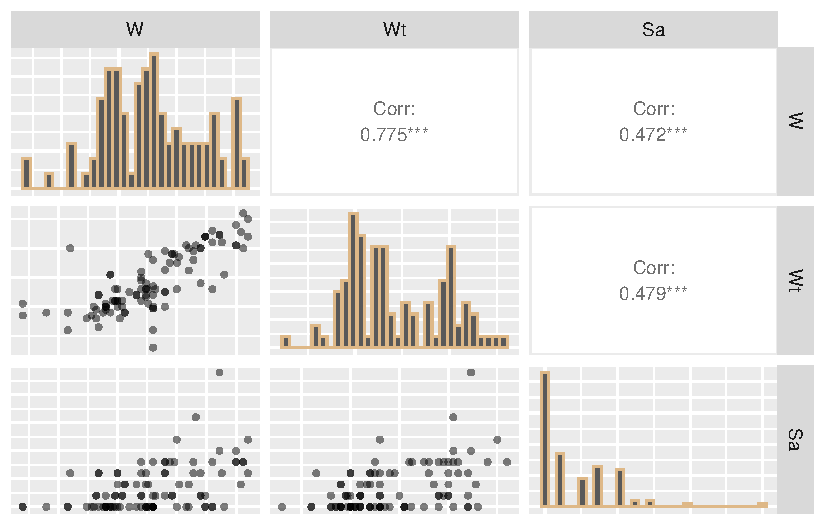
\includegraphics[width=1\textwidth,height=\textheight]{Modelos_files/figure-pdf/unnamed-chunk-16-1.pdf}

\begin{Shaded}
\begin{Highlighting}[]
\NormalTok{X.c }\OtherTok{\textless{}{-}} \FunctionTok{model.matrix}\NormalTok{(}\SpecialCharTok{\textasciitilde{}}\NormalTok{.,}\AttributeTok{data=}\NormalTok{crabs[,}\SpecialCharTok{{-}}\DecValTok{5}\NormalTok{])}
\NormalTok{modelos\_crangrejos }\OtherTok{\textless{}{-}} \FunctionTok{fisher\_scoring\_poisson}\NormalTok{(crabs[,}\DecValTok{5}\NormalTok{],}\AttributeTok{X =}\NormalTok{ X.c,}\AttributeTok{beta\_init =} \FunctionTok{c}\NormalTok{(}\FunctionTok{log}\NormalTok{(}\FunctionTok{mean}\NormalTok{(crabs[,}\DecValTok{5}\NormalTok{])),}\FunctionTok{rep}\NormalTok{(}\DecValTok{0}\NormalTok{, }\FunctionTok{ncol}\NormalTok{(X.c)}\SpecialCharTok{{-}}\DecValTok{1}\NormalTok{)))}
\end{Highlighting}
\end{Shaded}

\begin{verbatim}
El algoritmo convergió en la iteración 6
\end{verbatim}

\begin{Shaded}
\begin{Highlighting}[]
\FunctionTok{names}\NormalTok{(modelos\_crangrejos}\SpecialCharTok{$}\NormalTok{beta) }\OtherTok{\textless{}{-}} \FunctionTok{c}\NormalTok{(}\StringTok{"Intercept"}\NormalTok{, }\StringTok{"C2"}\NormalTok{, }\StringTok{"C3"}\NormalTok{ , }\StringTok{"S2"}\NormalTok{, }\StringTok{"S3"}\NormalTok{ , }\StringTok{"W"}\NormalTok{, }\StringTok{"Wt"}\NormalTok{)}
\NormalTok{modelos\_crangrejos}\SpecialCharTok{$}\NormalTok{beta}
\end{Highlighting}
\end{Shaded}

\begin{verbatim}
 Intercept         C2         C3         S2         S3          W         Wt 
-6.4407728 -0.4973794 -0.8020200  0.5369707  0.6290147  0.2159377  0.4628472 
\end{verbatim}

\begin{Shaded}
\begin{Highlighting}[]
\NormalTok{modelo\_cangrejos\_glm }\OtherTok{\textless{}{-}} \FunctionTok{glm}\NormalTok{(crabs[,}\DecValTok{5}\NormalTok{] }\SpecialCharTok{\textasciitilde{}}\NormalTok{ X.c }\SpecialCharTok{{-}} \DecValTok{1}\NormalTok{, }\AttributeTok{family =} \FunctionTok{poisson}\NormalTok{(}\AttributeTok{link =} \StringTok{"log"}\NormalTok{))}

\FunctionTok{names}\NormalTok{(modelo\_cangrejos\_glm}\SpecialCharTok{$}\NormalTok{coefficients) }\OtherTok{\textless{}{-}} \FunctionTok{names}\NormalTok{(modelos\_crangrejos}\SpecialCharTok{$}\NormalTok{beta)}
\NormalTok{modelo\_cangrejos\_glm}\SpecialCharTok{$}\NormalTok{coefficients}
\end{Highlighting}
\end{Shaded}

\begin{verbatim}
 Intercept         C2         C3         S2         S3          W         Wt 
-6.4407727 -0.4973794 -0.8020200  0.5369707  0.6290147  0.2159377  0.4628472 
\end{verbatim}

En la siguiente tabla se puede ver la comparación con ambos métodos:

\begin{longtable}[]{@{}
  >{\raggedright\arraybackslash}p{(\columnwidth - 4\tabcolsep) * \real{0.2059}}
  >{\centering\arraybackslash}p{(\columnwidth - 4\tabcolsep) * \real{0.4265}}
  >{\centering\arraybackslash}p{(\columnwidth - 4\tabcolsep) * \real{0.3676}}@{}}
\toprule\noalign{}
\begin{minipage}[b]{\linewidth}\raggedright
Variable
\end{minipage} & \begin{minipage}[b]{\linewidth}\centering
fisher\_scoring\_poisson
\end{minipage} & \begin{minipage}[b]{\linewidth}\centering
glm
\end{minipage} \\
\midrule\noalign{}
\endhead
\bottomrule\noalign{}
\endlastfoot
(Intercept) & \(\hat{\beta}_0 = -6.4407728\) &
\(\hat{\beta}_0 = -6.4407727\) \\
C2 & \(\hat{\beta}_1 = -0.4973794\) & \(\hat{\beta}_1 = -0.4973794\) \\
C3 & \(\hat{\beta}_2 = -0.8020200\) & \(\hat{\beta}_2 = -0.8020200\) \\
S2 & \(\hat{\beta}_3 = 0.5369707\) & \(\hat{\beta}_3 = 0.5369707\) \\
S3 & \(\hat{\beta}_4 = 0.6290147\) & \(\hat{\beta}_4 = 0.6290147\) \\
W & \(\hat{\beta}_5 = 0.2159377\) & \(\hat{\beta}_5 = 0.2159377\) \\
Wt & \(\hat{\beta}_6 = 0.4628472\) & \(\hat{\beta}_6 = 0.4628472\) \\
\end{longtable}

Los resultados parecen ser exactamente los mismos

\begin{Shaded}
\begin{Highlighting}[]
\FunctionTok{all.equal}\NormalTok{(modelos\_crangrejos}\SpecialCharTok{$}\NormalTok{beta, modelo\_cangrejos\_glm}\SpecialCharTok{$}\NormalTok{coefficients)}
\end{Highlighting}
\end{Shaded}

\begin{verbatim}
[1] TRUE
\end{verbatim}

La matriz de covarianza estimada obtenida mediante el algoritmo de
Fisher-Scoring coincide con la obtenida a través de la función
\texttt{glm}, salvo por algunas diferencias numéricas muy pequeñas

\begin{Shaded}
\begin{Highlighting}[]
\FunctionTok{all.equal}\NormalTok{(modelos\_crangrejos}\SpecialCharTok{$}\NormalTok{covarianza, }\FunctionTok{vcov}\NormalTok{(modelo\_cangrejos\_glm))}
\end{Highlighting}
\end{Shaded}

\begin{verbatim}
[1] "Attributes: < Component \"dimnames\": Component 1: 1 string mismatch >"
[2] "Attributes: < Component \"dimnames\": Component 2: 1 string mismatch >"
[3] "Mean relative difference: 0.0001285517"                                
\end{verbatim}

Las desviaciones estándar estimadas con ambos métodos son las
siguientes:

\begin{Shaded}
\begin{Highlighting}[]
\FunctionTok{sqrt}\NormalTok{(}\FunctionTok{diag}\NormalTok{(modelos\_crangrejos}\SpecialCharTok{$}\NormalTok{covarianza))}
\end{Highlighting}
\end{Shaded}

\begin{verbatim}
(Intercept)          C2          C3          S2          S3           W 
  1.4549473   0.2596427   0.2720798   0.2263766   0.2219134   0.0720621 
         Wt 
  0.2710751 
\end{verbatim}

\begin{Shaded}
\begin{Highlighting}[]
\FunctionTok{sqrt}\NormalTok{(}\FunctionTok{diag}\NormalTok{(}\FunctionTok{vcov}\NormalTok{(modelo\_cangrejos\_glm)))}
\end{Highlighting}
\end{Shaded}

\begin{verbatim}
 Intercept         C2         C3         S2         S3          W         Wt 
1.45485487 0.25963417 0.27207345 0.22636651 0.22190313 0.07205829 0.27106459 
\end{verbatim}

Son exactamente las mismas.

A continuación, se muestran gráficamente los cuatro tipos de residuales
calculados: \emph{residuales crudos}, \emph{residuales de pearson},
\emph{residuales de Anscombe} y \emph{residuales de devianza}, frente a
los valores predichos

\begin{Shaded}
\begin{Highlighting}[]
\NormalTok{df\_residuals.c }\OtherTok{\textless{}{-}} \FunctionTok{data.frame}\NormalTok{(}
    \AttributeTok{C=}\NormalTok{crabs}\SpecialCharTok{$}\NormalTok{C,}
    \AttributeTok{S=}\NormalTok{crabs}\SpecialCharTok{$}\NormalTok{S,}
    \AttributeTok{W=}\NormalTok{crabs}\SpecialCharTok{$}\NormalTok{W,}
    \AttributeTok{Wt=}\NormalTok{crabs}\SpecialCharTok{$}\NormalTok{Wt,}
    \AttributeTok{predichos =}\NormalTok{ modelos\_crangrejos}\SpecialCharTok{$}\NormalTok{predichos,}
    \AttributeTok{residual =}\NormalTok{ modelos\_crangrejos}\SpecialCharTok{$}\NormalTok{residual,}
    \AttributeTok{residual\_pearson =}\NormalTok{ modelos\_crangrejos}\SpecialCharTok{$}\NormalTok{residual\_pearson,}
    \AttributeTok{residual\_anscombe =}\NormalTok{ modelos\_crangrejos}\SpecialCharTok{$}\NormalTok{residual\_anscombe,}
    \AttributeTok{residual\_deviance =}\NormalTok{ modelos\_crangrejos}\SpecialCharTok{$}\NormalTok{residual\_deviance}
\NormalTok{  )}
\end{Highlighting}
\end{Shaded}

\begin{Shaded}
\begin{Highlighting}[]
\CommentTok{\# Gráfico de los tres tipos de residuales}

\NormalTok{c1 }\OtherTok{\textless{}{-}} \FunctionTok{ggplot}\NormalTok{(df\_residuals.c, }\FunctionTok{aes}\NormalTok{(}\AttributeTok{x =}\NormalTok{ predichos, }\AttributeTok{y =}\NormalTok{ residual)) }\SpecialCharTok{+}
    \FunctionTok{geom\_point}\NormalTok{(}\AttributeTok{color =} \StringTok{\textquotesingle{}blue\textquotesingle{}}\NormalTok{) }\SpecialCharTok{+}
    \FunctionTok{labs}\NormalTok{(}\AttributeTok{title =} \StringTok{\textquotesingle{}Residual Crudo\textquotesingle{}}\NormalTok{, }\AttributeTok{x =} \StringTok{\textquotesingle{}Valores Predichos\textquotesingle{}}\NormalTok{, }\AttributeTok{y =} \StringTok{\textquotesingle{}Residual Crudo\textquotesingle{}}\NormalTok{) }\SpecialCharTok{+}
    \FunctionTok{theme\_minimal}\NormalTok{(}\DecValTok{12}\NormalTok{)}

\NormalTok{c2 }\OtherTok{\textless{}{-}} \FunctionTok{ggplot}\NormalTok{(df\_residuals.c, }\FunctionTok{aes}\NormalTok{(}\AttributeTok{x =}\NormalTok{ predichos, }\AttributeTok{y =}\NormalTok{ residual\_pearson)) }\SpecialCharTok{+}
    \FunctionTok{geom\_point}\NormalTok{(}\AttributeTok{color =} \StringTok{\textquotesingle{}red\textquotesingle{}}\NormalTok{) }\SpecialCharTok{+}
    \FunctionTok{labs}\NormalTok{(}\AttributeTok{title =} \StringTok{\textquotesingle{}Residual de Pearson\textquotesingle{}}\NormalTok{, }\AttributeTok{x =} \StringTok{\textquotesingle{}Valores Predichos\textquotesingle{}}\NormalTok{, }\AttributeTok{y =} \StringTok{\textquotesingle{}Residual de Pearson\textquotesingle{}}\NormalTok{) }\SpecialCharTok{+}
    \FunctionTok{theme\_minimal}\NormalTok{(}\DecValTok{12}\NormalTok{)}

\NormalTok{c3 }\OtherTok{\textless{}{-}} \FunctionTok{ggplot}\NormalTok{(df\_residuals.c, }\FunctionTok{aes}\NormalTok{(}\AttributeTok{x =}\NormalTok{ predichos, }\AttributeTok{y =}\NormalTok{ residual\_anscombe)) }\SpecialCharTok{+}
    \FunctionTok{geom\_point}\NormalTok{(}\AttributeTok{color =} \StringTok{\textquotesingle{}green\textquotesingle{}}\NormalTok{) }\SpecialCharTok{+}
    \FunctionTok{labs}\NormalTok{(}\AttributeTok{title =} \StringTok{\textquotesingle{}Residual de Anscombe\textquotesingle{}}\NormalTok{, }\AttributeTok{x =} \StringTok{\textquotesingle{}Valores Predichos\textquotesingle{}}\NormalTok{, }\AttributeTok{y =} \StringTok{\textquotesingle{}Residual de Anscombe\textquotesingle{}}\NormalTok{) }\SpecialCharTok{+}
    \FunctionTok{theme\_minimal}\NormalTok{(}\DecValTok{12}\NormalTok{)}

\NormalTok{c4 }\OtherTok{\textless{}{-}} \FunctionTok{ggplot}\NormalTok{(df\_residuals.c, }\FunctionTok{aes}\NormalTok{(}\AttributeTok{x =}\NormalTok{ predichos, }\AttributeTok{y =}\NormalTok{ residual\_deviance)) }\SpecialCharTok{+}
    \FunctionTok{geom\_point}\NormalTok{(}\AttributeTok{color =} \StringTok{\textquotesingle{}orange\textquotesingle{}}\NormalTok{) }\SpecialCharTok{+}
    \FunctionTok{labs}\NormalTok{(}\AttributeTok{title =} \StringTok{\textquotesingle{}Residual de Devianza\textquotesingle{}}\NormalTok{, }\AttributeTok{x =} \StringTok{\textquotesingle{}Valores Predichos\textquotesingle{}}\NormalTok{, }\AttributeTok{y =} \StringTok{\textquotesingle{}Residual de Devianza\textquotesingle{}}\NormalTok{) }\SpecialCharTok{+}
    \FunctionTok{theme\_minimal}\NormalTok{(}\DecValTok{12}\NormalTok{)}
\end{Highlighting}
\end{Shaded}

\begin{Shaded}
\begin{Highlighting}[]
\NormalTok{c1; c2; c3; c4}
\end{Highlighting}
\end{Shaded}

\begin{figure}

\begin{minipage}{0.50\linewidth}
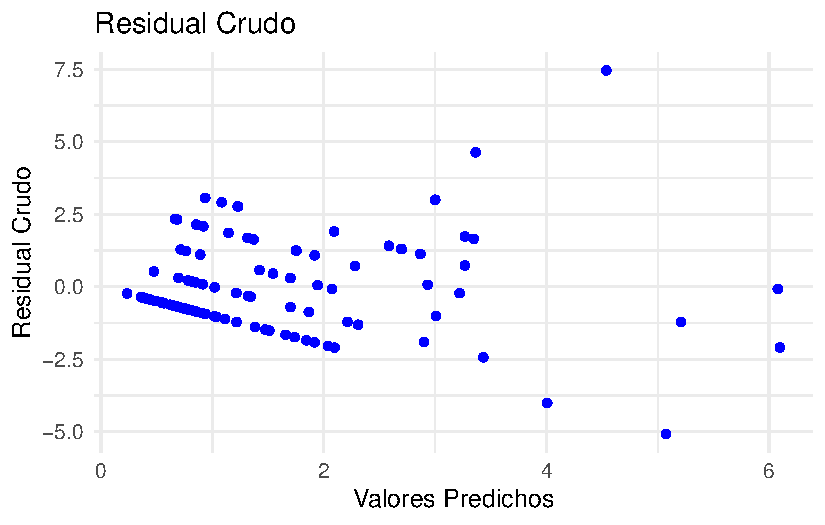
\includegraphics{Modelos_files/figure-pdf/unnamed-chunk-24-1.pdf}\end{minipage}%
%
\begin{minipage}{0.50\linewidth}
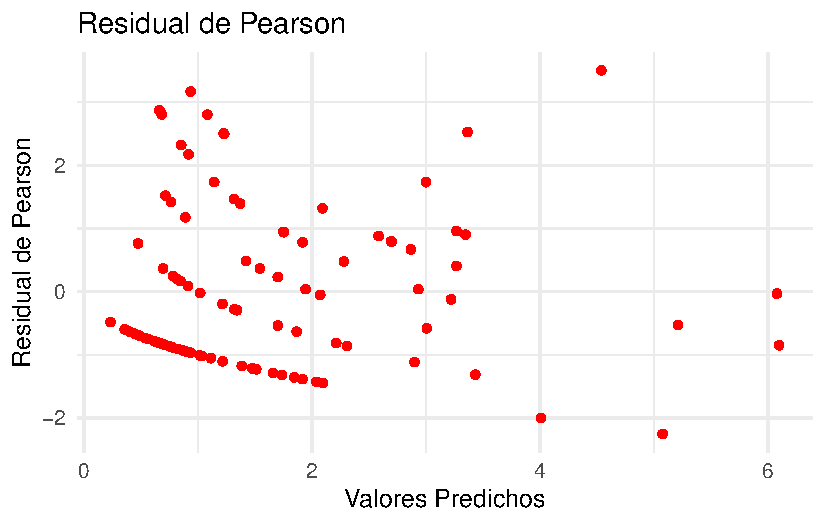
\includegraphics{Modelos_files/figure-pdf/unnamed-chunk-24-2.pdf}\end{minipage}%
\newline
\begin{minipage}{0.50\linewidth}
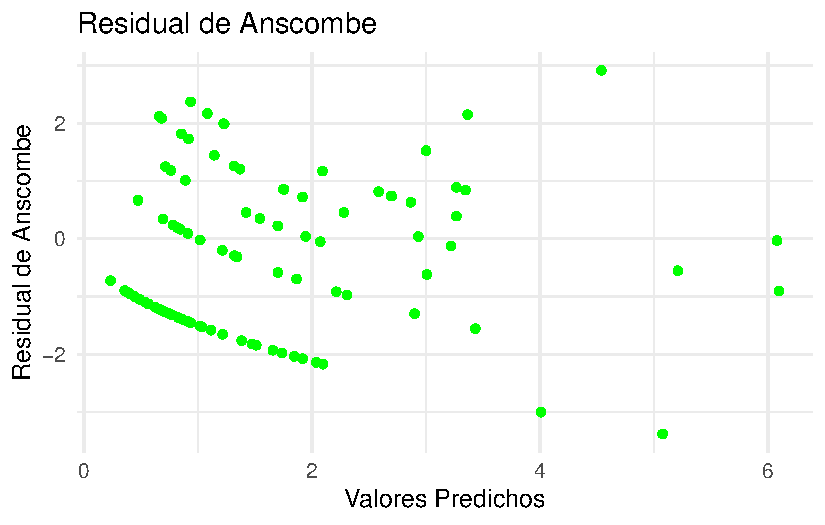
\includegraphics{Modelos_files/figure-pdf/unnamed-chunk-24-3.pdf}\end{minipage}%
%
\begin{minipage}{0.50\linewidth}
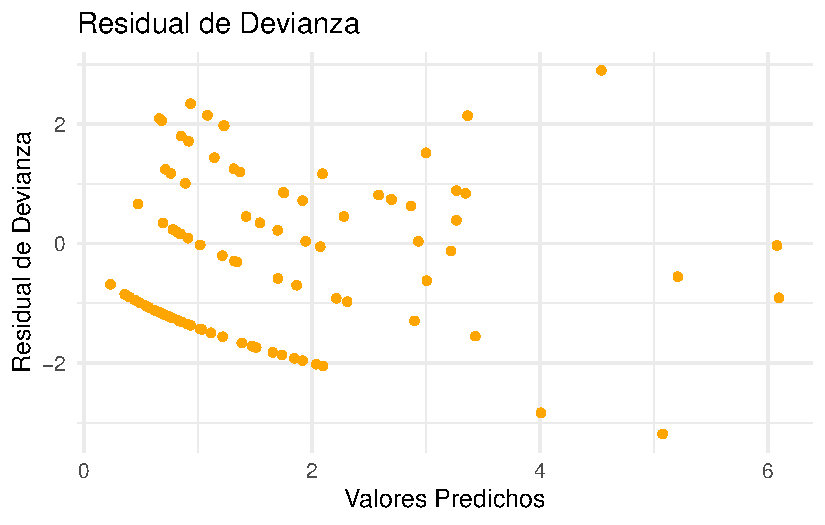
\includegraphics{Modelos_files/figure-pdf/unnamed-chunk-24-4.pdf}\end{minipage}%

\end{figure}%

En todos los casos se puede evidenciar que los residuales presentan un
patrón no aleatorio, esto sugiere que hay presencia de efectos en alguna
de las variables independientes que no ha sido adecuadamente modelada

Además se graficaron los residuales contra las diferentes variables,
para darnos una idea de que podría ser el problema:

\begin{Shaded}
\begin{Highlighting}[]
\CommentTok{\# Gráfico de los residuales crudos contra la variable S}

\NormalTok{c1 }\OtherTok{\textless{}{-}} \FunctionTok{ggplot}\NormalTok{(df\_residuals.c, }\FunctionTok{aes}\NormalTok{(}\AttributeTok{x =}\NormalTok{ S, }\AttributeTok{y =}\NormalTok{ residual)) }\SpecialCharTok{+}
    \FunctionTok{geom\_point}\NormalTok{(}\AttributeTok{color =} \StringTok{\textquotesingle{}blue\textquotesingle{}}\NormalTok{) }\SpecialCharTok{+}
    \FunctionTok{labs}\NormalTok{(}\AttributeTok{title =} \StringTok{\textquotesingle{}Residual Crudo\textquotesingle{}}\NormalTok{, }\AttributeTok{x =} \StringTok{\textquotesingle{}(S)\textquotesingle{}}\NormalTok{, }\AttributeTok{y =} \StringTok{\textquotesingle{}Residual Crudo\textquotesingle{}}\NormalTok{) }\SpecialCharTok{+}
    \FunctionTok{theme\_minimal}\NormalTok{(}\DecValTok{12}\NormalTok{)}

\NormalTok{c2 }\OtherTok{\textless{}{-}} \FunctionTok{ggplot}\NormalTok{(df\_residuals.c, }\FunctionTok{aes}\NormalTok{(}\AttributeTok{x =}\NormalTok{ W, }\AttributeTok{y =}\NormalTok{ residual)) }\SpecialCharTok{+}
    \FunctionTok{geom\_point}\NormalTok{(}\AttributeTok{color =} \StringTok{\textquotesingle{}red\textquotesingle{}}\NormalTok{) }\SpecialCharTok{+}
    \FunctionTok{labs}\NormalTok{(}\AttributeTok{title =} \StringTok{\textquotesingle{}Residual Crudo\textquotesingle{}}\NormalTok{, }\AttributeTok{x =} \StringTok{\textquotesingle{}(W)\textquotesingle{}}\NormalTok{, }\AttributeTok{y =} \StringTok{\textquotesingle{}Residual Crudo\textquotesingle{}}\NormalTok{) }\SpecialCharTok{+}
    \FunctionTok{theme\_minimal}\NormalTok{(}\DecValTok{12}\NormalTok{)}

\NormalTok{c3 }\OtherTok{\textless{}{-}} \FunctionTok{ggplot}\NormalTok{(df\_residuals.c, }\FunctionTok{aes}\NormalTok{(}\AttributeTok{x =}\NormalTok{ Wt, }\AttributeTok{y =}\NormalTok{ residual)) }\SpecialCharTok{+}
    \FunctionTok{geom\_point}\NormalTok{(}\AttributeTok{color =} \StringTok{\textquotesingle{}green\textquotesingle{}}\NormalTok{) }\SpecialCharTok{+}
    \FunctionTok{labs}\NormalTok{(}\AttributeTok{title =} \StringTok{\textquotesingle{}Residual Crudo\textquotesingle{}}\NormalTok{, }\AttributeTok{x =} \StringTok{\textquotesingle{}(Wt)\textquotesingle{}}\NormalTok{, }\AttributeTok{y =} \StringTok{\textquotesingle{}Residual Crudo\textquotesingle{}}\NormalTok{) }\SpecialCharTok{+}
    \FunctionTok{theme\_minimal}\NormalTok{(}\DecValTok{12}\NormalTok{)}

\NormalTok{c4 }\OtherTok{\textless{}{-}} \FunctionTok{ggplot}\NormalTok{(df\_residuals.c, }\FunctionTok{aes}\NormalTok{(}\AttributeTok{x =}\NormalTok{ C, }\AttributeTok{y =}\NormalTok{ residual)) }\SpecialCharTok{+}
    \FunctionTok{geom\_point}\NormalTok{(}\AttributeTok{color =} \StringTok{\textquotesingle{}orange\textquotesingle{}}\NormalTok{) }\SpecialCharTok{+}
    \FunctionTok{labs}\NormalTok{(}\AttributeTok{title =} \StringTok{\textquotesingle{}Residual Crudo\textquotesingle{}}\NormalTok{, }\AttributeTok{x =} \StringTok{\textquotesingle{}(C)\textquotesingle{}}\NormalTok{, }\AttributeTok{y =} \StringTok{\textquotesingle{}Residual Crudo\textquotesingle{}}\NormalTok{) }\SpecialCharTok{+}
    \FunctionTok{theme\_minimal}\NormalTok{(}\DecValTok{12}\NormalTok{)}
\end{Highlighting}
\end{Shaded}

\begin{Shaded}
\begin{Highlighting}[]
\NormalTok{c1; c2; c3; c4}
\end{Highlighting}
\end{Shaded}

\begin{figure}

\begin{minipage}{0.50\linewidth}
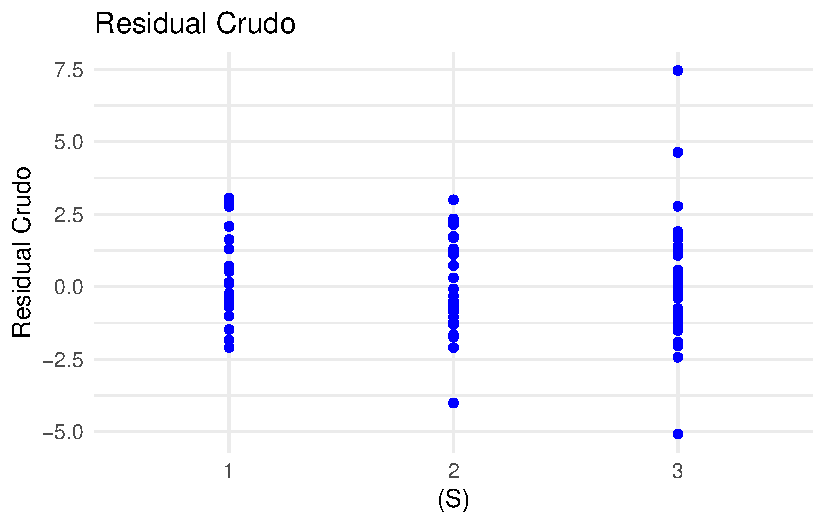
\includegraphics{Modelos_files/figure-pdf/unnamed-chunk-26-1.pdf}\end{minipage}%
%
\begin{minipage}{0.50\linewidth}
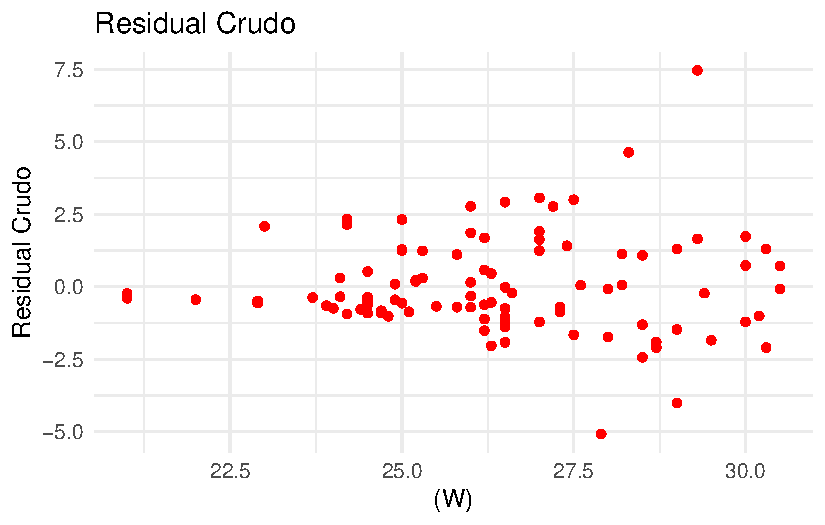
\includegraphics{Modelos_files/figure-pdf/unnamed-chunk-26-2.pdf}\end{minipage}%
\newline
\begin{minipage}{0.50\linewidth}
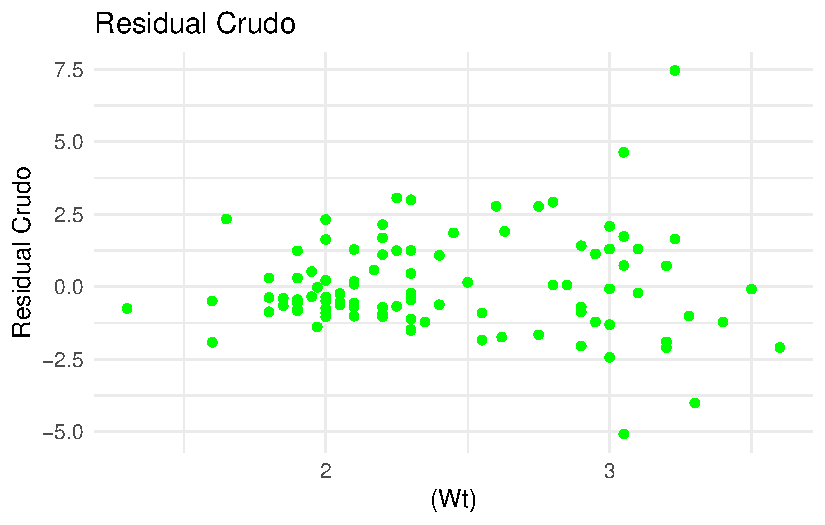
\includegraphics{Modelos_files/figure-pdf/unnamed-chunk-26-3.pdf}\end{minipage}%
%
\begin{minipage}{0.50\linewidth}
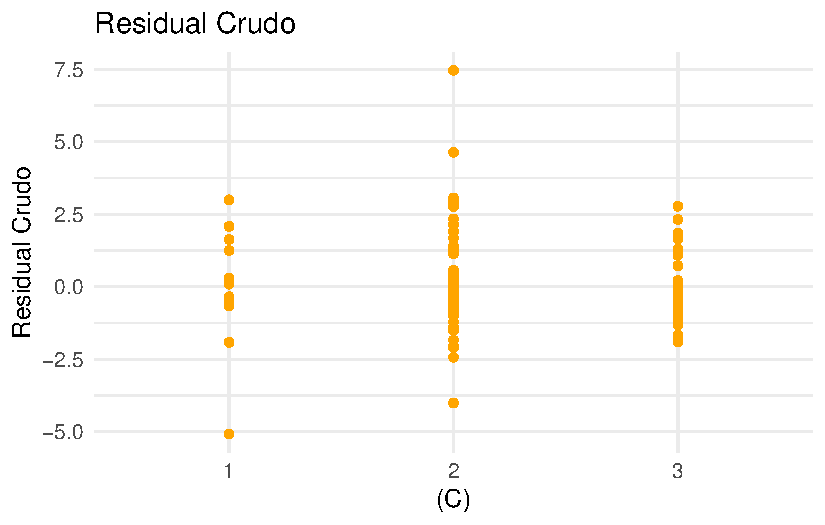
\includegraphics{Modelos_files/figure-pdf/unnamed-chunk-26-4.pdf}\end{minipage}%

\end{figure}%

\begin{Shaded}
\begin{Highlighting}[]
\CommentTok{\# Gráfico de los residuales crudos contra la variable S}

\NormalTok{c1 }\OtherTok{\textless{}{-}} \FunctionTok{ggplot}\NormalTok{(df\_residuals.c, }\FunctionTok{aes}\NormalTok{(}\AttributeTok{x =}\NormalTok{ S, }\AttributeTok{y =}\NormalTok{ residual\_pearson)) }\SpecialCharTok{+}
    \FunctionTok{geom\_point}\NormalTok{(}\AttributeTok{color =} \StringTok{\textquotesingle{}blue\textquotesingle{}}\NormalTok{) }\SpecialCharTok{+}
    \FunctionTok{labs}\NormalTok{(}\AttributeTok{title =} \StringTok{\textquotesingle{}Residual de Pearson\textquotesingle{}}\NormalTok{, }\AttributeTok{x =} \StringTok{\textquotesingle{}(S)\textquotesingle{}}\NormalTok{, }\AttributeTok{y =} \StringTok{\textquotesingle{}Residual de Pearson\textquotesingle{}}\NormalTok{) }\SpecialCharTok{+}
    \FunctionTok{theme\_minimal}\NormalTok{(}\DecValTok{12}\NormalTok{)}

\NormalTok{c2 }\OtherTok{\textless{}{-}} \FunctionTok{ggplot}\NormalTok{(df\_residuals.c, }\FunctionTok{aes}\NormalTok{(}\AttributeTok{x =}\NormalTok{ W, }\AttributeTok{y =}\NormalTok{ residual\_pearson)) }\SpecialCharTok{+}
    \FunctionTok{geom\_point}\NormalTok{(}\AttributeTok{color =} \StringTok{\textquotesingle{}red\textquotesingle{}}\NormalTok{) }\SpecialCharTok{+}
    \FunctionTok{labs}\NormalTok{(}\AttributeTok{title =} \StringTok{\textquotesingle{}Residual de Pearson\textquotesingle{}}\NormalTok{, }\AttributeTok{x =} \StringTok{\textquotesingle{}(W)\textquotesingle{}}\NormalTok{, }\AttributeTok{y =} \StringTok{\textquotesingle{}Residual de Pearson\textquotesingle{}}\NormalTok{) }\SpecialCharTok{+}
    \FunctionTok{theme\_minimal}\NormalTok{(}\DecValTok{12}\NormalTok{)}

\NormalTok{c3 }\OtherTok{\textless{}{-}} \FunctionTok{ggplot}\NormalTok{(df\_residuals.c, }\FunctionTok{aes}\NormalTok{(}\AttributeTok{x =}\NormalTok{ Wt, }\AttributeTok{y =}\NormalTok{ residual\_pearson)) }\SpecialCharTok{+}
    \FunctionTok{geom\_point}\NormalTok{(}\AttributeTok{color =} \StringTok{\textquotesingle{}green\textquotesingle{}}\NormalTok{) }\SpecialCharTok{+}
    \FunctionTok{labs}\NormalTok{(}\AttributeTok{title =} \StringTok{\textquotesingle{}Residual de Pearson\textquotesingle{}}\NormalTok{, }\AttributeTok{x =} \StringTok{\textquotesingle{}(Wt)\textquotesingle{}}\NormalTok{, }\AttributeTok{y =} \StringTok{\textquotesingle{}Residual de Pearson\textquotesingle{}}\NormalTok{) }\SpecialCharTok{+}
    \FunctionTok{theme\_minimal}\NormalTok{(}\DecValTok{12}\NormalTok{)}

\NormalTok{c4 }\OtherTok{\textless{}{-}} \FunctionTok{ggplot}\NormalTok{(df\_residuals.c, }\FunctionTok{aes}\NormalTok{(}\AttributeTok{x =}\NormalTok{ C, }\AttributeTok{y =}\NormalTok{ residual\_pearson)) }\SpecialCharTok{+}
    \FunctionTok{geom\_point}\NormalTok{(}\AttributeTok{color =} \StringTok{\textquotesingle{}orange\textquotesingle{}}\NormalTok{) }\SpecialCharTok{+}
    \FunctionTok{labs}\NormalTok{(}\AttributeTok{title =} \StringTok{\textquotesingle{}Residual de Pearson\textquotesingle{}}\NormalTok{, }\AttributeTok{x =} \StringTok{\textquotesingle{}(C)\textquotesingle{}}\NormalTok{, }\AttributeTok{y =} \StringTok{\textquotesingle{}Residual de Pearson\textquotesingle{}}\NormalTok{) }\SpecialCharTok{+}
    \FunctionTok{theme\_minimal}\NormalTok{(}\DecValTok{12}\NormalTok{)}
\end{Highlighting}
\end{Shaded}

\begin{Shaded}
\begin{Highlighting}[]
\NormalTok{c1; c2; c3; c4}
\end{Highlighting}
\end{Shaded}

\begin{figure}

\begin{minipage}{0.50\linewidth}
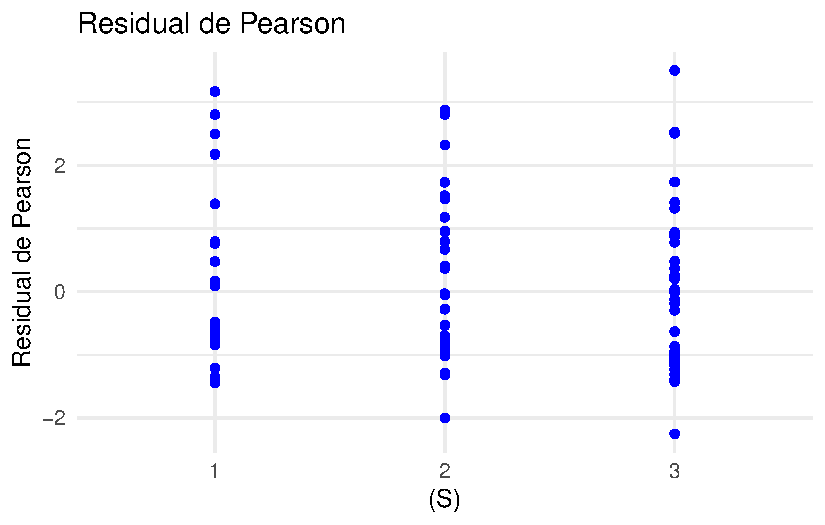
\includegraphics{Modelos_files/figure-pdf/unnamed-chunk-28-1.pdf}\end{minipage}%
%
\begin{minipage}{0.50\linewidth}
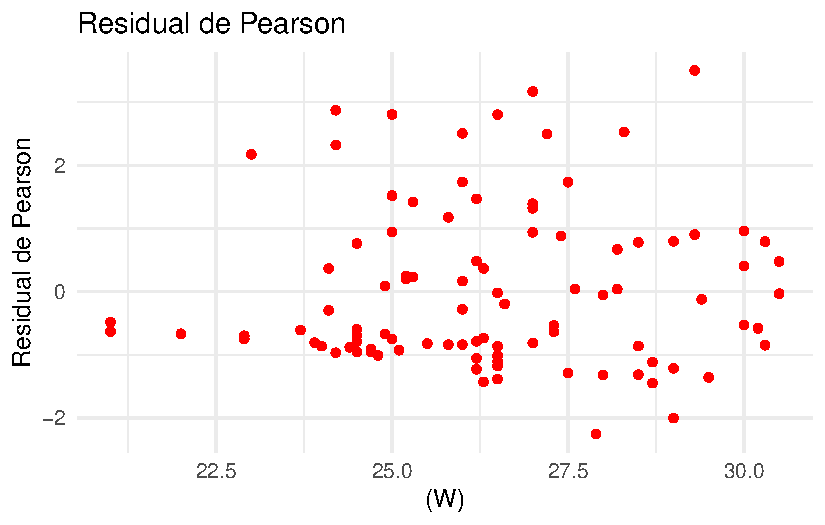
\includegraphics{Modelos_files/figure-pdf/unnamed-chunk-28-2.pdf}\end{minipage}%
\newline
\begin{minipage}{0.50\linewidth}
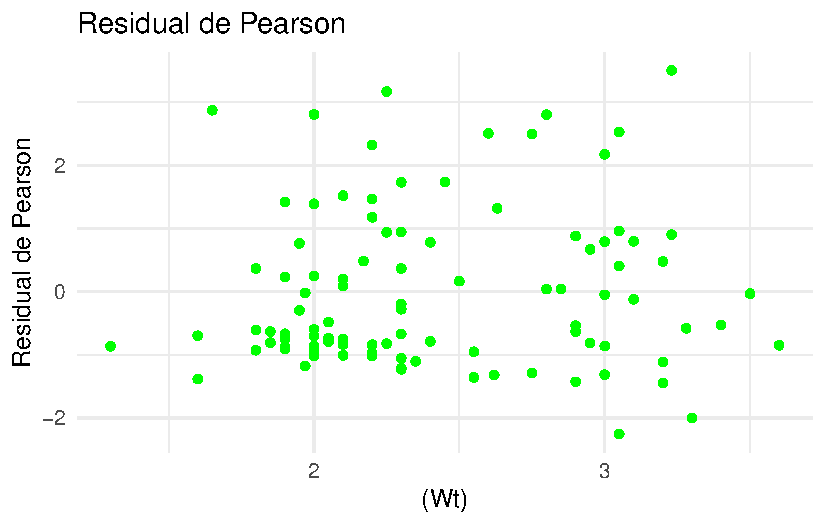
\includegraphics{Modelos_files/figure-pdf/unnamed-chunk-28-3.pdf}\end{minipage}%
%
\begin{minipage}{0.50\linewidth}
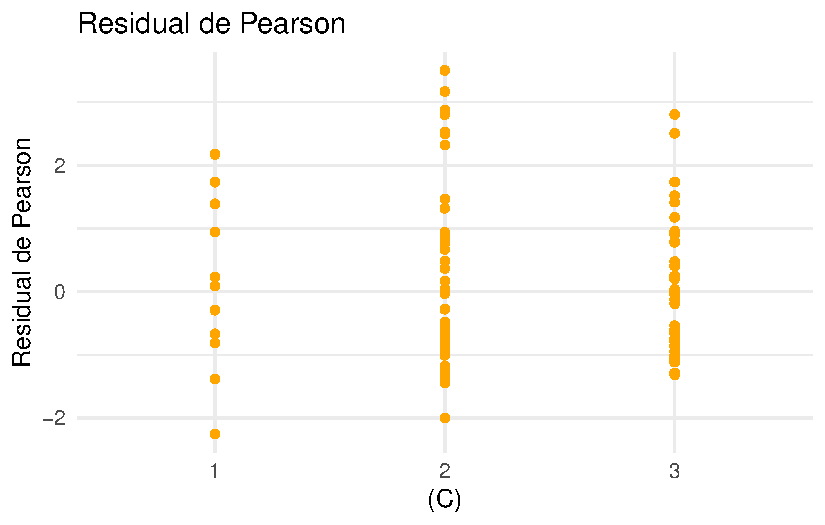
\includegraphics{Modelos_files/figure-pdf/unnamed-chunk-28-4.pdf}\end{minipage}%

\end{figure}%

\begin{Shaded}
\begin{Highlighting}[]
\CommentTok{\# Gráfico de los residuales crudos contra la variable S}

\NormalTok{c1 }\OtherTok{\textless{}{-}} \FunctionTok{ggplot}\NormalTok{(df\_residuals.c, }\FunctionTok{aes}\NormalTok{(}\AttributeTok{x =}\NormalTok{ S, }\AttributeTok{y =}\NormalTok{ residual\_anscombe)) }\SpecialCharTok{+}
    \FunctionTok{geom\_point}\NormalTok{(}\AttributeTok{color =} \StringTok{\textquotesingle{}blue\textquotesingle{}}\NormalTok{) }\SpecialCharTok{+}
    \FunctionTok{labs}\NormalTok{(}\AttributeTok{title =} \StringTok{\textquotesingle{}Residual de Anscombe\textquotesingle{}}\NormalTok{, }\AttributeTok{x =} \StringTok{\textquotesingle{}(S)\textquotesingle{}}\NormalTok{, }\AttributeTok{y =} \StringTok{\textquotesingle{}Residual de Anscombe\textquotesingle{}}\NormalTok{) }\SpecialCharTok{+}
    \FunctionTok{theme\_minimal}\NormalTok{(}\DecValTok{12}\NormalTok{)}

\NormalTok{c2 }\OtherTok{\textless{}{-}} \FunctionTok{ggplot}\NormalTok{(df\_residuals.c, }\FunctionTok{aes}\NormalTok{(}\AttributeTok{x =}\NormalTok{ W, }\AttributeTok{y =}\NormalTok{ residual\_anscombe)) }\SpecialCharTok{+}
    \FunctionTok{geom\_point}\NormalTok{(}\AttributeTok{color =} \StringTok{\textquotesingle{}red\textquotesingle{}}\NormalTok{) }\SpecialCharTok{+}
    \FunctionTok{labs}\NormalTok{(}\AttributeTok{title =} \StringTok{\textquotesingle{}Residual de Anscombe\textquotesingle{}}\NormalTok{, }\AttributeTok{x =} \StringTok{\textquotesingle{}(W)\textquotesingle{}}\NormalTok{, }\AttributeTok{y =} \StringTok{\textquotesingle{}Residual de Anscombe\textquotesingle{}}\NormalTok{) }\SpecialCharTok{+}
    \FunctionTok{theme\_minimal}\NormalTok{(}\DecValTok{12}\NormalTok{)}

\NormalTok{c3 }\OtherTok{\textless{}{-}} \FunctionTok{ggplot}\NormalTok{(df\_residuals.c, }\FunctionTok{aes}\NormalTok{(}\AttributeTok{x =}\NormalTok{ Wt, }\AttributeTok{y =}\NormalTok{ residual\_anscombe)) }\SpecialCharTok{+}
    \FunctionTok{geom\_point}\NormalTok{(}\AttributeTok{color =} \StringTok{\textquotesingle{}green\textquotesingle{}}\NormalTok{) }\SpecialCharTok{+}
    \FunctionTok{labs}\NormalTok{(}\AttributeTok{title =} \StringTok{\textquotesingle{}Residual de Anscombe\textquotesingle{}}\NormalTok{, }\AttributeTok{x =} \StringTok{\textquotesingle{}(Wt)\textquotesingle{}}\NormalTok{, }\AttributeTok{y =} \StringTok{\textquotesingle{}Residual de Anscombe\textquotesingle{}}\NormalTok{) }\SpecialCharTok{+}
    \FunctionTok{theme\_minimal}\NormalTok{(}\DecValTok{12}\NormalTok{)}

\NormalTok{c4 }\OtherTok{\textless{}{-}} \FunctionTok{ggplot}\NormalTok{(df\_residuals.c, }\FunctionTok{aes}\NormalTok{(}\AttributeTok{x =}\NormalTok{ C, }\AttributeTok{y =}\NormalTok{ residual\_anscombe)) }\SpecialCharTok{+}
    \FunctionTok{geom\_point}\NormalTok{(}\AttributeTok{color =} \StringTok{\textquotesingle{}orange\textquotesingle{}}\NormalTok{) }\SpecialCharTok{+}
    \FunctionTok{labs}\NormalTok{(}\AttributeTok{title =} \StringTok{\textquotesingle{}Residual de Anscombe\textquotesingle{}}\NormalTok{, }\AttributeTok{x =} \StringTok{\textquotesingle{}(C)\textquotesingle{}}\NormalTok{, }\AttributeTok{y =} \StringTok{\textquotesingle{}Residual de Anscombe\textquotesingle{}}\NormalTok{) }\SpecialCharTok{+}
    \FunctionTok{theme\_minimal}\NormalTok{(}\DecValTok{12}\NormalTok{)}
\end{Highlighting}
\end{Shaded}

\begin{Shaded}
\begin{Highlighting}[]
\NormalTok{c1; c2; c3; c4}
\end{Highlighting}
\end{Shaded}

\begin{figure}

\begin{minipage}{0.50\linewidth}
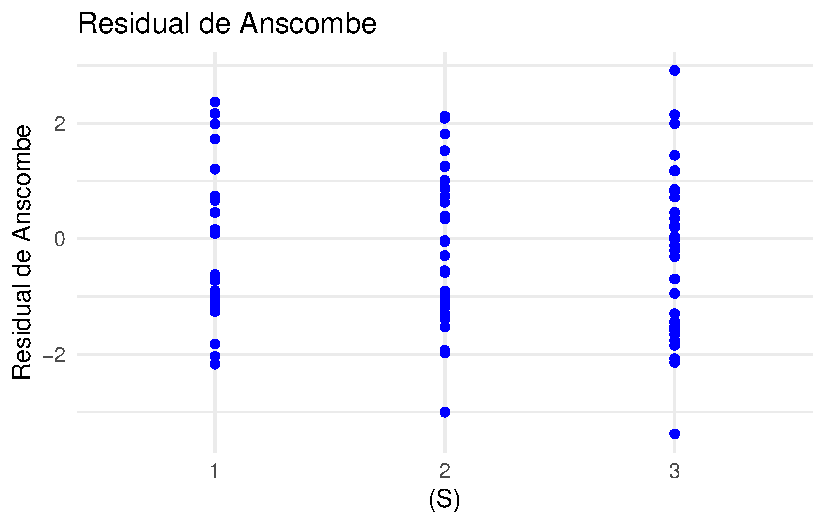
\includegraphics{Modelos_files/figure-pdf/unnamed-chunk-30-1.pdf}\end{minipage}%
%
\begin{minipage}{0.50\linewidth}
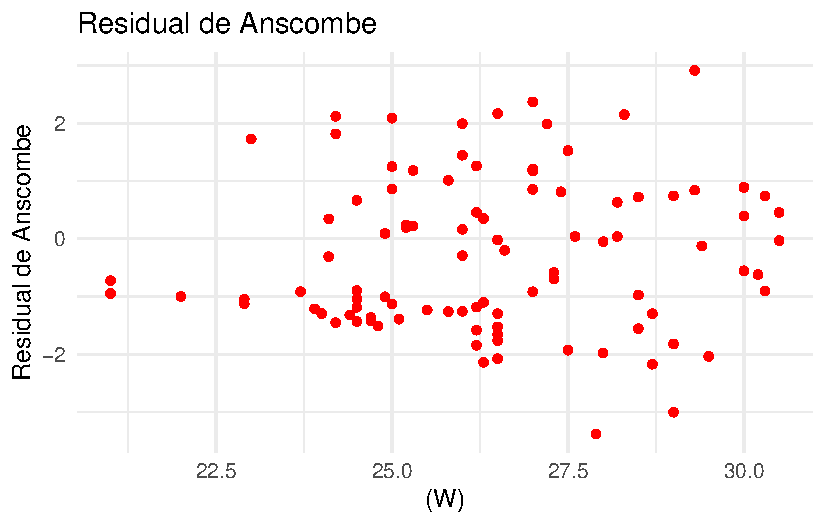
\includegraphics{Modelos_files/figure-pdf/unnamed-chunk-30-2.pdf}\end{minipage}%
\newline
\begin{minipage}{0.50\linewidth}
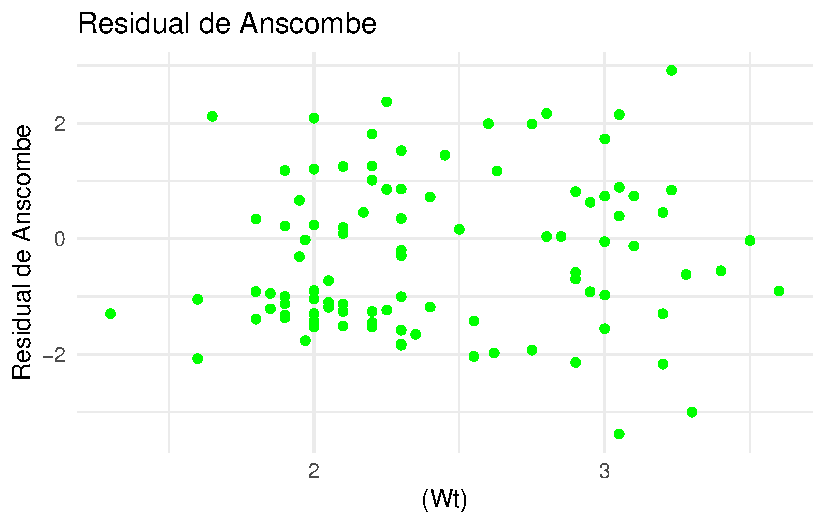
\includegraphics{Modelos_files/figure-pdf/unnamed-chunk-30-3.pdf}\end{minipage}%
%
\begin{minipage}{0.50\linewidth}
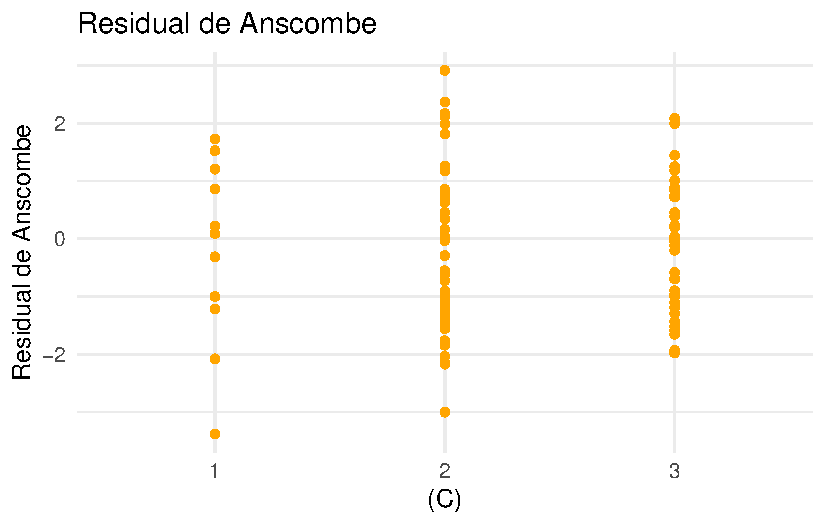
\includegraphics{Modelos_files/figure-pdf/unnamed-chunk-30-4.pdf}\end{minipage}%

\end{figure}%

\begin{Shaded}
\begin{Highlighting}[]
\CommentTok{\# Gráfico de los residuales crudos contra la variable S}

\NormalTok{c1 }\OtherTok{\textless{}{-}} \FunctionTok{ggplot}\NormalTok{(df\_residuals.c, }\FunctionTok{aes}\NormalTok{(}\AttributeTok{x =}\NormalTok{ S, }\AttributeTok{y =}\NormalTok{ residual\_deviance)) }\SpecialCharTok{+}
    \FunctionTok{geom\_point}\NormalTok{(}\AttributeTok{color =} \StringTok{\textquotesingle{}blue\textquotesingle{}}\NormalTok{) }\SpecialCharTok{+}
    \FunctionTok{labs}\NormalTok{(}\AttributeTok{title =} \StringTok{\textquotesingle{}Residual de Devianza\textquotesingle{}}\NormalTok{, }\AttributeTok{x =} \StringTok{\textquotesingle{}(S)\textquotesingle{}}\NormalTok{, }\AttributeTok{y =} \StringTok{\textquotesingle{}Residual de Devianza\textquotesingle{}}\NormalTok{) }\SpecialCharTok{+}
    \FunctionTok{theme\_minimal}\NormalTok{(}\DecValTok{12}\NormalTok{)}

\NormalTok{c2 }\OtherTok{\textless{}{-}} \FunctionTok{ggplot}\NormalTok{(df\_residuals.c, }\FunctionTok{aes}\NormalTok{(}\AttributeTok{x =}\NormalTok{ W, }\AttributeTok{y =}\NormalTok{ residual\_deviance)) }\SpecialCharTok{+}
    \FunctionTok{geom\_point}\NormalTok{(}\AttributeTok{color =} \StringTok{\textquotesingle{}red\textquotesingle{}}\NormalTok{) }\SpecialCharTok{+}
    \FunctionTok{labs}\NormalTok{(}\AttributeTok{title =} \StringTok{\textquotesingle{}Residual de Devianza\textquotesingle{}}\NormalTok{, }\AttributeTok{x =} \StringTok{\textquotesingle{}(W)\textquotesingle{}}\NormalTok{, }\AttributeTok{y =} \StringTok{\textquotesingle{}Residual de Devianza\textquotesingle{}}\NormalTok{) }\SpecialCharTok{+}
    \FunctionTok{theme\_minimal}\NormalTok{(}\DecValTok{12}\NormalTok{)}

\NormalTok{c3 }\OtherTok{\textless{}{-}} \FunctionTok{ggplot}\NormalTok{(df\_residuals.c, }\FunctionTok{aes}\NormalTok{(}\AttributeTok{x =}\NormalTok{ Wt, }\AttributeTok{y =}\NormalTok{ residual\_deviance)) }\SpecialCharTok{+}
    \FunctionTok{geom\_point}\NormalTok{(}\AttributeTok{color =} \StringTok{\textquotesingle{}green\textquotesingle{}}\NormalTok{) }\SpecialCharTok{+}
    \FunctionTok{labs}\NormalTok{(}\AttributeTok{title =} \StringTok{\textquotesingle{}Residual de Devianza\textquotesingle{}}\NormalTok{, }\AttributeTok{x =} \StringTok{\textquotesingle{}(Wt)\textquotesingle{}}\NormalTok{, }\AttributeTok{y =} \StringTok{\textquotesingle{}Residual de Devianza\textquotesingle{}}\NormalTok{) }\SpecialCharTok{+}
    \FunctionTok{theme\_minimal}\NormalTok{(}\DecValTok{12}\NormalTok{)}

\NormalTok{c4 }\OtherTok{\textless{}{-}} \FunctionTok{ggplot}\NormalTok{(df\_residuals.c, }\FunctionTok{aes}\NormalTok{(}\AttributeTok{x =}\NormalTok{ C, }\AttributeTok{y =}\NormalTok{ residual\_deviance)) }\SpecialCharTok{+}
    \FunctionTok{geom\_point}\NormalTok{(}\AttributeTok{color =} \StringTok{\textquotesingle{}orange\textquotesingle{}}\NormalTok{) }\SpecialCharTok{+}
    \FunctionTok{labs}\NormalTok{(}\AttributeTok{title =} \StringTok{\textquotesingle{}Residual de Devianza\textquotesingle{}}\NormalTok{, }\AttributeTok{x =} \StringTok{\textquotesingle{}(C)\textquotesingle{}}\NormalTok{, }\AttributeTok{y =} \StringTok{\textquotesingle{}Residual de Devianza\textquotesingle{}}\NormalTok{) }\SpecialCharTok{+}
    \FunctionTok{theme\_minimal}\NormalTok{(}\DecValTok{12}\NormalTok{)}
\end{Highlighting}
\end{Shaded}

\begin{Shaded}
\begin{Highlighting}[]
\NormalTok{c1; c2; c3; c4}
\end{Highlighting}
\end{Shaded}

\begin{figure}

\begin{minipage}{0.50\linewidth}
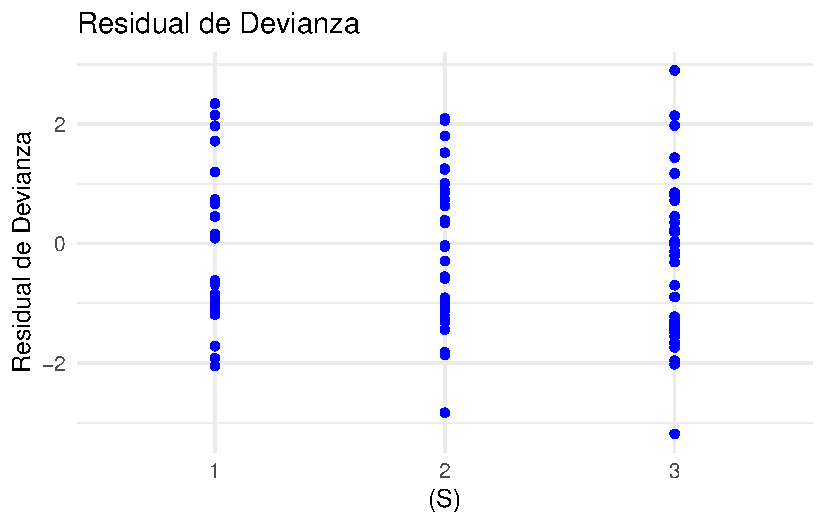
\includegraphics{Modelos_files/figure-pdf/unnamed-chunk-32-1.pdf}\end{minipage}%
%
\begin{minipage}{0.50\linewidth}
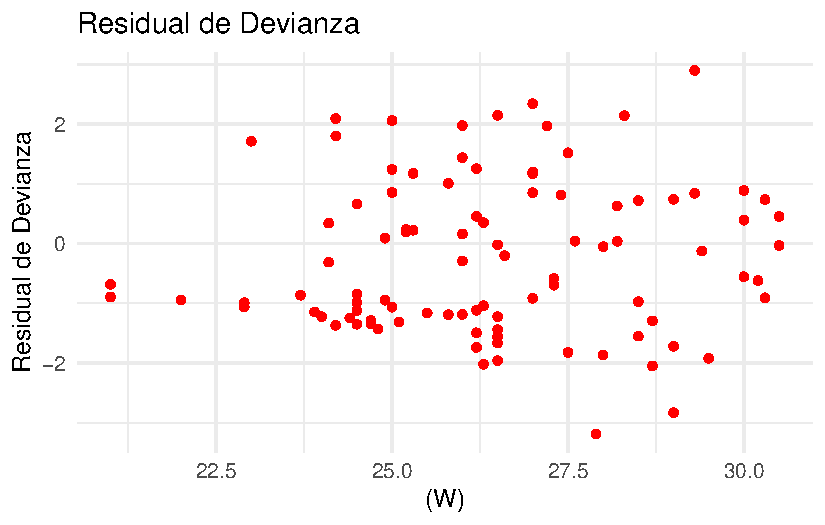
\includegraphics{Modelos_files/figure-pdf/unnamed-chunk-32-2.pdf}\end{minipage}%
\newline
\begin{minipage}{0.50\linewidth}
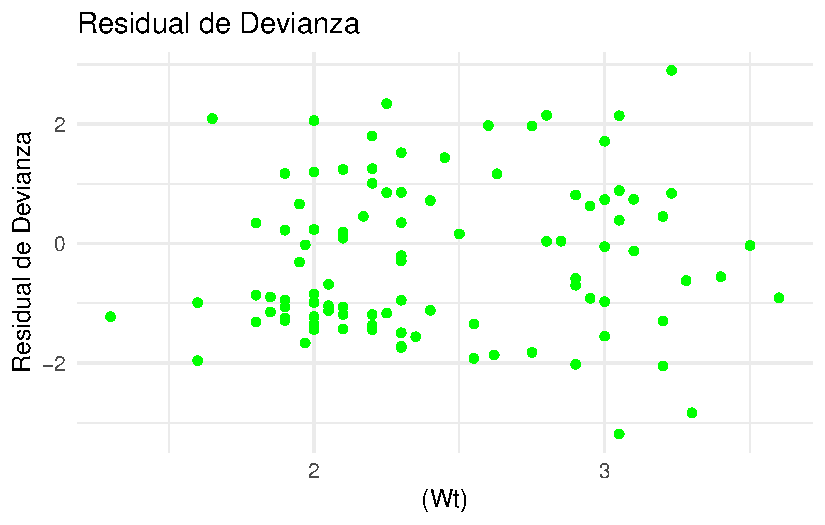
\includegraphics{Modelos_files/figure-pdf/unnamed-chunk-32-3.pdf}\end{minipage}%
%
\begin{minipage}{0.50\linewidth}
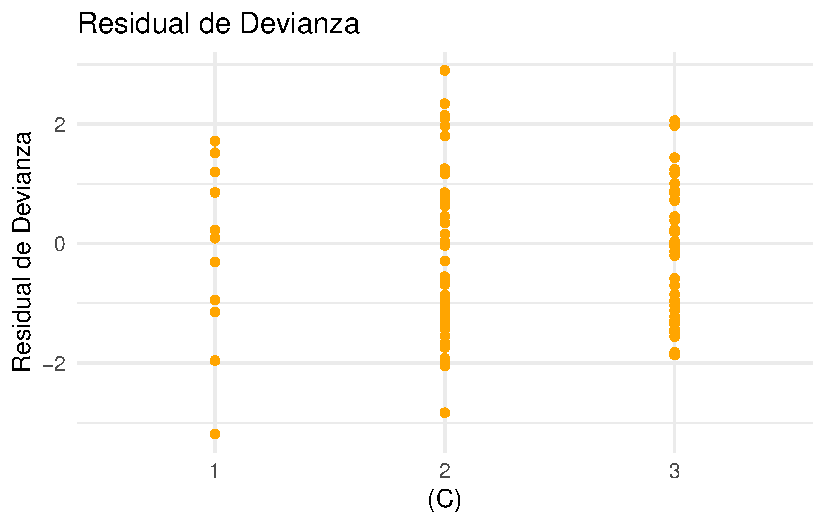
\includegraphics{Modelos_files/figure-pdf/unnamed-chunk-32-4.pdf}\end{minipage}%

\end{figure}%

En los gráficos de los distintos residuales frente a las variables se
puede ver que las variables de ancho y peso parecen estar bien
modeladas, mientras que las variables categóricas de la condición de la
espina y el color pueden estar necesitando interacciones.

\begin{Shaded}
\begin{Highlighting}[]
\NormalTok{X\_completa }\OtherTok{\textless{}{-}} \FunctionTok{model.matrix}\NormalTok{(Sa}
  \SpecialCharTok{\textasciitilde{}}\NormalTok{ C }\SpecialCharTok{+}\NormalTok{ S }\SpecialCharTok{+}\NormalTok{ W }\SpecialCharTok{+}\NormalTok{ Wt }\SpecialCharTok{+}
\NormalTok{    C}\SpecialCharTok{:}\NormalTok{S }\SpecialCharTok{+}\NormalTok{ C}\SpecialCharTok{:}\NormalTok{W }\SpecialCharTok{+}\NormalTok{ C}\SpecialCharTok{:}\NormalTok{Wt }\SpecialCharTok{+}
\NormalTok{    S}\SpecialCharTok{:}\NormalTok{W }\SpecialCharTok{+}\NormalTok{ S}\SpecialCharTok{:}\NormalTok{Wt,}
  \AttributeTok{data =}\NormalTok{ crabs}
\NormalTok{)}

\CommentTok{\# Ajustar modelo con Fisher Scoring}
\NormalTok{modelos\_crangrejos\_interactions }\OtherTok{\textless{}{-}} \FunctionTok{fisher\_scoring\_poisson}\NormalTok{(}
\NormalTok{  crabs[,}\DecValTok{5}\NormalTok{],}
  \AttributeTok{X =}\NormalTok{ X\_completa,}
  \AttributeTok{beta\_init =} \FunctionTok{c}\NormalTok{(}\FunctionTok{log}\NormalTok{(}\FunctionTok{mean}\NormalTok{(crabs[,}\DecValTok{5}\NormalTok{])), }\FunctionTok{rep}\NormalTok{(}\DecValTok{0}\NormalTok{, }\FunctionTok{ncol}\NormalTok{(X\_completa)}\SpecialCharTok{{-}}\DecValTok{1}\NormalTok{)}
\NormalTok{))}
\end{Highlighting}
\end{Shaded}

\begin{verbatim}
El algoritmo convergió en la iteración 7
\end{verbatim}

\begin{Shaded}
\begin{Highlighting}[]
\CommentTok{\# Nombres para los coeficientes (incluyendo términos de interacción)}
\FunctionTok{names}\NormalTok{(modelos\_crangrejos\_interactions}\SpecialCharTok{$}\NormalTok{beta) }\OtherTok{\textless{}{-}} \FunctionTok{colnames}\NormalTok{(X\_completa)}
\NormalTok{modelos\_crangrejos\_interactions}\SpecialCharTok{$}\NormalTok{beta}
\end{Highlighting}
\end{Shaded}

\begin{verbatim}
(Intercept)          C2          C3          S2          S3           W 
-1.95263232 -5.88591899 -4.40931107 -2.75579242 -5.40619991  0.03903109 
         Wt       C2:S2       C3:S2       C2:S3       C3:S3        C2:W 
 0.58667464 -0.01213212  0.25629744  1.54090159  1.54075734  0.14599903 
       C3:W       C2:Wt       C3:Wt        S2:W        S3:W       S2:Wt 
 0.08503343  0.48579785  0.37351649  0.30830437  0.22286260 -1.88949419 
      S3:Wt 
-0.49629809 
\end{verbatim}

\begin{Shaded}
\begin{Highlighting}[]
\NormalTok{modelo\_cangre\_completo\_glm }\OtherTok{\textless{}{-}} \FunctionTok{glm}\NormalTok{(Sa}
  \SpecialCharTok{\textasciitilde{}}\NormalTok{ C }\SpecialCharTok{+}\NormalTok{ S }\SpecialCharTok{+}\NormalTok{ W }\SpecialCharTok{+}\NormalTok{ Wt }\SpecialCharTok{+}
\NormalTok{    C}\SpecialCharTok{:}\NormalTok{S }\SpecialCharTok{+}\NormalTok{ C}\SpecialCharTok{:}\NormalTok{W }\SpecialCharTok{+}\NormalTok{ C}\SpecialCharTok{:}\NormalTok{Wt }\SpecialCharTok{+}
\NormalTok{    S}\SpecialCharTok{:}\NormalTok{W }\SpecialCharTok{+}\NormalTok{ S}\SpecialCharTok{:}\NormalTok{Wt,}
  \AttributeTok{data =}\NormalTok{ crabs,}
\AttributeTok{family =} \FunctionTok{poisson}\NormalTok{(}\AttributeTok{link =} \StringTok{"log"}\NormalTok{))}

\FunctionTok{names}\NormalTok{(modelo\_cangre\_completo\_glm}\SpecialCharTok{$}\NormalTok{coefficients) }\OtherTok{\textless{}{-}} \FunctionTok{names}\NormalTok{(modelos\_crangrejos\_interactions}\SpecialCharTok{$}\NormalTok{beta)}
\NormalTok{modelo\_cangre\_completo\_glm}\SpecialCharTok{$}\NormalTok{coefficients}
\end{Highlighting}
\end{Shaded}

\begin{verbatim}
(Intercept)          C2          C3          S2          S3           W 
-1.95263254 -5.88591879 -4.40931091 -2.75579238 -5.40619982  0.03903110 
         Wt       C2:S2       C3:S2       C2:S3       C3:S3        C2:W 
 0.58667468 -0.01213211  0.25629746  1.54090153  1.54075729  0.14599903 
       C3:W       C2:Wt       C3:Wt        S2:W        S3:W       S2:Wt 
 0.08503343  0.48579780  0.37351643  0.30830437  0.22286260 -1.88949416 
      S3:Wt 
-0.49629806 
\end{verbatim}

En la siguiente tabla se puede evidenciar los resultados de ambos
métodos: En la siguiente tabla se puede ver la comparación con ambos
métodos:

\begin{longtable}[]{@{}
  >{\raggedright\arraybackslash}p{(\columnwidth - 4\tabcolsep) * \real{0.2059}}
  >{\centering\arraybackslash}p{(\columnwidth - 4\tabcolsep) * \real{0.4265}}
  >{\centering\arraybackslash}p{(\columnwidth - 4\tabcolsep) * \real{0.3676}}@{}}
\toprule\noalign{}
\begin{minipage}[b]{\linewidth}\raggedright
Variable
\end{minipage} & \begin{minipage}[b]{\linewidth}\centering
fisher\_scoring\_poisson
\end{minipage} & \begin{minipage}[b]{\linewidth}\centering
glm
\end{minipage} \\
\midrule\noalign{}
\endhead
\bottomrule\noalign{}
\endlastfoot
(Intercept) & \(\hat{\beta}_0 = -6.4407728\) &
\(\hat{\beta}_0 = -6.4407727\) \\
C2 & \(\hat{\beta}_1 = -0.4973794\) & \(\hat{\beta}_1 = -0.4973794\) \\
C3 & \(\hat{\beta}_2 = -0.8020200\) & \(\hat{\beta}_2 = -0.8020200\) \\
S2 & \(\hat{\beta}_3 = 0.5369707\) & \(\hat{\beta}_3 = 0.5369707\) \\
S3 & \(\hat{\beta}_4 = 0.6290147\) & \(\hat{\beta}_4 = 0.6290147\) \\
W & \(\hat{\beta}_5 = 0.2159377\) & \(\hat{\beta}_5 = 0.2159377\) \\
Wt & \(\hat{\beta}_6 = 0.4628472\) & \(\hat{\beta}_6 = 0.4628472\) \\
C2 & \(\hat{\beta}_7 = -0.4973794\) & \(\hat{\beta}_1 = -0.4973794\) \\
C3 & \(\hat{\beta}_8 = -0.8020200\) & \(\hat{\beta}_2 = -0.8020200\) \\
C2 & \(\hat{\beta}_9 = -0.4973794\) & \(\hat{\beta}_1 = -0.4973794\) \\
C3 & \(\hat{\beta}_10 = -0.8020200\) & \(\hat{\beta}_2 = -0.8020200\) \\
C2 & \(\hat{\beta}_11 = -0.4973794\) & \(\hat{\beta}_1 = -0.4973794\) \\
C3 & \(\hat{\beta}_12 = -0.8020200\) & \(\hat{\beta}_2 = -0.8020200\) \\
C2 & \(\hat{\beta}_13 = -0.4973794\) & \(\hat{\beta}_1 = -0.4973794\) \\
C3 & \(\hat{\beta}_14 = -0.8020200\) & \(\hat{\beta}_2 = -0.8020200\) \\
S2 & \(\hat{\beta}_15 = 0.5369707\) & \(\hat{\beta}_3 = 0.5369707\) \\
S3 & \(\hat{\beta}_16 = 0.6290147\) & \(\hat{\beta}_4 = 0.6290147\) \\
S2 & \(\hat{\beta}_17 = 0.5369707\) & \(\hat{\beta}_3 = 0.5369707\) \\
S3 & \(\hat{\beta}_18= 0.6290147\) & \(\hat{\beta}_4 = 0.6290147\) \\
S2 & \(\hat{\beta}_19 = 0.5369707\) & \(\hat{\beta}_3 = 0.5369707\) \\
S3 & \(\hat{\beta}_20 = 0.6290147\) & \(\hat{\beta}_4 = 0.6290147\) \\
S2 & \(\hat{\beta}_21 = 0.5369707\) & \(\hat{\beta}_3 = 0.5369707\) \\
S3 & \(\hat{\beta}_22 = 0.6290147\) & \(\hat{\beta}_4 = 0.6290147\) \\
\end{longtable}

\begin{Shaded}
\begin{Highlighting}[]
\NormalTok{df\_residuals.c.interac }\OtherTok{\textless{}{-}} \FunctionTok{data.frame}\NormalTok{(}
    \AttributeTok{C=}\NormalTok{crabs}\SpecialCharTok{$}\NormalTok{C,}
    \AttributeTok{S=}\NormalTok{crabs}\SpecialCharTok{$}\NormalTok{S,}
    \AttributeTok{W=}\NormalTok{crabs}\SpecialCharTok{$}\NormalTok{W,}
    \AttributeTok{Wt=}\NormalTok{crabs}\SpecialCharTok{$}\NormalTok{Wt,}
    \AttributeTok{predichos =}\NormalTok{ modelos\_crangrejos\_interactions}\SpecialCharTok{$}\NormalTok{predichos,}
    \AttributeTok{residual =}\NormalTok{ modelos\_crangrejos\_interactions}\SpecialCharTok{$}\NormalTok{residual,}
    \AttributeTok{residual\_pearson =}\NormalTok{ modelos\_crangrejos\_interactions}\SpecialCharTok{$}\NormalTok{residual\_pearson,}
    \AttributeTok{residual\_anscombe =}\NormalTok{ modelos\_crangrejos\_interactions}\SpecialCharTok{$}\NormalTok{residual\_anscombe,}
    \AttributeTok{residual\_deviance =}\NormalTok{ modelos\_crangrejos\_interactions}\SpecialCharTok{$}\NormalTok{residual\_deviance}
\NormalTok{  )}
\end{Highlighting}
\end{Shaded}

\begin{Shaded}
\begin{Highlighting}[]
\CommentTok{\# Gráfico de los tres tipos de residuales}

\NormalTok{c1 }\OtherTok{\textless{}{-}} \FunctionTok{ggplot}\NormalTok{(df\_residuals.c.interac, }\FunctionTok{aes}\NormalTok{(}\AttributeTok{x =}\NormalTok{ predichos, }\AttributeTok{y =}\NormalTok{ residual)) }\SpecialCharTok{+}
    \FunctionTok{geom\_point}\NormalTok{(}\AttributeTok{color =} \StringTok{\textquotesingle{}blue\textquotesingle{}}\NormalTok{) }\SpecialCharTok{+}
    \FunctionTok{labs}\NormalTok{(}\AttributeTok{title =} \StringTok{\textquotesingle{}Residual Crudo\textquotesingle{}}\NormalTok{, }\AttributeTok{x =} \StringTok{\textquotesingle{}Valores Predichos\textquotesingle{}}\NormalTok{, }\AttributeTok{y =} \StringTok{\textquotesingle{}Residual Crudo\textquotesingle{}}\NormalTok{) }\SpecialCharTok{+}
    \FunctionTok{theme\_minimal}\NormalTok{(}\DecValTok{12}\NormalTok{)}

\NormalTok{c2 }\OtherTok{\textless{}{-}} \FunctionTok{ggplot}\NormalTok{(df\_residuals.c.interac, }\FunctionTok{aes}\NormalTok{(}\AttributeTok{x =}\NormalTok{ predichos, }\AttributeTok{y =}\NormalTok{ residual\_pearson)) }\SpecialCharTok{+}
    \FunctionTok{geom\_point}\NormalTok{(}\AttributeTok{color =} \StringTok{\textquotesingle{}red\textquotesingle{}}\NormalTok{) }\SpecialCharTok{+}
    \FunctionTok{labs}\NormalTok{(}\AttributeTok{title =} \StringTok{\textquotesingle{}Residual de Pearson\textquotesingle{}}\NormalTok{, }\AttributeTok{x =} \StringTok{\textquotesingle{}Valores Predichos\textquotesingle{}}\NormalTok{, }\AttributeTok{y =} \StringTok{\textquotesingle{}Residual de Pearson\textquotesingle{}}\NormalTok{) }\SpecialCharTok{+}
    \FunctionTok{theme\_minimal}\NormalTok{(}\DecValTok{12}\NormalTok{)}

\NormalTok{c3 }\OtherTok{\textless{}{-}} \FunctionTok{ggplot}\NormalTok{(df\_residuals.c.interac, }\FunctionTok{aes}\NormalTok{(}\AttributeTok{x =}\NormalTok{ predichos, }\AttributeTok{y =}\NormalTok{ residual\_anscombe)) }\SpecialCharTok{+}
    \FunctionTok{geom\_point}\NormalTok{(}\AttributeTok{color =} \StringTok{\textquotesingle{}green\textquotesingle{}}\NormalTok{) }\SpecialCharTok{+}
    \FunctionTok{labs}\NormalTok{(}\AttributeTok{title =} \StringTok{\textquotesingle{}Residual de Anscombe\textquotesingle{}}\NormalTok{, }\AttributeTok{x =} \StringTok{\textquotesingle{}Valores Predichos\textquotesingle{}}\NormalTok{, }\AttributeTok{y =} \StringTok{\textquotesingle{}Residual de Anscombe\textquotesingle{}}\NormalTok{) }\SpecialCharTok{+}
    \FunctionTok{theme\_minimal}\NormalTok{(}\DecValTok{12}\NormalTok{)}

\NormalTok{c4 }\OtherTok{\textless{}{-}} \FunctionTok{ggplot}\NormalTok{(df\_residuals.c.interac, }\FunctionTok{aes}\NormalTok{(}\AttributeTok{x =}\NormalTok{ predichos, }\AttributeTok{y =}\NormalTok{ residual\_deviance)) }\SpecialCharTok{+}
    \FunctionTok{geom\_point}\NormalTok{(}\AttributeTok{color =} \StringTok{\textquotesingle{}orange\textquotesingle{}}\NormalTok{) }\SpecialCharTok{+}
    \FunctionTok{labs}\NormalTok{(}\AttributeTok{title =} \StringTok{\textquotesingle{}Residual de Devianza\textquotesingle{}}\NormalTok{, }\AttributeTok{x =} \StringTok{\textquotesingle{}Valores Predichos\textquotesingle{}}\NormalTok{, }\AttributeTok{y =} \StringTok{\textquotesingle{}Residual de Devianza\textquotesingle{}}\NormalTok{) }\SpecialCharTok{+}
    \FunctionTok{theme\_minimal}\NormalTok{(}\DecValTok{12}\NormalTok{)}
\end{Highlighting}
\end{Shaded}

\begin{Shaded}
\begin{Highlighting}[]
\NormalTok{c1; c2; c3; c4}
\end{Highlighting}
\end{Shaded}

\begin{figure}

\begin{minipage}{0.50\linewidth}
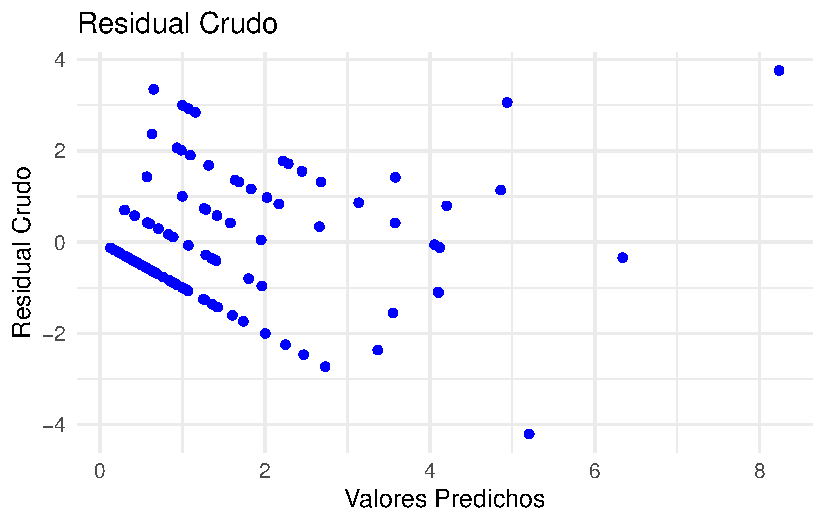
\includegraphics{Modelos_files/figure-pdf/unnamed-chunk-37-1.pdf}\end{minipage}%
%
\begin{minipage}{0.50\linewidth}
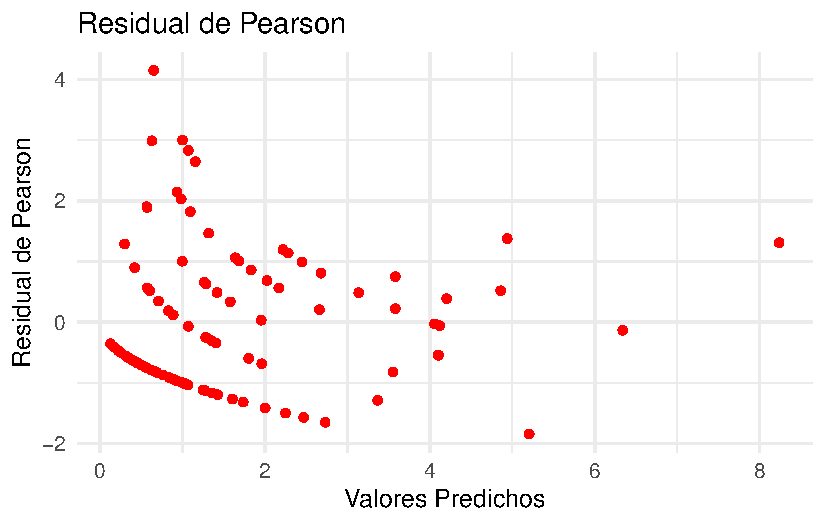
\includegraphics{Modelos_files/figure-pdf/unnamed-chunk-37-2.pdf}\end{minipage}%
\newline
\begin{minipage}{0.50\linewidth}
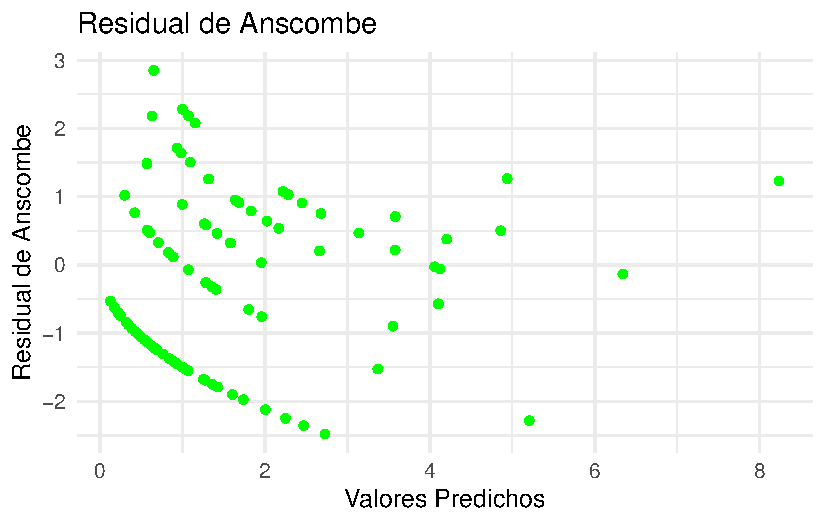
\includegraphics{Modelos_files/figure-pdf/unnamed-chunk-37-3.pdf}\end{minipage}%
%
\begin{minipage}{0.50\linewidth}
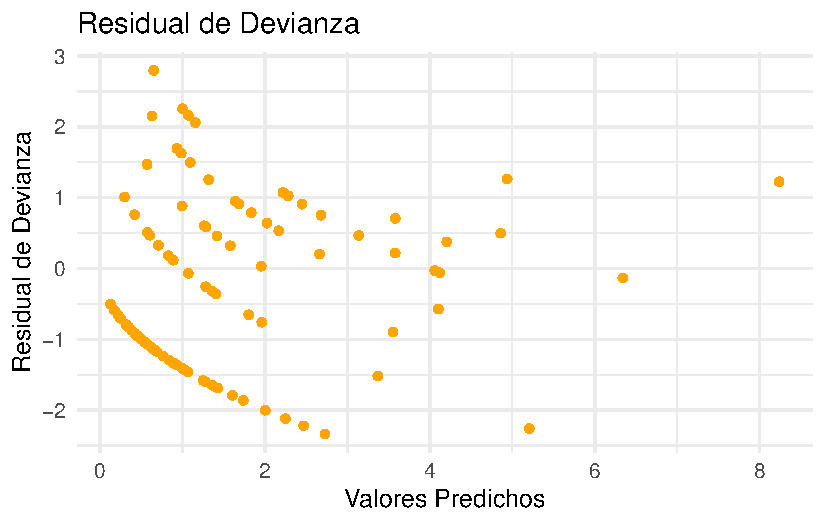
\includegraphics{Modelos_files/figure-pdf/unnamed-chunk-37-4.pdf}\end{minipage}%

\end{figure}%

Aún con las interacciones el modelo no parece ser adecuado.

\subsection{Regresión Binomial}\label{regresiuxf3n-binomial}

\section{Residuales}\label{residuales-1}

\begin{itemize}
\tightlist
\item
  \textbf{Residuales crudos (o de respuesta):} \[y-\hat{\mu}\]
  -\textbf{Residuales de Pearson:}
  \[r_{P}=\frac{y-n\hat{\pi}}{\sqrt{n\hat{\pi}(1-\hat{\pi})}}\]
\end{itemize}

-\textbf{Residuales de desviación:} \[r_{D}=sign(y-\mu)\sqrt{d_{i}},\]
Para el caso de la Poisson:
\[r_{D}=sign(y-\mu)\sqrt{2()ylog(\frac{y}{\mu})-y+\mu}\]

-\textbf{Residuales de Anscombe:}
\[A(.)=\int\frac{d\mu}{\mu^{1/3}}=\frac{3}{2}\mu^{2/3}=\frac{3}{2}(n\pi)^{2/3}\]
Para la distribución Binomial:
\[r_{A}=\frac{A(y)-A(\mu)}{\sqrt{V(A(y))}}\approx\frac{A(y)-A(\mu)}{\sqrt{(A'(\mu))^{2}V(\mu)}}\Longrightarrow\frac{\frac{3}{2}((\frac{y}{n})^{2/3}-\pi^{2/3})}{(\frac{\pi(1-\pi)}{n})^{1/6}}\]
- Sean \(Y_1, Y_2, \cdots, Y_n\) variables aleatorias independientes con
distribución \emph{Binomial}, tales que

\begin{verbatim}
$$Y_i \sim Binomial(n_i, p_i) \quad i=1,2,\cdots,n.$$
donde $n_i$ es el número de ensayos (conocido) para la observación $i$, y $p_i$ es la probabilidad de éxito. La variable $Y_i$ representa el número de éxitos en los $n_i$ ensayos.
\end{verbatim}

\begin{itemize}
\item
  La media de \(Y_i\) es \(\mu_i = E[Y_i] = n_i p_i\).
\item
  La función de enlace canónica (y más común) para la probabilidad
  \(p_i\) es la \textbf{logit}:

  \[\eta_i = logit(p_i) = \ln\left(\frac{p_i}{1-p_i}\right)\] donde
  \(\eta_i\) es el predictor lineal:
  \[\eta_i = \beta_0 + \beta_1X_{i1} + \beta_2X_{i2} + \cdots + \beta_pX_{ip} = x_i^T \beta\]
\item
  La relación inversa, que expresa la probabilidad \(p_i\) en función
  del predictor lineal, es la \textbf{función logística}:
  \[p_i = \frac{e^{\eta_i}}{1+e^{\eta_i}}\] Y por lo tanto, la media
  \(\mu_i\) se relaciona con \(\eta_i\) a través de:
  \[\mu_i = n_i p_i = n_i \frac{e^{\eta_i}}{1+e^{\eta_i}}\]
\item
  La función de log-verosimilitud (ignorando términos constantes como
  \(\ln\binom{n_i}{y_i}\)) es: \[
  \begin{align*}
  \mathcal{l}(\beta) &= \sum_{i=1}^n \left[y_i\ln(p_i) + (n_i - y_i)\ln(1-p_i)\right]\\
  &= \sum_{i=1}^n \left[y_i \eta_i - n_i \ln(1+e^{\eta_i})\right] \\
  &= \sum_{i=1}^n \left[y_i (x_i^T \beta) - n_i \ln(1+\exp(x_i^T \beta))\right]
  \end{align*}
  \]
\item
  La \textbf{función score} (vector de primeras derivadas) se puede
  derivar y resulta ser:
  \[\frac{\partial \mathcal{l}(\beta)}{\partial \beta} = \sum_{i=1}^n (y_i - n_i p_i)x_i = \sum_{i=1}^n (y_i - \mu_i)x_i = X^t(y - \mu)\]
\item
  La \textbf{Matriz de Información de Fisher} es \(I(\beta) = X^tWX\),
  donde \(W\) es una matriz diagonal. Para calcular los elementos
  \(w_{ii}\) de \(W\), necesitamos la varianza \(Var(Y_i)\) y la
  derivada \(d\mu_i / d\eta_i\): \[Var(Y_i) = n_i p_i (1-p_i)\]
  \[\frac{\partial \mu_i}{\partial \eta_i} = \frac{\partial (n_i p_i)}{\partial \eta_i} = n_i \frac{\partial p_i}{\partial \eta_i} = n_i \frac{e^{\eta_i}}{(1+e^{\eta_i})^2} = n_i p_i (1-p_i)\]
  Entonces, los pesos son:
  \[w_{ii} = \frac{\left(\frac{\partial \mu_i}{\partial \eta_i}\right)^2}{Var(y_i)} = \frac{(n_i p_i (1-p_i))^2}{n_i p_i (1-p_i)} = n_i p_i (1-p_i)\]
\item
  Nuestro \(\widetilde{y}\) para el algoritmo Fisher Scoring es:
  \[\widetilde{y} = \eta_i + (y_i - \mu_i)\frac{\partial \eta_i}{\partial \mu_i}\]
  Dado que
  \(\frac{\partial \eta_i}{\partial \mu_i} = \left(\frac{\partial \mu_i}{\partial \eta_i}\right)^{-1} = \frac{1}{n_i p_i (1-p_i)}\),
  tenemos:
  \[\widetilde{y} = \eta_i + \frac{y_i - \mu_i}{n_i p_i (1-p_i)}\]
\item
  El \textbf{Algoritmo de Fisher-Scoring} para la regresión binomial
  (logit) es:

  \begin{enumerate}
  \def\labelenumi{\arabic{enumi}.}
  \tightlist
  \item
    Iniciar con un valor \(\beta^{(0)}\).
  \item
    Obtener \(\beta^{(k+1)}\) a partir de \(\beta^{(k)}\) usando:

    \begin{enumerate}
    \def\labelenumii{\alph{enumii}.}
    \tightlist
    \item
      Calcular \(\eta^{(k)} = X \beta^{(k)}\).
    \item
      Calcular \(p^{(k)}_i = 1 / (1 + \exp(-\eta^{(k)}_i))\).
    \item
      Calcular \(\mu^{(k)}_i = n_i p^{(k)}_i\).
    \item
      Calcular pesos \(w^{(k)}_{ii} = n_i p^{(k)}_i (1-p^{(k)}_i)\).
      Formar \(W^{(k)}\).
    \item
      Calcular
      \(\widetilde{y}^{(k)}_i = \eta^{(k)}_i + (y_i - \mu^{(k)}_i) / w^{(k)}_{ii}\).
      Formar \(\widetilde{y}^{(k)}\).
    \item
      Actualizar
      \(\beta^{(k+1)} = \left(X^tW^{(k)}X\right)^{-1}X^tW^{(k)}\widetilde{y}^{(k)}\).
    \end{enumerate}
  \item
    Repetir el paso (2) hasta la convergencia.
  \end{enumerate}
\end{itemize}

\subsubsection{Datos simulados}\label{datos-simulados}

A continuación, adaptaremos el algoritmo para un caso binomial usando
datos generados por simulación.

\begin{Shaded}
\begin{Highlighting}[]
\DocumentationTok{\#\# Población binomial}
\CommentTok{\# Parámetros}
\FunctionTok{set.seed}\NormalTok{(}\DecValTok{1040}\NormalTok{)}
\NormalTok{n }\OtherTok{\textless{}{-}} \DecValTok{100}
\NormalTok{beta }\OtherTok{\textless{}{-}} \FunctionTok{c}\NormalTok{(}\DecValTok{0}\NormalTok{, }\FloatTok{0.2}\NormalTok{)}
\end{Highlighting}
\end{Shaded}

\begin{Shaded}
\begin{Highlighting}[]
\CommentTok{\# Simulación de datos}
\NormalTok{xbin }\OtherTok{\textless{}{-}} \FunctionTok{runif}\NormalTok{(n, }\AttributeTok{min =} \DecValTok{0}\NormalTok{, }\AttributeTok{max =} \DecValTok{10}\NormalTok{)}
\NormalTok{X2 }\OtherTok{\textless{}{-}} \FunctionTok{model.matrix}\NormalTok{(}\SpecialCharTok{\textasciitilde{}}\NormalTok{ xbin)  }\CommentTok{\# Incluye intercepto automáticamente}
\NormalTok{eta }\OtherTok{\textless{}{-}}\NormalTok{ X2 }\SpecialCharTok{\%*\%}\NormalTok{ beta}
\end{Highlighting}
\end{Shaded}

\begin{Shaded}
\begin{Highlighting}[]
\CommentTok{\# Dataset simulado}
\NormalTok{pi }\OtherTok{\textless{}{-}} \FunctionTok{exp}\NormalTok{(eta)}\SpecialCharTok{/}\NormalTok{(}\DecValTok{1}\SpecialCharTok{+}\FunctionTok{exp}\NormalTok{(eta))}
\NormalTok{yb }\OtherTok{\textless{}{-}} \FunctionTok{c}\NormalTok{()}
\ControlFlowTok{for}\NormalTok{ (i }\ControlFlowTok{in} \DecValTok{1}\SpecialCharTok{:}\NormalTok{n) \{}
\NormalTok{  yb[i] }\OtherTok{\textless{}{-}} \FunctionTok{rbinom}\NormalTok{(}\DecValTok{1}\NormalTok{,}\AttributeTok{size =} \DecValTok{1}\NormalTok{,}\AttributeTok{prob =}\NormalTok{ pi[i])}
\NormalTok{\}}

\NormalTok{data\_bin }\OtherTok{\textless{}{-}} \FunctionTok{tibble}\NormalTok{(}\AttributeTok{y =}\NormalTok{ yb, }\AttributeTok{x =}\NormalTok{ xbin)}
\end{Highlighting}
\end{Shaded}

A continuación se presentan los datos simulados

\begin{Shaded}
\begin{Highlighting}[]
\FunctionTok{ggplot}\NormalTok{(data\_bin, }\FunctionTok{aes}\NormalTok{(}\AttributeTok{x =}\NormalTok{ x, }\AttributeTok{y =}\NormalTok{ y)) }\SpecialCharTok{+}
    \FunctionTok{geom\_jitter}\NormalTok{(}\AttributeTok{height =} \FloatTok{0.02}\NormalTok{, }\AttributeTok{width =} \DecValTok{0}\NormalTok{, }
                \AttributeTok{alpha =} \FloatTok{0.6}\NormalTok{, }\AttributeTok{size =} \DecValTok{3}\NormalTok{, }\AttributeTok{color =} \StringTok{"\#1f77b4"}\NormalTok{) }\SpecialCharTok{+}
  \FunctionTok{ggtitle}\NormalTok{(}\StringTok{"Distribución binomial {-} Datos simulados"}\NormalTok{) }\SpecialCharTok{+}
  \FunctionTok{theme\_minimal}\NormalTok{(}\DecValTok{12}\NormalTok{)}
\end{Highlighting}
\end{Shaded}

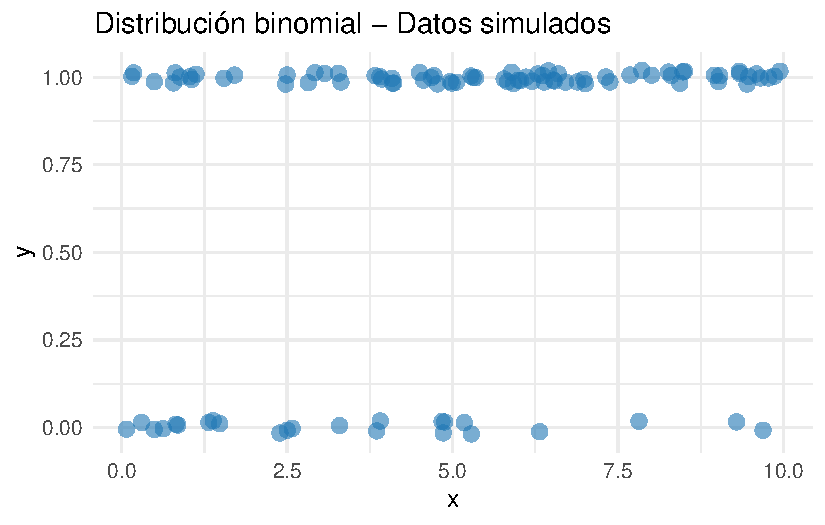
\includegraphics[width=1\textwidth,height=\textheight]{Modelos_files/figure-pdf/unnamed-chunk-41-1.pdf}

\subsubsection{Algoritmo de
Fisher-Scoring}\label{algoritmo-de-fisher-scoring-1}

El algoritmo de Fisher-Scoring para la regresión logística se presenta a
continuación

\begin{Shaded}
\begin{Highlighting}[]
\CommentTok{\# Creación de la función}
\NormalTok{fisher\_scoring\_binomial }\OtherTok{\textless{}{-}} \ControlFlowTok{function}\NormalTok{(y, X, beta\_init, }\AttributeTok{tol =} \FloatTok{1e{-}5}\NormalTok{, }\AttributeTok{max\_iter =} \DecValTok{100}\NormalTok{) \{}
\NormalTok{  beta }\OtherTok{\textless{}{-}}\NormalTok{ beta\_init}
  \ControlFlowTok{for}\NormalTok{ (iter }\ControlFlowTok{in} \DecValTok{1}\SpecialCharTok{:}\NormalTok{max\_iter) \{}
\NormalTok{    eta }\OtherTok{\textless{}{-}}\NormalTok{ X }\SpecialCharTok{\%*\%}\NormalTok{ beta}
    
\NormalTok{    pi }\OtherTok{\textless{}{-}} \FunctionTok{exp}\NormalTok{(eta) }\SpecialCharTok{/}\NormalTok{ (}\DecValTok{1} \SpecialCharTok{+} \FunctionTok{exp}\NormalTok{(eta))}
\NormalTok{    pi }\OtherTok{\textless{}{-}} \FunctionTok{pmax}\NormalTok{(}\FunctionTok{pmin}\NormalTok{(pi, }\DecValTok{1} \SpecialCharTok{{-}} \FloatTok{1e{-}10}\NormalTok{), }\FloatTok{1e{-}10}\NormalTok{)}
    
\NormalTok{    W }\OtherTok{\textless{}{-}} \FunctionTok{diag}\NormalTok{(}\FunctionTok{as.vector}\NormalTok{(pi }\SpecialCharTok{*}\NormalTok{ (}\DecValTok{1} \SpecialCharTok{{-}}\NormalTok{ pi)))}
    
\NormalTok{    z }\OtherTok{\textless{}{-}}\NormalTok{ eta }\SpecialCharTok{+}\NormalTok{ (y }\SpecialCharTok{{-}}\NormalTok{ pi) }\SpecialCharTok{/}\NormalTok{ (pi }\SpecialCharTok{*}\NormalTok{ (}\DecValTok{1} \SpecialCharTok{{-}}\NormalTok{ pi))}
    
\NormalTok{    beta\_new }\OtherTok{\textless{}{-}} \FunctionTok{tryCatch}\NormalTok{(\{}
      \FunctionTok{solve}\NormalTok{(}\FunctionTok{t}\NormalTok{(X) }\SpecialCharTok{\%*\%}\NormalTok{ W }\SpecialCharTok{\%*\%}\NormalTok{ X) }\SpecialCharTok{\%*\%}\NormalTok{ (}\FunctionTok{t}\NormalTok{(X) }\SpecialCharTok{\%*\%}\NormalTok{ W }\SpecialCharTok{\%*\%}\NormalTok{ z)}
\NormalTok{    \}, }\AttributeTok{error =} \ControlFlowTok{function}\NormalTok{(e) \{}
      \FunctionTok{stop}\NormalTok{(}\StringTok{"Fallo al invertir la matriz. ¿X tiene multicolinealidad?"}\NormalTok{)}
\NormalTok{    \})}
    
    \CommentTok{\# guardamos la matriz de varianzas y covarianzas de los betas}
\NormalTok{    cov\_beta }\OtherTok{\textless{}{-}} \FunctionTok{solve}\NormalTok{(}\FunctionTok{t}\NormalTok{(X) }\SpecialCharTok{\%*\%}\NormalTok{ W }\SpecialCharTok{\%*\%}\NormalTok{ X)}
    
    \ControlFlowTok{if}\NormalTok{ (}\FunctionTok{max}\NormalTok{(}\FunctionTok{abs}\NormalTok{(beta\_new }\SpecialCharTok{{-}}\NormalTok{ beta), }\AttributeTok{na.rm =} \ConstantTok{TRUE}\NormalTok{) }\SpecialCharTok{\textless{}}\NormalTok{ tol) \{}
      \FunctionTok{message}\NormalTok{(}\StringTok{"Convergió en iteración "}\NormalTok{, iter)}
\NormalTok{      pi\_hat }\OtherTok{\textless{}{-}} \FunctionTok{exp}\NormalTok{(X }\SpecialCharTok{\%*\%}\NormalTok{ beta\_new) }\SpecialCharTok{/}\NormalTok{ (}\DecValTok{1} \SpecialCharTok{+} \FunctionTok{exp}\NormalTok{(X }\SpecialCharTok{\%*\%}\NormalTok{ beta\_new))}
\NormalTok{      pi\_hat }\OtherTok{\textless{}{-}} \FunctionTok{pmax}\NormalTok{(}\FunctionTok{pmin}\NormalTok{(pi\_hat, }\DecValTok{1} \SpecialCharTok{{-}} \FloatTok{1e{-}10}\NormalTok{), }\FloatTok{1e{-}10}\NormalTok{) }
      \CommentTok{\# Resdiaul crudo}
\NormalTok{      residual }\OtherTok{\textless{}{-}}\NormalTok{ y}\SpecialCharTok{{-}}\NormalTok{pi\_hat}
      \CommentTok{\# Residual de pearson}
\NormalTok{      residual\_pearson }\OtherTok{\textless{}{-}}\NormalTok{ (y }\SpecialCharTok{{-}}\NormalTok{ pi\_hat) }\SpecialCharTok{/} \FunctionTok{sqrt}\NormalTok{(pi\_hat)}
      \CommentTok{\# Residual de Anscombe}
\NormalTok{      residual\_anscombe }\OtherTok{\textless{}{-}}\NormalTok{ (}\DecValTok{3}\SpecialCharTok{/}\DecValTok{2}\NormalTok{)}\SpecialCharTok{*}\NormalTok{(y}\SpecialCharTok{\^{}}\NormalTok{(}\DecValTok{2}\SpecialCharTok{/}\DecValTok{3}\NormalTok{)}\SpecialCharTok{{-}}\NormalTok{pi\_hat}\SpecialCharTok{\^{}}\NormalTok{(}\DecValTok{2}\SpecialCharTok{/}\DecValTok{3}\NormalTok{))}\SpecialCharTok{/}\NormalTok{((pi\_hat}\SpecialCharTok{*}\NormalTok{(}\DecValTok{1}\SpecialCharTok{{-}}\NormalTok{pi\_hat))}\SpecialCharTok{\^{}}\NormalTok{(}\DecValTok{1}\SpecialCharTok{/}\DecValTok{3}\NormalTok{))}
      \CommentTok{\# Residual de devianza}
      \CommentTok{\# Handle y=0 and y=1 cases for deviance}
\NormalTok{      dev }\OtherTok{\textless{}{-}} \FunctionTok{ifelse}\NormalTok{(y }\SpecialCharTok{==} \DecValTok{0}\NormalTok{, }\DecValTok{2} \SpecialCharTok{*}\NormalTok{ pi\_hat, }\FunctionTok{ifelse}\NormalTok{(y }\SpecialCharTok{==} \DecValTok{1}\NormalTok{, }\DecValTok{2} \SpecialCharTok{*}\NormalTok{ (}\DecValTok{1} \SpecialCharTok{{-}}\NormalTok{ pi\_hat),}
                    \FunctionTok{sqrt}\NormalTok{(}\DecValTok{2} \SpecialCharTok{*}\NormalTok{ (y }\SpecialCharTok{*} \FunctionTok{log}\NormalTok{(y }\SpecialCharTok{/}\NormalTok{ pi\_hat) }\SpecialCharTok{+}\NormalTok{ (}\DecValTok{1} \SpecialCharTok{{-}}\NormalTok{ y) }\SpecialCharTok{*} \FunctionTok{log}\NormalTok{((}\DecValTok{1} \SpecialCharTok{{-}}\NormalTok{ y) }\SpecialCharTok{/}\NormalTok{ (}\DecValTok{1} \SpecialCharTok{{-}}\NormalTok{ pi\_hat))))))}
\NormalTok{      residual\_deviance }\OtherTok{\textless{}{-}} \FunctionTok{sign}\NormalTok{(y }\SpecialCharTok{{-}}\NormalTok{ pi\_hat) }\SpecialCharTok{*} \FunctionTok{sqrt}\NormalTok{(dev)}
      \FunctionTok{return}\NormalTok{(}\FunctionTok{list}\NormalTok{(}\AttributeTok{beta =} \FunctionTok{as.vector}\NormalTok{(beta\_new), }\AttributeTok{predichos =}\NormalTok{ pi\_hat,}
                  \AttributeTok{covarianza =}\NormalTok{ cov\_beta,}
                  \AttributeTok{residual =}\NormalTok{ residual,}
                  \AttributeTok{residual\_pearson =}\NormalTok{ residual\_pearson,}
                  \AttributeTok{residual\_anscombe =}\NormalTok{ residual\_anscombe,}
                  \AttributeTok{residual\_deviance =}\NormalTok{ residual\_deviance))}
\NormalTok{    \}}
    
\NormalTok{    beta }\OtherTok{\textless{}{-}}\NormalTok{ beta\_new}
\NormalTok{  \}}
  \FunctionTok{warning}\NormalTok{(}\StringTok{"No convergió"}\NormalTok{)}
  \FunctionTok{return}\NormalTok{(}\FunctionTok{as.vector}\NormalTok{(beta))}
\NormalTok{\}}
\end{Highlighting}
\end{Shaded}

\begin{Shaded}
\begin{Highlighting}[]
\CommentTok{\# Ejecutamos la función}

\NormalTok{beta\_binomial }\OtherTok{\textless{}{-}} \FunctionTok{fisher\_scoring\_binomial}\NormalTok{(}\AttributeTok{y =}\NormalTok{ yb, }\AttributeTok{X =}\NormalTok{ X2, }
                                         \AttributeTok{beta\_init =} \FunctionTok{rep}\NormalTok{(}\FloatTok{0.01}\NormalTok{, }\FunctionTok{ncol}\NormalTok{(X2)))}
\end{Highlighting}
\end{Shaded}

\begin{verbatim}
Convergió en iteración 5
\end{verbatim}

\begin{Shaded}
\begin{Highlighting}[]
\CommentTok{\# Estimación de los parámetros del modelo}

\FunctionTok{names}\NormalTok{(beta\_binomial}\SpecialCharTok{$}\NormalTok{beta) }\OtherTok{\textless{}{-}} \FunctionTok{colnames}\NormalTok{(X2)}
\NormalTok{beta\_binomial}\SpecialCharTok{$}\NormalTok{beta}
\end{Highlighting}
\end{Shaded}

\begin{verbatim}
(Intercept)        xbin 
-0.05789329  0.26830824 
\end{verbatim}

\begin{Shaded}
\begin{Highlighting}[]
\NormalTok{modelo\_logistico }\OtherTok{\textless{}{-}} \FunctionTok{glm}\NormalTok{(yb }\SpecialCharTok{\textasciitilde{}}\NormalTok{ X2 }\SpecialCharTok{{-}} \DecValTok{1}\NormalTok{, }\AttributeTok{family =} \FunctionTok{binomial}\NormalTok{(}\AttributeTok{link =} \StringTok{"logit"}\NormalTok{))}

\NormalTok{modelo\_logistico}\SpecialCharTok{$}\NormalTok{coefficients}
\end{Highlighting}
\end{Shaded}

\begin{verbatim}
X2(Intercept)        X2xbin 
  -0.05789329    0.26830824 
\end{verbatim}

\begin{longtable}[]{@{}
  >{\raggedright\arraybackslash}p{(\columnwidth - 4\tabcolsep) * \real{0.2500}}
  >{\centering\arraybackslash}p{(\columnwidth - 4\tabcolsep) * \real{0.4286}}
  >{\centering\arraybackslash}p{(\columnwidth - 4\tabcolsep) * \real{0.3214}}@{}}
\toprule\noalign{}
\begin{minipage}[b]{\linewidth}\raggedright
Variable
\end{minipage} & \begin{minipage}[b]{\linewidth}\centering
fisher\_scoring\_binomial
\end{minipage} & \begin{minipage}[b]{\linewidth}\centering
glm
\end{minipage} \\
\midrule\noalign{}
\endhead
\bottomrule\noalign{}
\endlastfoot
(Intercept) & \(\hat{\beta_0} = -0.05789329\) &
\(\hat{\beta_0} = -0.05789329\) \\
xbin & \(\hat{\beta_1} = 0.26830824\) &
\(\hat{\beta_1} = 0.26830824\) \\
\end{longtable}

La matriz de covarianza estimada obtenida mediante el algoritmo de
Fisher-Scoring coincide con la obtenida a través de la función
\texttt{glm}, salvo por algunas diferencias numéricas muy pequeñas

\begin{Shaded}
\begin{Highlighting}[]
\NormalTok{beta\_binomial}\SpecialCharTok{$}\NormalTok{covarianza; }\FunctionTok{vcov}\NormalTok{(modelo\_logistico)}
\end{Highlighting}
\end{Shaded}

\begin{verbatim}
            (Intercept)         xbin
(Intercept)  0.19628250 -0.033856568
xbin        -0.03385657  0.008452617
\end{verbatim}

\begin{verbatim}
              X2(Intercept)      X2xbin
X2(Intercept)    0.19628179 -0.03385631
X2xbin          -0.03385631  0.00845250
\end{verbatim}

La matriz de covarianza es prácticamente la misma con ambos métodos.

\subsubsection{Residuales}\label{residuales-2}

A continuación, se muestran gráficamente los cuatro tipos de residuales
calculados: \emph{residuales crudos}, \emph{residuales de pearson},
\emph{residuales de Anscombe} y \emph{residuales de devianza}

\begin{Shaded}
\begin{Highlighting}[]
\NormalTok{df\_residuals }\OtherTok{\textless{}{-}} \FunctionTok{data.frame}\NormalTok{(}
    \AttributeTok{predichos =}\NormalTok{ beta\_binomial}\SpecialCharTok{$}\NormalTok{predichos,}
    \AttributeTok{residual =}\NormalTok{ beta\_binomial}\SpecialCharTok{$}\NormalTok{residual,}
    \AttributeTok{residual\_pearson =}\NormalTok{ beta\_binomial}\SpecialCharTok{$}\NormalTok{residual\_pearson,}
    \AttributeTok{residual\_anscombe =}\NormalTok{ beta\_binomial}\SpecialCharTok{$}\NormalTok{residual\_anscombe,}
    \AttributeTok{residual\_deviance =}\NormalTok{ beta\_binomial}\SpecialCharTok{$}\NormalTok{residual\_deviance}
\NormalTok{  )}
\end{Highlighting}
\end{Shaded}

\begin{Shaded}
\begin{Highlighting}[]
\CommentTok{\# Gráfico de los tres tipos de residuales}

\NormalTok{p1 }\OtherTok{\textless{}{-}} \FunctionTok{ggplot}\NormalTok{(df\_residuals, }\FunctionTok{aes}\NormalTok{(}\AttributeTok{x =}\NormalTok{ predichos, }\AttributeTok{y =}\NormalTok{ residual)) }\SpecialCharTok{+}
    \FunctionTok{geom\_point}\NormalTok{(}\AttributeTok{color =} \StringTok{\textquotesingle{}blue\textquotesingle{}}\NormalTok{) }\SpecialCharTok{+}
    \FunctionTok{labs}\NormalTok{(}\AttributeTok{title =} \StringTok{\textquotesingle{}Residual Crudo\textquotesingle{}}\NormalTok{, }\AttributeTok{x =} \StringTok{\textquotesingle{}Valores Predichos\textquotesingle{}}\NormalTok{, }\AttributeTok{y =} \StringTok{\textquotesingle{}Residual Crudo\textquotesingle{}}\NormalTok{) }\SpecialCharTok{+}
    \FunctionTok{theme\_minimal}\NormalTok{(}\DecValTok{12}\NormalTok{)}

\NormalTok{p2 }\OtherTok{\textless{}{-}} \FunctionTok{ggplot}\NormalTok{(df\_residuals, }\FunctionTok{aes}\NormalTok{(}\AttributeTok{x =}\NormalTok{ predichos, }\AttributeTok{y =}\NormalTok{ residual\_pearson)) }\SpecialCharTok{+}
    \FunctionTok{geom\_point}\NormalTok{(}\AttributeTok{color =} \StringTok{\textquotesingle{}red\textquotesingle{}}\NormalTok{) }\SpecialCharTok{+}
    \FunctionTok{labs}\NormalTok{(}\AttributeTok{title =} \StringTok{\textquotesingle{}Residual de Pearson\textquotesingle{}}\NormalTok{, }\AttributeTok{x =} \StringTok{\textquotesingle{}Valores Predichos\textquotesingle{}}\NormalTok{, }\AttributeTok{y =} \StringTok{\textquotesingle{}Residual de Pearson\textquotesingle{}}\NormalTok{) }\SpecialCharTok{+}
    \FunctionTok{theme\_minimal}\NormalTok{(}\DecValTok{12}\NormalTok{)}

\NormalTok{p3 }\OtherTok{\textless{}{-}} \FunctionTok{ggplot}\NormalTok{(df\_residuals, }\FunctionTok{aes}\NormalTok{(}\AttributeTok{x =}\NormalTok{ predichos, }\AttributeTok{y =}\NormalTok{ residual\_anscombe)) }\SpecialCharTok{+}
    \FunctionTok{geom\_point}\NormalTok{(}\AttributeTok{color =} \StringTok{\textquotesingle{}green\textquotesingle{}}\NormalTok{) }\SpecialCharTok{+}
    \FunctionTok{labs}\NormalTok{(}\AttributeTok{title =} \StringTok{\textquotesingle{}Residual de Anscombe\textquotesingle{}}\NormalTok{, }\AttributeTok{x =} \StringTok{\textquotesingle{}Valores Predichos\textquotesingle{}}\NormalTok{, }\AttributeTok{y =} \StringTok{\textquotesingle{}Residual de Anscombe\textquotesingle{}}\NormalTok{) }\SpecialCharTok{+}
    \FunctionTok{theme\_minimal}\NormalTok{(}\DecValTok{12}\NormalTok{)}

\NormalTok{p4 }\OtherTok{\textless{}{-}} \FunctionTok{ggplot}\NormalTok{(df\_residuals, }\FunctionTok{aes}\NormalTok{(}\AttributeTok{x =}\NormalTok{ predichos, }\AttributeTok{y =}\NormalTok{ residual\_deviance)) }\SpecialCharTok{+}
    \FunctionTok{geom\_point}\NormalTok{(}\AttributeTok{color =} \StringTok{\textquotesingle{}orange\textquotesingle{}}\NormalTok{) }\SpecialCharTok{+}
    \FunctionTok{labs}\NormalTok{(}\AttributeTok{title =} \StringTok{\textquotesingle{}Residual de Devianza\textquotesingle{}}\NormalTok{, }\AttributeTok{x =} \StringTok{\textquotesingle{}Valores Predichos\textquotesingle{}}\NormalTok{, }\AttributeTok{y =} \StringTok{\textquotesingle{}Residual de Devianza\textquotesingle{}}\NormalTok{) }\SpecialCharTok{+}
    \FunctionTok{theme\_minimal}\NormalTok{(}\DecValTok{12}\NormalTok{)}
\end{Highlighting}
\end{Shaded}

\begin{Shaded}
\begin{Highlighting}[]
\NormalTok{p1; p2; p3; p4}
\end{Highlighting}
\end{Shaded}

\begin{figure}

\begin{minipage}{0.50\linewidth}
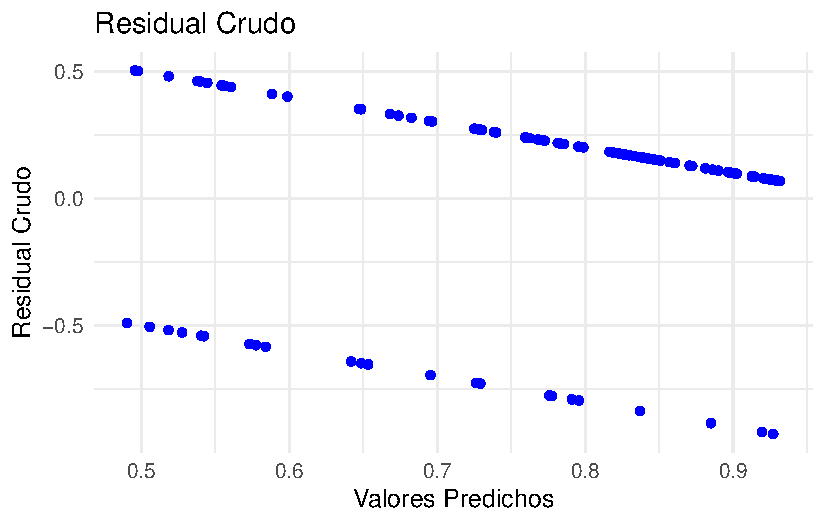
\includegraphics{Modelos_files/figure-pdf/unnamed-chunk-48-1.pdf}\end{minipage}%
%
\begin{minipage}{0.50\linewidth}
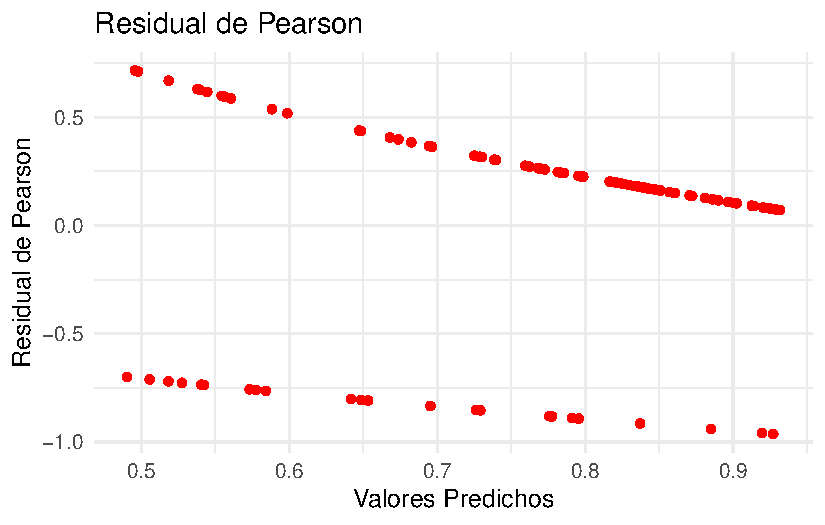
\includegraphics{Modelos_files/figure-pdf/unnamed-chunk-48-2.pdf}\end{minipage}%
\newline
\begin{minipage}{0.50\linewidth}
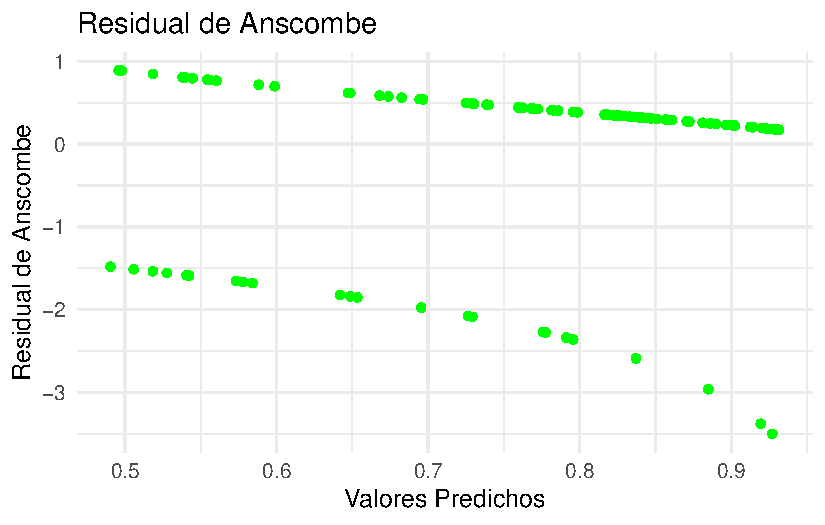
\includegraphics{Modelos_files/figure-pdf/unnamed-chunk-48-3.pdf}\end{minipage}%
%
\begin{minipage}{0.50\linewidth}
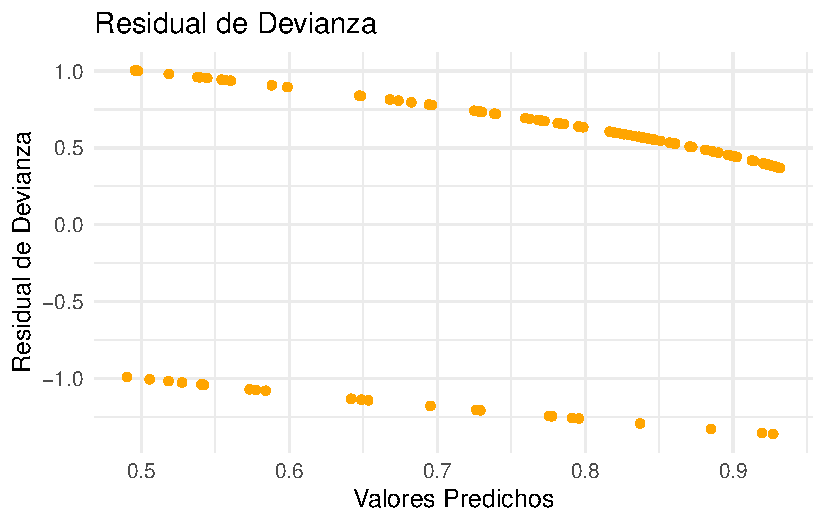
\includegraphics{Modelos_files/figure-pdf/unnamed-chunk-48-4.pdf}\end{minipage}%

\end{figure}%

\subsubsection{Regresión logística con los datos del
agua}\label{regresiuxf3n-loguxedstica-con-los-datos-del-agua}

A continuación, se utilizarán datos relacionados con tratamientos
aplicados al agua. La variable de respuesta indica si se utilizó o no un
polímero.

\begin{Shaded}
\begin{Highlighting}[]
\NormalTok{TURB}\OtherTok{=}\FunctionTok{c}\NormalTok{(}\DecValTok{300}\NormalTok{,}\DecValTok{250}\NormalTok{,}\DecValTok{190}\NormalTok{,}\DecValTok{160}\NormalTok{,}\DecValTok{560}\NormalTok{,}\DecValTok{150}\NormalTok{,}\DecValTok{160}\NormalTok{,}\DecValTok{270}\NormalTok{,}\DecValTok{450}\NormalTok{,}\DecValTok{210}\NormalTok{,}\DecValTok{420}\NormalTok{,}\DecValTok{550}\NormalTok{,}\DecValTok{1200}\NormalTok{,}\DecValTok{420}\NormalTok{,}\DecValTok{500}\NormalTok{,}\DecValTok{150}\NormalTok{,}\DecValTok{200}\NormalTok{,}\DecValTok{390}\NormalTok{,}\DecValTok{380}\NormalTok{,}\DecValTok{140}\NormalTok{,}\DecValTok{170}\NormalTok{,}\DecValTok{1110}\NormalTok{,}\DecValTok{140}\NormalTok{,}\DecValTok{150}\NormalTok{,}\DecValTok{870}\NormalTok{,}\DecValTok{720}\NormalTok{,}\DecValTok{430}\NormalTok{,}\DecValTok{550}\NormalTok{)}

\NormalTok{COL}\OtherTok{=}\FunctionTok{c}\NormalTok{(}\DecValTok{100}\NormalTok{,}\DecValTok{100}\NormalTok{,}\DecValTok{50}\NormalTok{,}\DecValTok{70}\NormalTok{,}\DecValTok{200}\NormalTok{,}\DecValTok{100}\NormalTok{,}\DecValTok{100}\NormalTok{,}\DecValTok{70}\NormalTok{,}\DecValTok{130}\NormalTok{,}\DecValTok{100}\NormalTok{,}\DecValTok{100}\NormalTok{,}\DecValTok{250}\NormalTok{,}\DecValTok{250}\NormalTok{,}\DecValTok{100}\NormalTok{,}\DecValTok{120}\NormalTok{,}\DecValTok{75}\NormalTok{,}\DecValTok{50}\NormalTok{,}\DecValTok{140}\NormalTok{,}\DecValTok{120}\NormalTok{,}\DecValTok{50}\NormalTok{,}\DecValTok{110}\NormalTok{,}\DecValTok{100}\NormalTok{,}\DecValTok{80}\NormalTok{,}\DecValTok{90}\NormalTok{,}\DecValTok{150}\NormalTok{,}\DecValTok{200}\NormalTok{,}\DecValTok{100}\NormalTok{,}\DecValTok{200}\NormalTok{)}

\NormalTok{ALCA}\OtherTok{=}\FunctionTok{c}\NormalTok{(}\DecValTok{49}\NormalTok{,}\DecValTok{43}\NormalTok{,}\DecValTok{51}\NormalTok{,}\DecValTok{52}\NormalTok{,}\DecValTok{44}\NormalTok{,}\DecValTok{48}\NormalTok{,}\DecValTok{55}\NormalTok{,}\DecValTok{43}\NormalTok{,}\DecValTok{56}\NormalTok{,}\DecValTok{51}\NormalTok{,}\DecValTok{46}\NormalTok{,}\DecValTok{65}\NormalTok{,}\DecValTok{43}\NormalTok{,}\DecValTok{53}\NormalTok{,}\DecValTok{48}\NormalTok{,}\DecValTok{45}\NormalTok{,}\DecValTok{52}\NormalTok{,}\DecValTok{52}\NormalTok{,}\DecValTok{39}\NormalTok{,}\DecValTok{54}\NormalTok{,}\DecValTok{52}\NormalTok{,}\DecValTok{51}\NormalTok{,}\DecValTok{55}\NormalTok{,}\DecValTok{50}\NormalTok{,}\DecValTok{49}\NormalTok{,}\DecValTok{44}\NormalTok{,}\DecValTok{48}\NormalTok{,}\DecValTok{40}\NormalTok{)}

\NormalTok{PH}\OtherTok{=}\FunctionTok{c}\NormalTok{(}\FloatTok{8.33}\NormalTok{,}\FloatTok{7.64}\NormalTok{,}\FloatTok{7.62}\NormalTok{,}\FloatTok{7.62}\NormalTok{,}\FloatTok{8.19}\NormalTok{,}\FloatTok{7.90}\NormalTok{,}\FloatTok{7.60}\NormalTok{,}\FloatTok{8.07}\NormalTok{,}\FloatTok{7.53}\NormalTok{,}\FloatTok{7.72}\NormalTok{,}\FloatTok{7.90}\NormalTok{,}\FloatTok{7.68}\NormalTok{,}\FloatTok{7.93}\NormalTok{,}\FloatTok{7.90}\NormalTok{,}\FloatTok{8.01}\NormalTok{,}\FloatTok{7.71}\NormalTok{,}\FloatTok{7.66}\NormalTok{,}\FloatTok{8.09}\NormalTok{,}\FloatTok{8.17}\NormalTok{,}\FloatTok{8.16}\NormalTok{,}\FloatTok{7.58}\NormalTok{,}\FloatTok{8.06}\NormalTok{,}\FloatTok{7.51}\NormalTok{,}\FloatTok{7.56}\NormalTok{,}\FloatTok{7.60}\NormalTok{,}\FloatTok{8.18}\NormalTok{,}\FloatTok{7.20}\NormalTok{,}\FloatTok{7.55}\NormalTok{)}

\NormalTok{TEM}\OtherTok{=}\FunctionTok{c}\NormalTok{(}\DecValTok{25}\NormalTok{,}\DecValTok{27}\NormalTok{,}\DecValTok{28}\NormalTok{,}\DecValTok{26}\NormalTok{,}\DecValTok{25}\NormalTok{,}\DecValTok{26}\NormalTok{,}\DecValTok{26}\NormalTok{,}\DecValTok{24}\NormalTok{,}\DecValTok{27}\NormalTok{,}\DecValTok{27}\NormalTok{,}\DecValTok{26}\NormalTok{,}\DecValTok{27}\NormalTok{,}\DecValTok{26}\NormalTok{,}\DecValTok{26}\NormalTok{,}\DecValTok{27}\NormalTok{,}\DecValTok{27}\NormalTok{,}\DecValTok{26}\NormalTok{,}\DecValTok{27}\NormalTok{,}\DecValTok{26}\NormalTok{,}\DecValTok{25}\NormalTok{,}\DecValTok{27}\NormalTok{,}\DecValTok{23}\NormalTok{,}\DecValTok{27}\NormalTok{,}\DecValTok{27}\NormalTok{,}\DecValTok{27}\NormalTok{,}\DecValTok{23}\NormalTok{,}\DecValTok{26}\NormalTok{,}\DecValTok{27}\NormalTok{)}

\NormalTok{POL}\OtherTok{=}\FunctionTok{c}\NormalTok{(}\DecValTok{0}\NormalTok{,}\DecValTok{0}\NormalTok{,}\DecValTok{0}\NormalTok{,}\DecValTok{0}\NormalTok{,}\DecValTok{0}\NormalTok{,}\DecValTok{0}\NormalTok{,}\DecValTok{0}\NormalTok{,}\DecValTok{0}\NormalTok{,}\DecValTok{0}\NormalTok{,}\DecValTok{0}\NormalTok{,}\DecValTok{1}\NormalTok{,}\DecValTok{1}\NormalTok{,}\DecValTok{1}\NormalTok{,}\DecValTok{1}\NormalTok{,}\DecValTok{0}\NormalTok{,}\DecValTok{0}\NormalTok{,}\DecValTok{0}\NormalTok{,}\DecValTok{0}\NormalTok{,}\DecValTok{0}\NormalTok{,}\DecValTok{0}\NormalTok{,}\DecValTok{0}\NormalTok{,}\DecValTok{1}\NormalTok{,}\DecValTok{0}\NormalTok{,}\DecValTok{0}\NormalTok{,}\DecValTok{1}\NormalTok{,}\DecValTok{1}\NormalTok{,}\DecValTok{1}\NormalTok{,}\DecValTok{1}\NormalTok{)}
\end{Highlighting}
\end{Shaded}

\begin{Shaded}
\begin{Highlighting}[]
\NormalTok{Xbin2 }\OtherTok{\textless{}{-}} \FunctionTok{model.matrix}\NormalTok{(}\SpecialCharTok{\textasciitilde{}}\NormalTok{ TURB}\SpecialCharTok{+}\NormalTok{COL}\SpecialCharTok{+}\NormalTok{ALCA}\SpecialCharTok{+}\NormalTok{PH}\SpecialCharTok{+}\NormalTok{TEM)}

\NormalTok{regresión\_logistica\_agua }\OtherTok{\textless{}{-}} \FunctionTok{fisher\_scoring\_binomial}\NormalTok{(}\AttributeTok{y =}\NormalTok{ POL,}\AttributeTok{X =}\NormalTok{ Xbin2, }\AttributeTok{beta\_init =} \FunctionTok{c}\NormalTok{(}\FunctionTok{log}\NormalTok{(}\FunctionTok{mean}\NormalTok{(POL)}\SpecialCharTok{/}\NormalTok{(}\DecValTok{1}\SpecialCharTok{{-}}\FunctionTok{mean}\NormalTok{(POL))), }\FunctionTok{rep}\NormalTok{(}\DecValTok{0}\NormalTok{, }\FunctionTok{ncol}\NormalTok{(Xbin2)}\SpecialCharTok{{-}}\DecValTok{1}\NormalTok{)),}
                        \AttributeTok{max\_iter =} \DecValTok{500}\NormalTok{)}
\end{Highlighting}
\end{Shaded}

\begin{verbatim}
Convergió en iteración 9
\end{verbatim}

\begin{Shaded}
\begin{Highlighting}[]
\FunctionTok{names}\NormalTok{(regresión\_logistica\_agua}\SpecialCharTok{$}\NormalTok{beta) }\OtherTok{\textless{}{-}} \FunctionTok{colnames}\NormalTok{(Xbin2)}
\end{Highlighting}
\end{Shaded}

Estimación de los parámetros con el algoritmo manual y la función
\texttt{glm}

\begin{Shaded}
\begin{Highlighting}[]
\NormalTok{regresión\_logistica\_agua}\SpecialCharTok{$}\NormalTok{beta}
\end{Highlighting}
\end{Shaded}

\begin{verbatim}
(Intercept)        TURB         COL        ALCA          PH         TEM 
79.20147632  0.02551354 -0.02288018  0.06790235 -7.21260865 -1.32268428 
\end{verbatim}

\begin{Shaded}
\begin{Highlighting}[]
\NormalTok{modelo}\OtherTok{\textless{}{-}}\FunctionTok{glm}\NormalTok{(}\AttributeTok{formula =}\NormalTok{ POL }\SpecialCharTok{\textasciitilde{}}\NormalTok{ TURB}\SpecialCharTok{+}\NormalTok{COL}\SpecialCharTok{+}\NormalTok{ALCA}\SpecialCharTok{+}\NormalTok{PH}\SpecialCharTok{+}\NormalTok{TEM, }\AttributeTok{family =} \StringTok{\textquotesingle{}binomial\textquotesingle{}}\NormalTok{)}
\NormalTok{modelo}\SpecialCharTok{$}\NormalTok{coefficients}
\end{Highlighting}
\end{Shaded}

\begin{verbatim}
(Intercept)        TURB         COL        ALCA          PH         TEM 
79.20147609  0.02551354 -0.02288018  0.06790235 -7.21260863 -1.32268427 
\end{verbatim}

Vemos que los coeficientes estimados son prácticamente los mismos.

La interpretación de los coeficientes estimados del modelo es la
siguiente:

\begin{itemize}
\tightlist
\item
  \textbf{(Intercepto)} = +79.20: Es el log-odds de usar el polímero
  cuando todas las otras variables valen cero.
\item
  \textbf{TURB (Turbiedad)} = +0.0255: A mayor turbiedad del agua,
  aumenta ligeramente la probabilidad de usar el polímero.
\item
  \textbf{COL (Color del agua)} = -0.0229: A mayor color en el agua,
  disminuye ligeramente la probabilidad de usar el polímero.
\item
  \textbf{ALCA (Alcalinidad)} = +0.0679: A mayor alcalinidad, aumenta la
  probabilidad de usar el polímero.
\item
  \textbf{PH (pH del agua)} = -7.21: A mayor pH, la probabilidad de usar
  el polímero disminuye fuertemente.
\item
  \textbf{TEM (Temperatura)} = -1.32: A mayor temperatura, disminuye la
  probabilidad de usar el polímero.
\end{itemize}

Ahora, la matriz de covarianza de los coeficientes del modelo, se
presentan a continuación

\begin{Shaded}
\begin{Highlighting}[]
\FunctionTok{library}\NormalTok{(knitr)}
\FunctionTok{kable}\NormalTok{(}\FunctionTok{as.data.frame}\NormalTok{(regresión\_logistica\_agua}\SpecialCharTok{$}\NormalTok{covarianza))}
\end{Highlighting}
\end{Shaded}

\begin{longtable}[]{@{}
  >{\raggedright\arraybackslash}p{(\columnwidth - 12\tabcolsep) * \real{0.1429}}
  >{\raggedleft\arraybackslash}p{(\columnwidth - 12\tabcolsep) * \real{0.1548}}
  >{\raggedleft\arraybackslash}p{(\columnwidth - 12\tabcolsep) * \real{0.1310}}
  >{\raggedleft\arraybackslash}p{(\columnwidth - 12\tabcolsep) * \real{0.1310}}
  >{\raggedleft\arraybackslash}p{(\columnwidth - 12\tabcolsep) * \real{0.1310}}
  >{\raggedleft\arraybackslash}p{(\columnwidth - 12\tabcolsep) * \real{0.1548}}
  >{\raggedleft\arraybackslash}p{(\columnwidth - 12\tabcolsep) * \real{0.1548}}@{}}
\toprule\noalign{}
\begin{minipage}[b]{\linewidth}\raggedright
\end{minipage} & \begin{minipage}[b]{\linewidth}\raggedleft
(Intercept)
\end{minipage} & \begin{minipage}[b]{\linewidth}\raggedleft
TURB
\end{minipage} & \begin{minipage}[b]{\linewidth}\raggedleft
COL
\end{minipage} & \begin{minipage}[b]{\linewidth}\raggedleft
ALCA
\end{minipage} & \begin{minipage}[b]{\linewidth}\raggedleft
PH
\end{minipage} & \begin{minipage}[b]{\linewidth}\raggedleft
TEM
\end{minipage} \\
\midrule\noalign{}
\endhead
\bottomrule\noalign{}
\endlastfoot
(Intercept) & 5701.5958925 & 0.6338423 & -0.8040621 & 1.5213639 &
-403.6113478 & -106.1212916 \\
TURB & 0.6338423 & 0.0002784 & -0.0003960 & 0.0008491 & -0.0497886 &
-0.0135670 \\
COL & -0.8040621 & -0.0003960 & 0.0007516 & -0.0015103 & 0.0658858 &
0.0165754 \\
ALCA & 1.5213639 & 0.0008491 & -0.0015103 & 0.0163181 & -0.0782681 &
-0.0721145 \\
PH & -403.6113478 & -0.0497886 & 0.0658858 & -0.0782681 & 31.8740451 &
6.5060599 \\
TEM & -106.1212916 & -0.0135670 & 0.0165754 & -0.0721145 & 6.5060599 &
2.3821475 \\
\end{longtable}

\begin{Shaded}
\begin{Highlighting}[]
\FunctionTok{kable}\NormalTok{(}\FunctionTok{as.data.frame}\NormalTok{(}\FunctionTok{vcov}\NormalTok{(modelo)))}
\end{Highlighting}
\end{Shaded}

\begin{longtable}[]{@{}
  >{\raggedright\arraybackslash}p{(\columnwidth - 12\tabcolsep) * \real{0.1429}}
  >{\raggedleft\arraybackslash}p{(\columnwidth - 12\tabcolsep) * \real{0.1548}}
  >{\raggedleft\arraybackslash}p{(\columnwidth - 12\tabcolsep) * \real{0.1310}}
  >{\raggedleft\arraybackslash}p{(\columnwidth - 12\tabcolsep) * \real{0.1310}}
  >{\raggedleft\arraybackslash}p{(\columnwidth - 12\tabcolsep) * \real{0.1310}}
  >{\raggedleft\arraybackslash}p{(\columnwidth - 12\tabcolsep) * \real{0.1548}}
  >{\raggedleft\arraybackslash}p{(\columnwidth - 12\tabcolsep) * \real{0.1548}}@{}}
\toprule\noalign{}
\begin{minipage}[b]{\linewidth}\raggedright
\end{minipage} & \begin{minipage}[b]{\linewidth}\raggedleft
(Intercept)
\end{minipage} & \begin{minipage}[b]{\linewidth}\raggedleft
TURB
\end{minipage} & \begin{minipage}[b]{\linewidth}\raggedleft
COL
\end{minipage} & \begin{minipage}[b]{\linewidth}\raggedleft
ALCA
\end{minipage} & \begin{minipage}[b]{\linewidth}\raggedleft
PH
\end{minipage} & \begin{minipage}[b]{\linewidth}\raggedleft
TEM
\end{minipage} \\
\midrule\noalign{}
\endhead
\bottomrule\noalign{}
\endlastfoot
(Intercept) & 5701.1409892 & 0.6337396 & -0.8039306 & 1.5210028 &
-403.5792534 & -106.1117714 \\
TURB & 0.6337396 & 0.0002784 & -0.0003959 & 0.0008489 & -0.0497812 &
-0.0135646 \\
COL & -0.8039306 & -0.0003959 & 0.0007516 & -0.0015101 & 0.0658762 &
0.0165724 \\
ALCA & 1.5210028 & 0.0008489 & -0.0015101 & 0.0163177 & -0.0782425 &
-0.0721062 \\
PH & -403.5792534 & -0.0497812 & 0.0658762 & -0.0782425 & 31.8717199 &
6.5054040 \\
TEM & -106.1117714 & -0.0135646 & 0.0165724 & -0.0721062 & 6.5054040 &
2.3819389 \\
\end{longtable}

\begin{Shaded}
\begin{Highlighting}[]
\FunctionTok{all.equal}\NormalTok{(regresión\_logistica\_agua}\SpecialCharTok{$}\NormalTok{covarianza, }\FunctionTok{vcov}\NormalTok{(modelo))}
\end{Highlighting}
\end{Shaded}

\begin{verbatim}
[1] "Mean relative difference: 8.019092e-05"
\end{verbatim}

Es prácticamente la misma, con diferencias numéricas muy pequeñas.

Veamos cómo se comportan los residuales

\begin{Shaded}
\begin{Highlighting}[]
\NormalTok{df\_residuals }\OtherTok{\textless{}{-}} \FunctionTok{data.frame}\NormalTok{(}
    \AttributeTok{predichos =}\NormalTok{ regresión\_logistica\_agua}\SpecialCharTok{$}\NormalTok{predichos,}
    \AttributeTok{residual =}\NormalTok{ regresión\_logistica\_agua}\SpecialCharTok{$}\NormalTok{residual,}
    \AttributeTok{residual\_pearson =}\NormalTok{ regresión\_logistica\_agua}\SpecialCharTok{$}\NormalTok{residual\_pearson,}
    \AttributeTok{residual\_anscombe =}\NormalTok{ regresión\_logistica\_agua}\SpecialCharTok{$}\NormalTok{residual\_anscombe,}
    \AttributeTok{residual\_deviance =}\NormalTok{ regresión\_logistica\_agua}\SpecialCharTok{$}\NormalTok{residual\_deviance}
\NormalTok{  )}
\end{Highlighting}
\end{Shaded}

\begin{Shaded}
\begin{Highlighting}[]
\CommentTok{\# Gráfico de los tres tipos de residuales}

\NormalTok{p1 }\OtherTok{\textless{}{-}} \FunctionTok{ggplot}\NormalTok{(df\_residuals, }\FunctionTok{aes}\NormalTok{(}\AttributeTok{x =}\NormalTok{ predichos, }\AttributeTok{y =}\NormalTok{ residual)) }\SpecialCharTok{+}
    \FunctionTok{geom\_point}\NormalTok{(}\AttributeTok{color =} \StringTok{\textquotesingle{}blue\textquotesingle{}}\NormalTok{) }\SpecialCharTok{+}
    \FunctionTok{labs}\NormalTok{(}\AttributeTok{title =} \StringTok{\textquotesingle{}Residual Crudo\textquotesingle{}}\NormalTok{, }\AttributeTok{x =} \StringTok{\textquotesingle{}Valores Predichos\textquotesingle{}}\NormalTok{, }\AttributeTok{y =} \StringTok{\textquotesingle{}Residual Crudo\textquotesingle{}}\NormalTok{) }\SpecialCharTok{+}
    \FunctionTok{ylim}\NormalTok{(}\SpecialCharTok{{-}}\DecValTok{1}\NormalTok{, }\DecValTok{1}\NormalTok{) }\SpecialCharTok{+} 
    \FunctionTok{theme\_minimal}\NormalTok{(}\DecValTok{12}\NormalTok{)}

\NormalTok{p2 }\OtherTok{\textless{}{-}} \FunctionTok{ggplot}\NormalTok{(df\_residuals, }\FunctionTok{aes}\NormalTok{(}\AttributeTok{x =}\NormalTok{ predichos, }\AttributeTok{y =}\NormalTok{ residual\_pearson)) }\SpecialCharTok{+}
    \FunctionTok{geom\_point}\NormalTok{(}\AttributeTok{color =} \StringTok{\textquotesingle{}red\textquotesingle{}}\NormalTok{) }\SpecialCharTok{+}
    \FunctionTok{labs}\NormalTok{(}\AttributeTok{title =} \StringTok{\textquotesingle{}Residual de Pearson\textquotesingle{}}\NormalTok{, }\AttributeTok{x =} \StringTok{\textquotesingle{}Valores Predichos\textquotesingle{}}\NormalTok{, }\AttributeTok{y =} \StringTok{\textquotesingle{}Residual de Pearson\textquotesingle{}}\NormalTok{) }\SpecialCharTok{+}
    \FunctionTok{ylim}\NormalTok{(}\SpecialCharTok{{-}}\DecValTok{1}\NormalTok{, }\FloatTok{1.1}\NormalTok{) }\SpecialCharTok{+}
    \FunctionTok{theme\_minimal}\NormalTok{(}\DecValTok{12}\NormalTok{)}

\NormalTok{p3 }\OtherTok{\textless{}{-}} \FunctionTok{ggplot}\NormalTok{(df\_residuals, }\FunctionTok{aes}\NormalTok{(}\AttributeTok{x =}\NormalTok{ predichos, }\AttributeTok{y =}\NormalTok{ residual\_anscombe)) }\SpecialCharTok{+}
    \FunctionTok{geom\_point}\NormalTok{(}\AttributeTok{color =} \StringTok{\textquotesingle{}green\textquotesingle{}}\NormalTok{) }\SpecialCharTok{+}
    \FunctionTok{labs}\NormalTok{(}\AttributeTok{title =} \StringTok{\textquotesingle{}Residual de Anscombe\textquotesingle{}}\NormalTok{, }\AttributeTok{x =} \StringTok{\textquotesingle{}Valores Predichos\textquotesingle{}}\NormalTok{, }\AttributeTok{y =} \StringTok{\textquotesingle{}Residual de Anscombe\textquotesingle{}}\NormalTok{) }\SpecialCharTok{+}
    \FunctionTok{ylim}\NormalTok{(}\SpecialCharTok{{-}}\FloatTok{3.1}\NormalTok{, }\FloatTok{1.3}\NormalTok{) }\SpecialCharTok{+}
    \FunctionTok{theme\_minimal}\NormalTok{(}\DecValTok{12}\NormalTok{)}

\NormalTok{p4 }\OtherTok{\textless{}{-}} \FunctionTok{ggplot}\NormalTok{(df\_residuals, }\FunctionTok{aes}\NormalTok{(}\AttributeTok{x =}\NormalTok{ predichos, }\AttributeTok{y =}\NormalTok{ residual\_deviance)) }\SpecialCharTok{+}
    \FunctionTok{geom\_point}\NormalTok{(}\AttributeTok{color =} \StringTok{\textquotesingle{}orange\textquotesingle{}}\NormalTok{) }\SpecialCharTok{+}
    \FunctionTok{labs}\NormalTok{(}\AttributeTok{title =} \StringTok{\textquotesingle{}Residual de Devianza\textquotesingle{}}\NormalTok{, }\AttributeTok{x =} \StringTok{\textquotesingle{}Valores Predichos\textquotesingle{}}\NormalTok{, }\AttributeTok{y =} \StringTok{\textquotesingle{}Residual de Devianza\textquotesingle{}}\NormalTok{) }\SpecialCharTok{+}
    \FunctionTok{ylim}\NormalTok{(}\SpecialCharTok{{-}}\FloatTok{1.3}\NormalTok{, }\FloatTok{1.15}\NormalTok{) }\SpecialCharTok{+}
    \FunctionTok{theme\_minimal}\NormalTok{(}\DecValTok{12}\NormalTok{)}
\end{Highlighting}
\end{Shaded}

\begin{Shaded}
\begin{Highlighting}[]
\NormalTok{p1; p2; p3; p4}
\end{Highlighting}
\end{Shaded}

\begin{figure}

\begin{minipage}{0.50\linewidth}
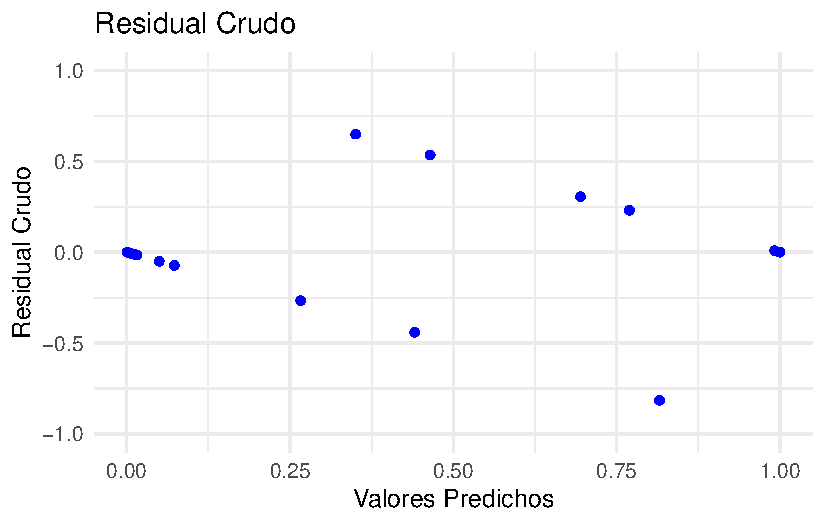
\includegraphics{Modelos_files/figure-pdf/unnamed-chunk-55-1.pdf}\end{minipage}%
%
\begin{minipage}{0.50\linewidth}
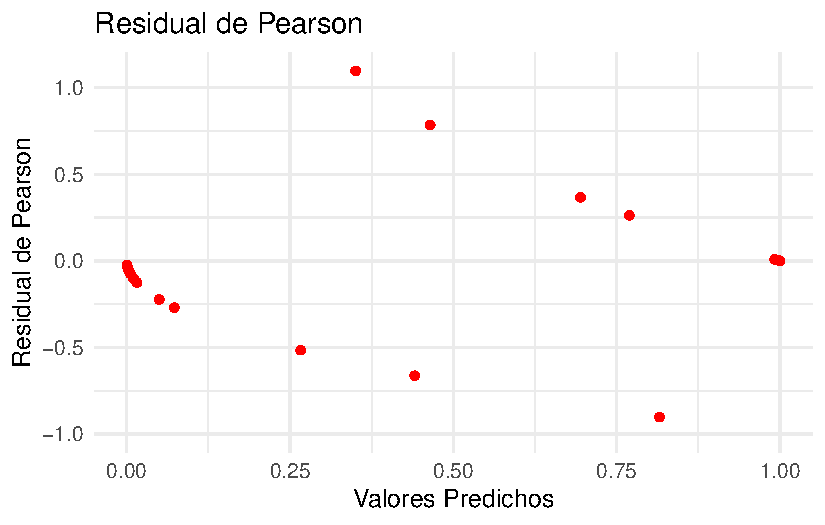
\includegraphics{Modelos_files/figure-pdf/unnamed-chunk-55-2.pdf}\end{minipage}%
\newline
\begin{minipage}{0.50\linewidth}
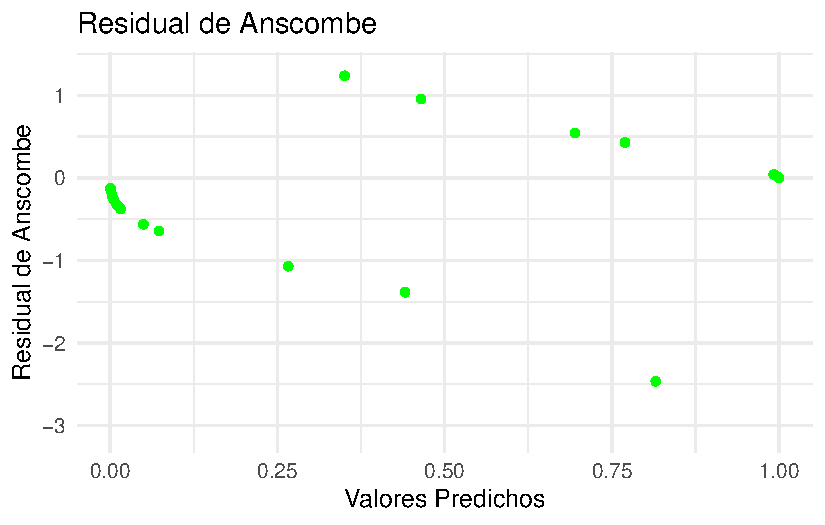
\includegraphics{Modelos_files/figure-pdf/unnamed-chunk-55-3.pdf}\end{minipage}%
%
\begin{minipage}{0.50\linewidth}
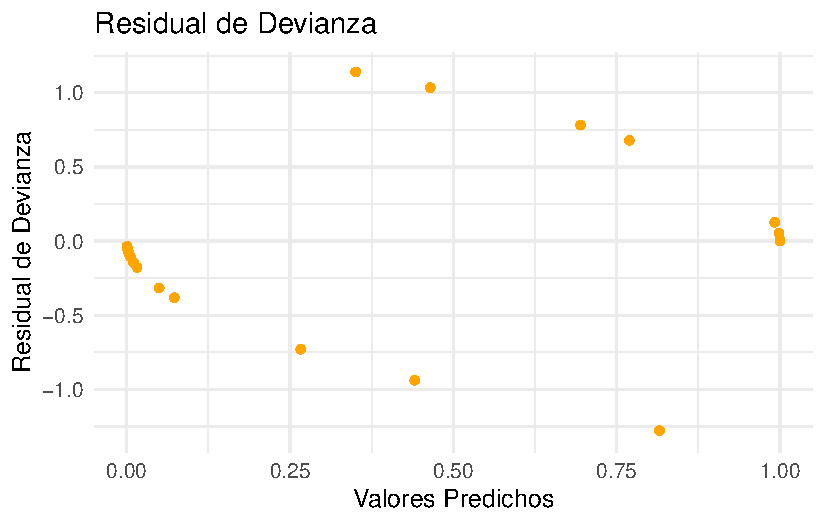
\includegraphics{Modelos_files/figure-pdf/unnamed-chunk-55-4.pdf}\end{minipage}%

\end{figure}%




\end{document}
